\chapter{Order placement evaluation and discussion of results}
\label{chap:analysis}

In the previous Chapter we have built a reinforcement learning environment with the use of the components which were described earlier in Chapter \ref{chap:preliminaries}.
The environment allows to simulate order placement on a historical order book that was described in Chapter \ref{chap:data}.
Furthermore, two agents were introduced: a Q-Learner which learns on private variables; and a Deep Q-Network which learns on market variables.

The aim of this chapter is to make use of this setup and to run simulations and thereby observe whether or not reinforcement learning is indeed capable of optimizing the placement of limit orders.
Therefore, a comprehensive evaluation procedure is being introduced that allows to measure the capabilities of the reinforcement learning agents.
Throughout which use of real world historical order books is being made, as well artificially created order books, whereas the latter allow to define distinctive price trends and eliminate the noise present in real market data.
We first outline the steps of the evaluation procedure.
Subsequently, the real world data sets chosen and their use within the reinforcement learning setup are described.
Finally, we will proceed the evaluation steps in the outlined order.
As a result, this chapter quantifies how effective deep reinforcement learning and the use of the previously constructed market features.

\section{Explanation of the evaluation procedure}
This section explains the procedure undergone in the following sections of this chapter, with which we aim to make a statement about the capabilities of optimizing limit order placement with reinforcement learning and the use of raw market data.
The following points list the steps of the evaluation to be done in chronological order.
\begin{description}
    \item[Empirical investigation: ]
    Section \ref{sec:eval-empirical} investigates the reinforcement learning environment empirically by simulating an agents behaviour that places buy and sell orders for a range of limit levels.
    This will provide knowledge about the limitations of the potential optimization possibilities within the given data set and how well we should expect the reinforcement learners to perform.
    \\
    Results: the \textit{estimated returns} to be received for (1) the optimally chosen limit order or (2) an immediate purchase or sale by using a market order.
    
    \item[Q-Learning agent strategy: ]
    In Section \ref{sec:eval-qlearn}, we make an attempt to build an order placement strategy based on private variables only, by using the Q-Learner.
    This will provide insights of the performance of a naive reinforcement learner and serves as a benchmark for the following simulations proceeded in which we consider market variables.
    \\
    Results: the \textit{average reward} achieved by the Q-Learning agent that uses private variables.

    \item[DQN agent strategy: ]
    Section \ref{sec:eval-dqn} applies market variables to the DQN agent.
    Hereby, we make use of both features, price and size of historical orders (Section \ref{sec:data-feature-1}) as well as the price and size of historical trades (Section \ref{sec:data-feature-2}), separately.
    Similar to the previous evaluation step, we will find the average rewards produced by the agent.
    \\
    Results: the \textit{average reward} achieved by the DQN agent with the use of private variables and (1) historical orders or (2) historical trades.

    \item[DQN agent limitations: ]
    Section \ref{sec:eval-dqn-limitations} aims to determine the capabilities and limitations of the DQN agent in greater detail.
    Therefore, we investigate the chosen actions selected by the agent in order to determine the agents limitations.
    In addition, the agent is applied to an environment which is equipped with an artificially generated order book and will allow to determine to which extent the agent is able to learn from certain price trends.
    \\
    Results: (1) \textit{insights} into when then DQN agent does not perform well and (2) the \textit{average reward} achieved on order books that follow an artificially created trend (upwards, downwards and sine curve).
\end{description}
Given the found results throughout this evaluation, we will be able to determine and quantify to which extent deep reinforcement learning can optimize limit order placement and give reasons for its limitations.

\section{Data sets and their usage in the reinforcement learning setup}
\label{sec:analysis-data-sets}
We have selected two $\sim$30 minute samples of historical order book recordings with which we proceed experiments in this chapter.
Reasons for choosing two very distinguishable data sets include to determine the ability of the learners to react on a variety of market situations.
And, as explained in the following section, the expected return of a learner for buying and selling assets heavily depends on the market price movement and therefore the situations become very different for the data sets in use.
More precisely, \textit{data set I}, as shown in Figure \ref{fig:sample-down-price}), is a downwards trend (indicated by the bid/ask mid-price) and consists of 1132 order book states with a duration of 1681.8 seconds, resulting in 0.67 states per second.
Contrarily, \textit{data set II}, as shown in Figure \ref{fig:sample-up-price}, consists of 1469 order book states with a duration of 1746.0 seconds, resulting in 0.84 states per second, which indicates that there was slightly more pressure in terms of orders placed and cancelled in this data set.
When reinforcement learning is applied, the data sets are split with ratio $2:1$, resulting in a training set of $\sim$20 minutes and a test set of $\sim$10 minutes.
\begin{figure}[H]
    \centering
    \begin{subfigure}[b]{0.45\textwidth}
        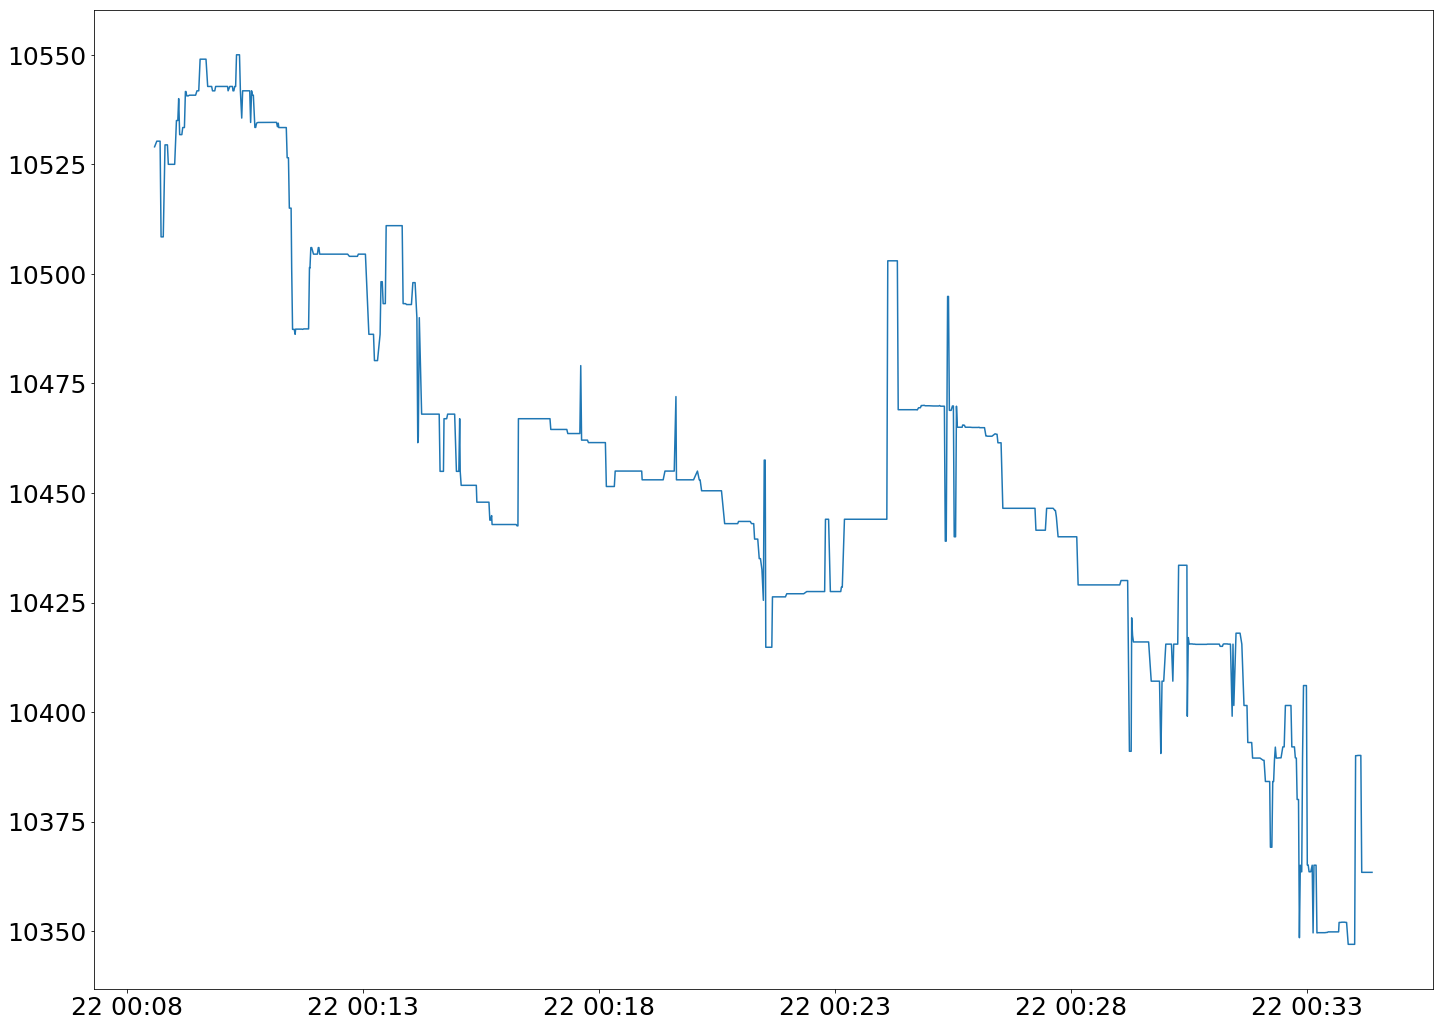
\includegraphics[width=\textwidth]{sample-down-price}
        \caption{30 minute downwards trend}
        \label{fig:sample-down-price}
    \end{subfigure}
    \begin{subfigure}[b]{0.45\textwidth}
        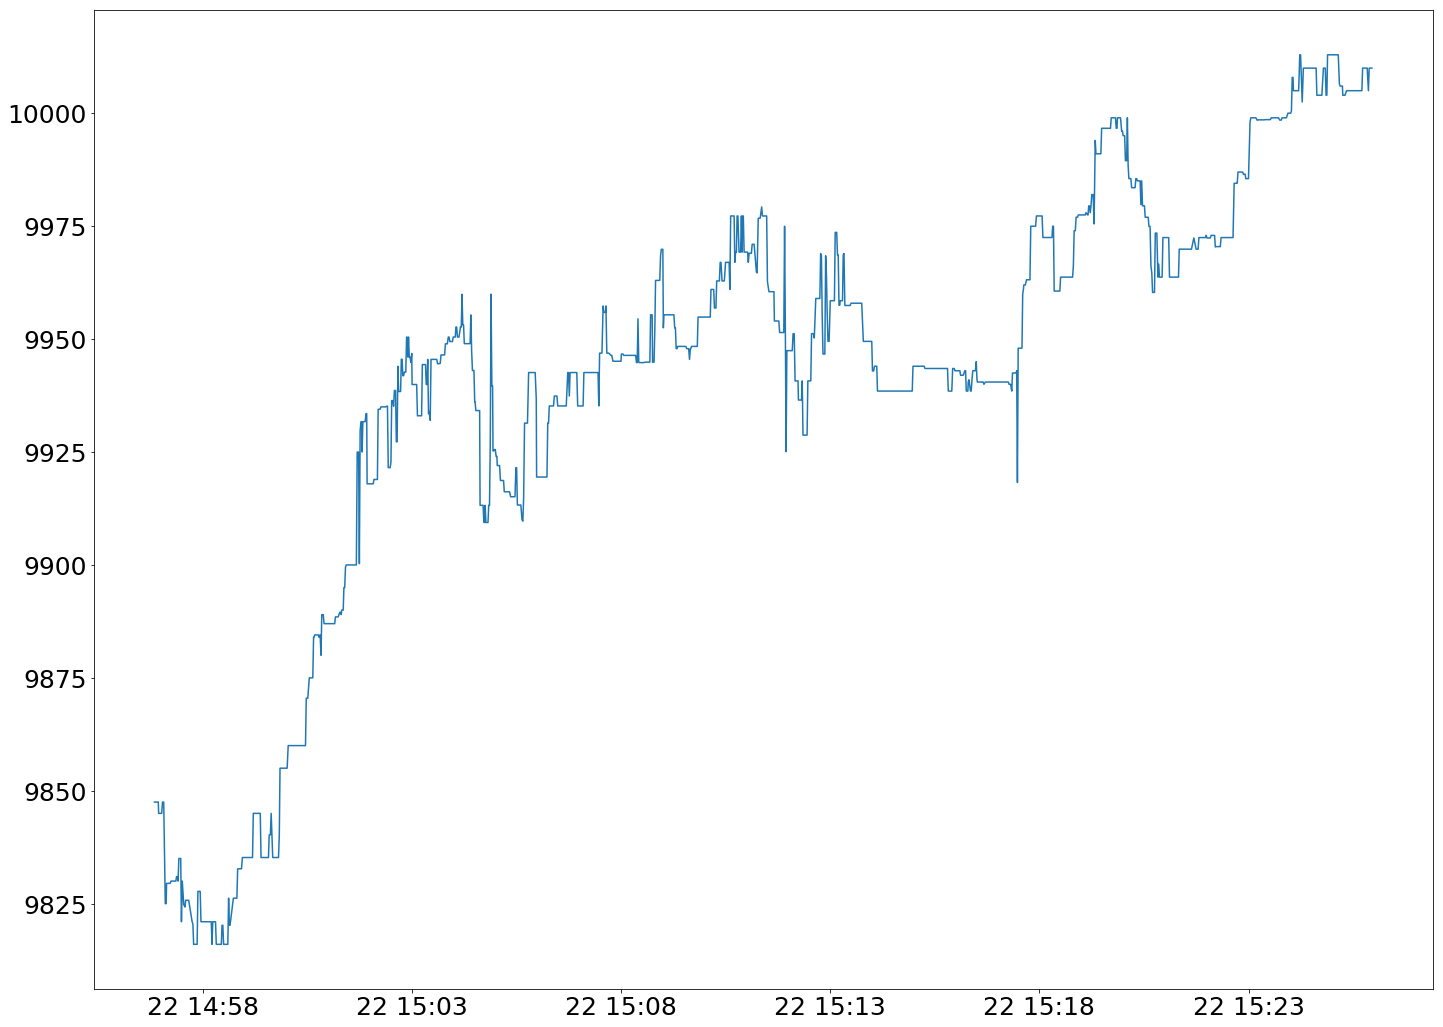
\includegraphics[width=\textwidth]{sample-up-price}
        \caption{30 minute upwards trend}
        \label{fig:sample-up-price}
    \end{subfigure}
    \caption{Bid/ask mid-price of 30 minute order book recordings.}
    \label{fig:sample-price}
\end{figure}

As is explained in Chapter \ref{chap:setup}, the historical data sets are not maintained by the reinforcement learning agents directly but instead by the reinforcement learning environment.
The environment provides an observation state $O$, derived from the data set, to an agent, after which the agent decides to take an action $a$ in form of a limit level.
In turn, the environment prices the order at the received price level and returns the evaluated reward $r$ and the next observation state $O$ to the agent.
This way, the agent can simulate the placement of limit orders, such that, within the given time horizon, the demanded inventory can be either bought or sold.
For each \textit{epoch} an agent proceeds, one order, with a specified inventory and time horizon, is defined and is to be filled.
Therefore, the reinforcement learning environment selects, for each epoch the agent initiates, a range of order book states which form the given time horizon $H$ within which the agent is supposed to complete an order.
\begin{figure}[H]
    \centering
    \makebox[\linewidth]{
        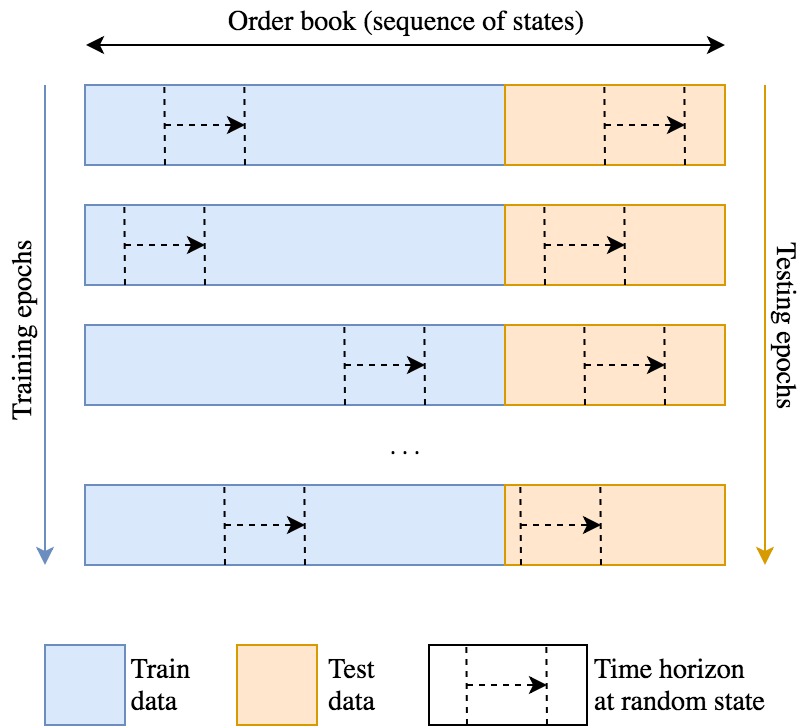
\includegraphics[width=8cm]{images/evaluation-orderbook.png}
    }
    \caption{Order placement training and testing on an order book data set.}
    \label{fig:eval-orderbook-window}
\end{figure}
Figure \ref{fig:eval-orderbook-window} illustrates this process.
A randomly chosen order book state defines the beginning of the time horizon and the set of order book states that fall into this window.
This is very crucial since the states within this time horizon and set of states, not only lead to the observation states received by the agent, but also will determine the outcome of the matching process.
More precisely, for each step the agent takes, a consecutive sequence of order book states (with a total difference of their time stamps of $\Delta{t}$) will be considered by the match engine, as explained in the previous chapter in Section \ref{setup:parameters}.
This process is identical for training and testing, except that the underlying data is different and the agent will not learn from the epochs proceeded during testing and instead will report the achieved rewards.

\section{An empirical investigation of the reinforcement learning environment}
\label{sec:eval-empirical}
This section serves to investigate the relationship between the limit order placement and the received return.
The demonstrated methods are based on the related work described in Section \ref{sec:related-execution-behaviour} and provide the ability to empirically evaluate the reinforcement learning environment (Chapter \ref{chap:setup}).
Therefore we simulate an agent that buys and sells shares at every possible limit level and records the received immediate returns.
The return is denoted by the difference between the market price prior the order placement and the volume weighted average price (VWAP) paid or received respectively, as stated in Eq. \ref{setup:reward}.
As a result, we gain understanding about estimated rewards for limit order placement using the given historical data set.
In addition, these results set a benchmark for the reinforcement learners to come.

The setup of this investigation is as follows.
We investigate the rewards of limit orders placed on progressive increasing time horizons, starting from 10 seconds up to 100 seconds, and therefore demonstrate by hand how a reinforcement learning agent would take discrete time steps.
For each time horizon, we place (e.g. cross-validating) 100 orders of size 1.0 BTC at the beginning of the time horizon whose beginning is defined by a randomly chosen order book state. 
A market order follows for the remainder of shares (if any) once the time horizon is consumed.
The expected return is then formed by the average of the received returns of these 100 orders.
This process is repeated for a range of 201 limit levels ($-100...100$) with step size \$0.10, resulting in orders priced in the range of $p_m-10 \ \dots \ p_m+10$, whereas $p_m$ is the market price before the order was placed.
The limit levels are chosen broadly in order to retrieve understanding about the outcome of a variety of possible actions.
Hence, a total 20'100 orders are submitted for each defined time horizon.
Finally, the investigation is proceeded for both data sets I and II.

\subsection{Order placement behaviour on data set I}
For the data set I, where the market undergoes a downwards trend, the intuition is as follows:
We expect buy orders to result in better returns when placing deep in the order book, meaning with a highly negative limit level.
Since the price tends to fall, the assumption is that an agent is able to buy for a lower price once time has passed.
Therefore, the longer the time horizon, the lower the limit level can be chosen in order to still be able to execute the full amount of shares.
Contrarily, we expect sell orders to provide better returns when the agent crosses the spread with a positive limit level.
The assumption is that in a falling market it is unlikely that market participants are willing to buy for higher prices and therefore the agent must place sell orders higher in the book in order to sell immediately.
Otherwise, the longer the time horizon, the less return an agent would retrieve as the market order after the order has not been filled becomes costly.
This investigation is shown in Figure \ref{fig:behvaiour-down} for time horizons of 10, 30, 60 and 100 seconds respectively.
The x-axis indicates the placement of the order at limit levels reaching from -100 to +100 and the y-axis indicates the average received return.

With a time horizon of only 10 seconds left, the expected behaviour is, however, proven wrong.
For buy orders, shown in Figure \ref{fig:behvaiour-down-10s-buy}, the returns suggest to place the orders close to the spread, but still on the opposing side, at a limit level of $\sim$+5.
The spike at limit level $\sim$-5 indicates that the overall best return was provided at this level, however it comes with the risk that the orders fails to execute, indicated by the downwards spike also close to level $\sim$-5.
For selling within 10 seconds, as shown in Figure \ref{fig:behvaiour-up-10s-sell}, the best return is given when crossing the spread with a positive limit level of $\sim$+50.

With an increased time horizon of a total of 30 seconds, as shown in Figures \ref{fig:behvaiour-down-30s-buy} and \ref{fig:behvaiour-down-30s-sell}, the expected behaviour becomes more apparent.
Positive returns can be achieved by posting buy orders deep in the order book.
Therefore, we can expect that in the given market situation an agent would be able to execute the order partially at very low limit levels and for the unexecuted part a market order would follow.
The most dense range of positive returns seen around the limit levels just below the spread.
Orders placed deeper in the book result oftentimes in slightly lower returns, which indicates that the orders were only filled partially and expensive market orders followed.
Crossing the spread causes increasingly lower returns, the more positive the limit level is chosen, as a result of agents willingness to immediately buy at an increasing price.
The opposite effect occurs while selling assets.
Market orders higher in the book result in result in better returns than limit orders deep in the book.
Interestingly, orders which were placed very deep in the book, at limit level $\sim$-50 and below, are rewarded better than the ones close to the spread.
This is most likely a consequence of a minority of orders which were partially filled at this level during the cross-validation process.

With time horizons of 60 and 100 seconds the expected behaviour of the orders is clearly apparent.
Buy orders, as shown in Figures \ref{fig:behvaiour-down-60s-buy} and \ref{fig:behvaiour-down-100s-buy}, achieve most return when placed very deep in the order book.
However, when placed too deep, at level -100, the return is slightly less as a result of unexecuted orders which had to be completed with market orders.
In addition, positive limit levels become stable since there are more sellers in the market with the extended time horizon and therefore very high placed orders have the same effect as limit orders posted only slightly above the spread.
Furthermore, placing orders very deep in the book have the same effect as when placing the order just below the spread, that is, there are no traders willing to buy at such a high price and therefore market orders follow once the time has passed.
\vfill
\newpage
\begin{figure}[H]
    \centering
    \begin{subfigure}[b]{0.45\textwidth}
        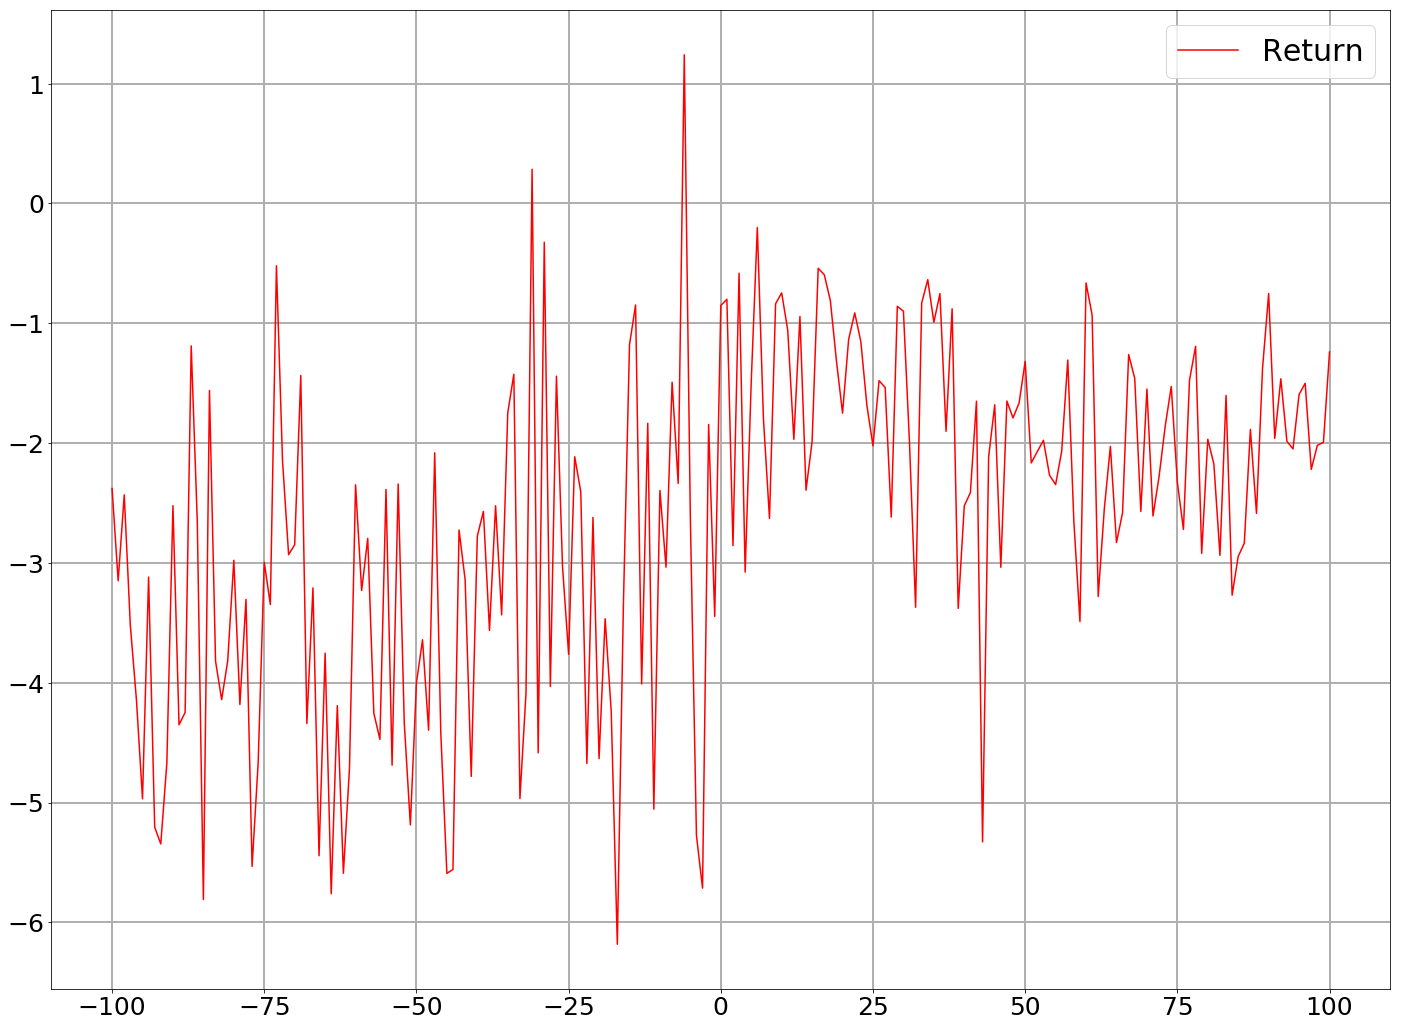
\includegraphics[width=\textwidth]{images/behaviour-10s-buy.png}
        \caption{Returns of buy orders within 10 seconds}
        \label{fig:behvaiour-down-10s-buy}
    \end{subfigure}
    \begin{subfigure}[b]{0.45\textwidth}
        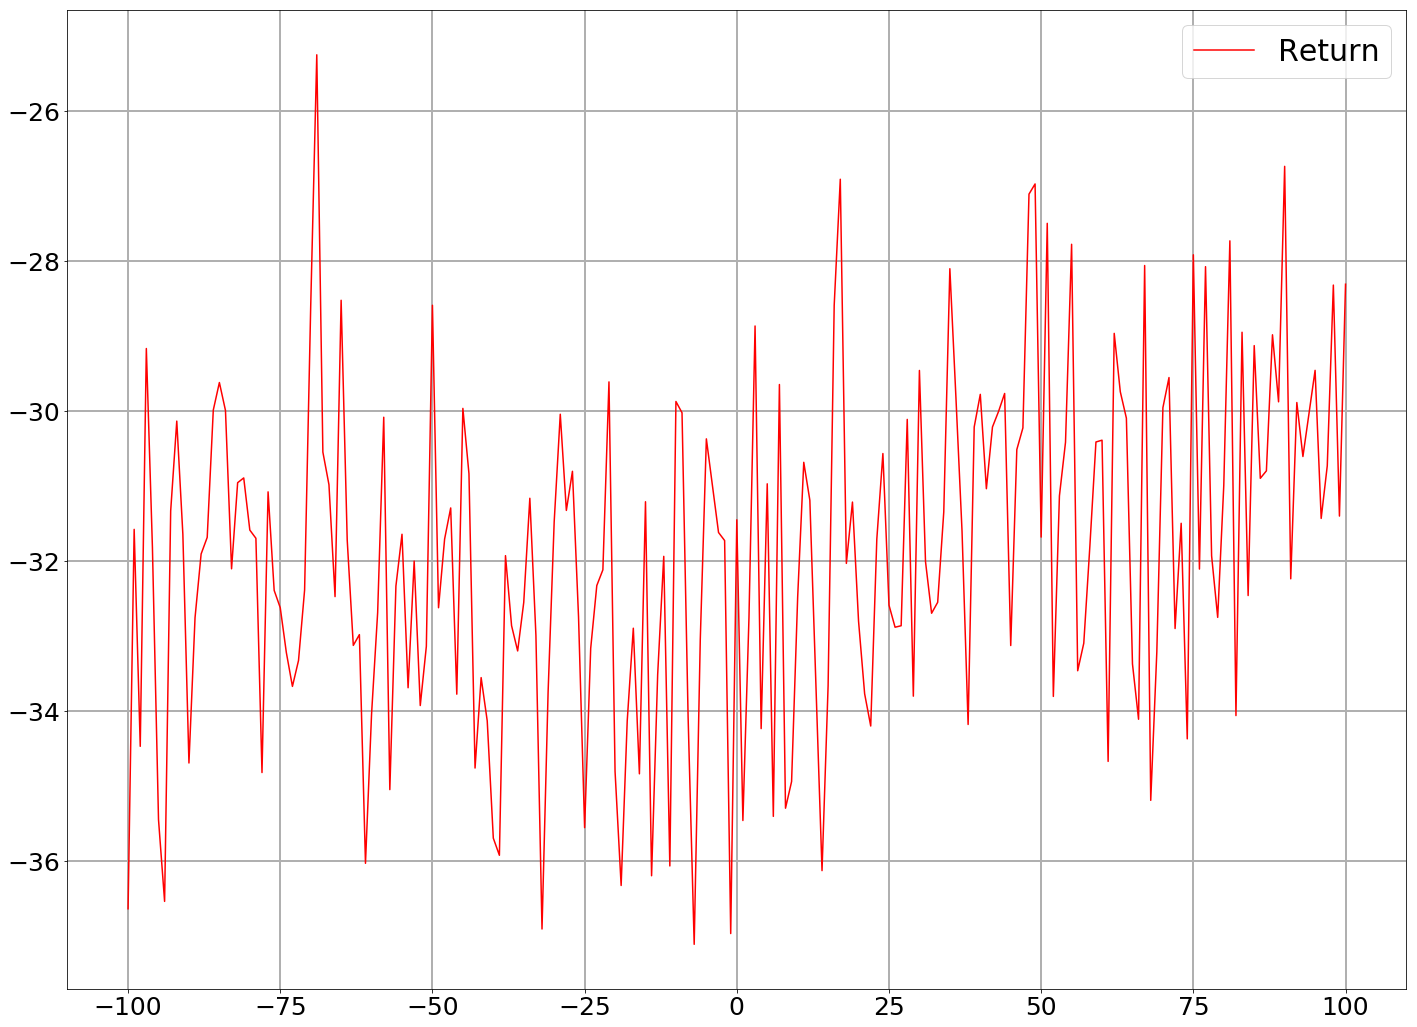
\includegraphics[width=\textwidth]{images/behaviour-10s-sell.png}
        \caption{Returns of sell orders within 10 seconds}
        \label{fig:behvaiour-down-10s-sell}
    \end{subfigure}
    \begin{subfigure}[b]{0.45\textwidth}
        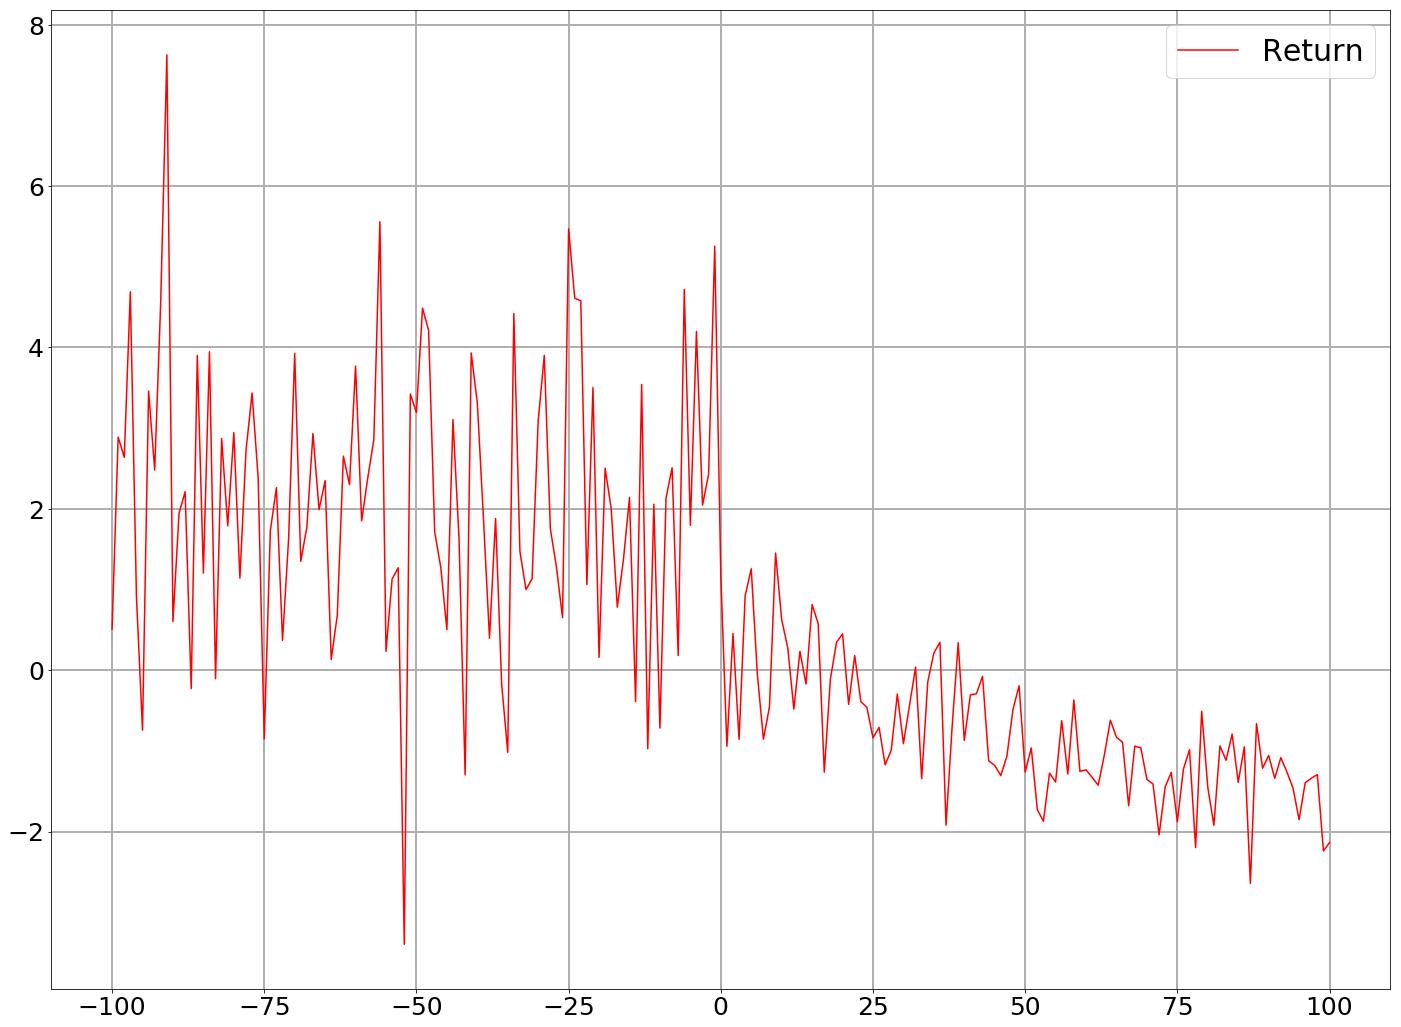
\includegraphics[width=\textwidth]{images/behaviour-30s-buy.png}
        \caption{Returns of buy orders within 30 seconds}
        \label{fig:behvaiour-down-30s-buy}
    \end{subfigure}
    \begin{subfigure}[b]{0.45\textwidth}
        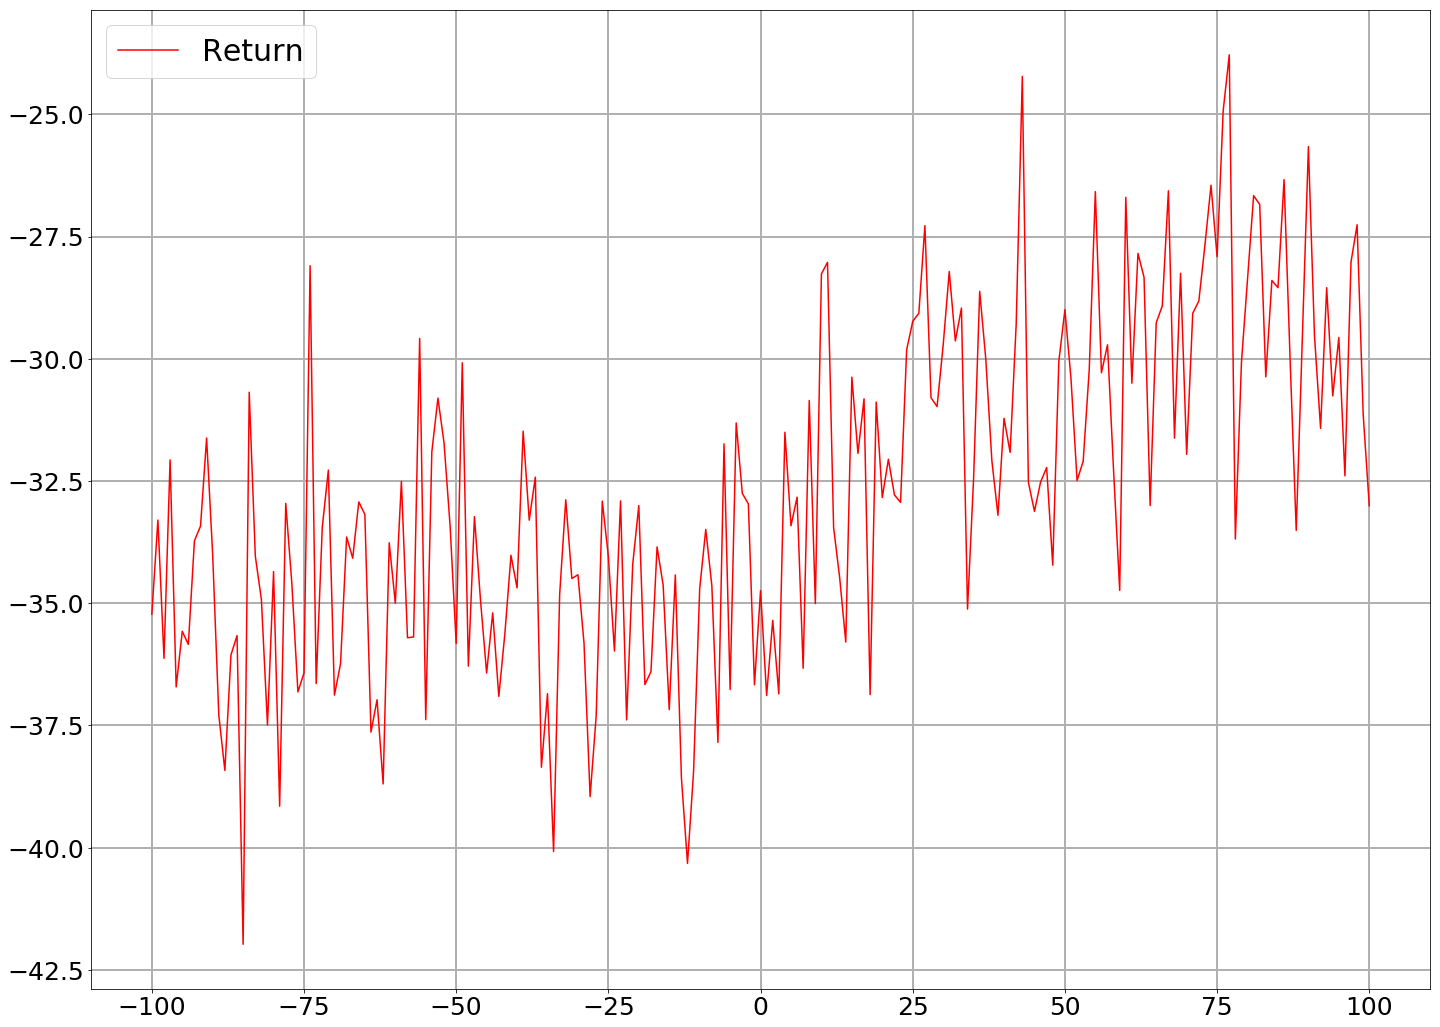
\includegraphics[width=\textwidth]{images/behaviour-30s-sell.png}
        \caption{Returns of sell orders within 30 seconds}
        \label{fig:behvaiour-down-30s-sell}
    \end{subfigure}
    \begin{subfigure}[b]{0.45\textwidth}
        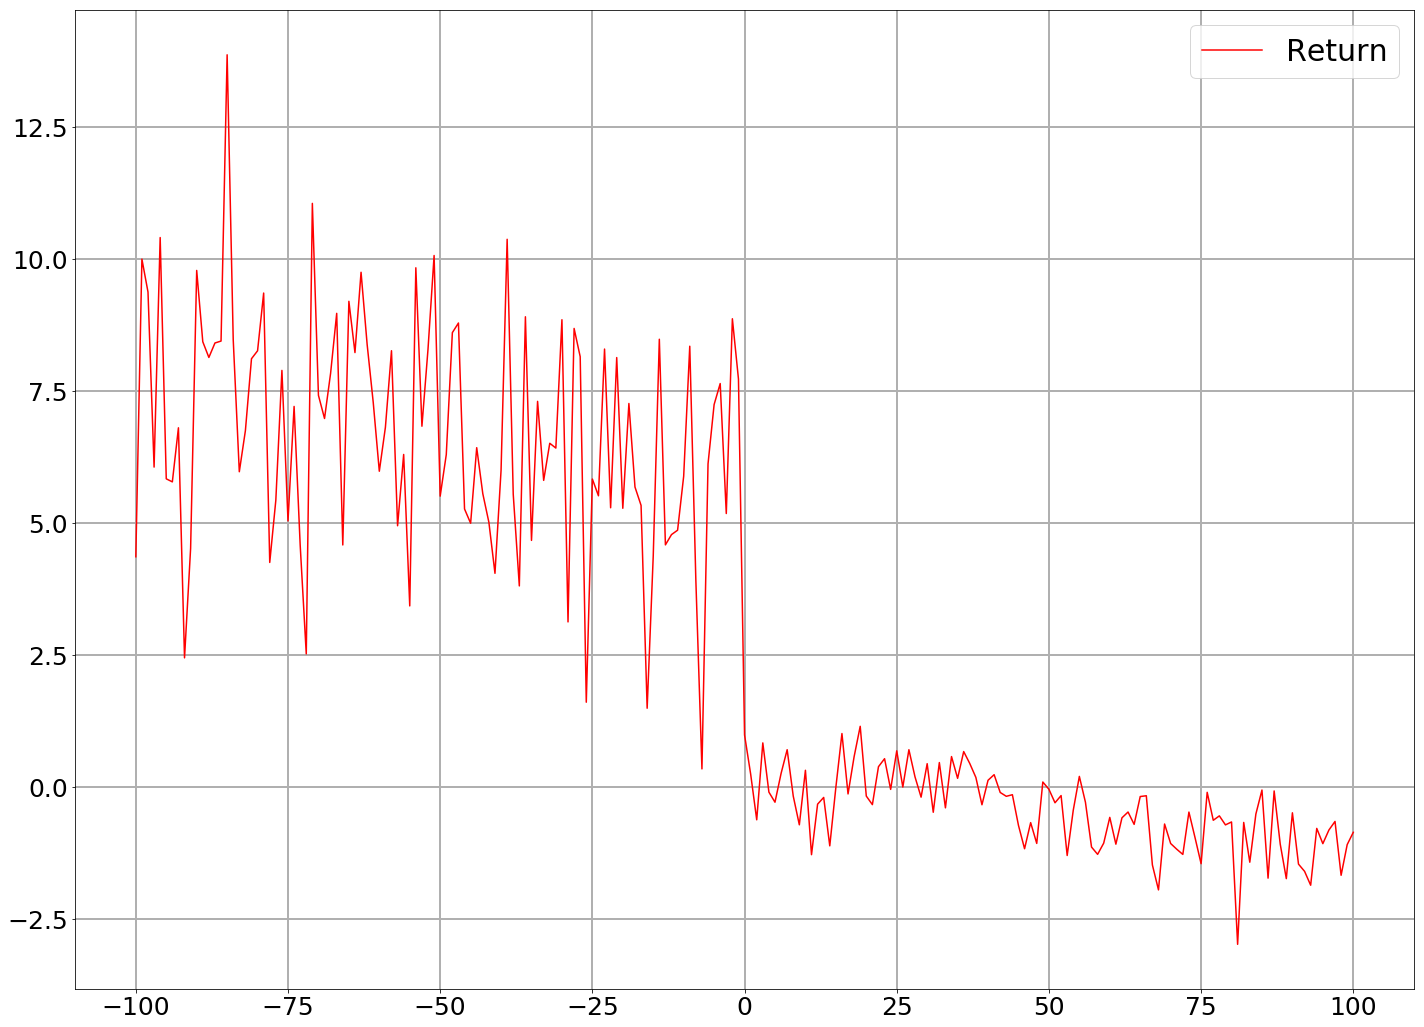
\includegraphics[width=\textwidth]{images/behaviour-60s-buy.png}
        \caption{Returns of buy orders within 60 seconds}
        \label{fig:behvaiour-down-60s-buy}
    \end{subfigure}
    \begin{subfigure}[b]{0.45\textwidth}
        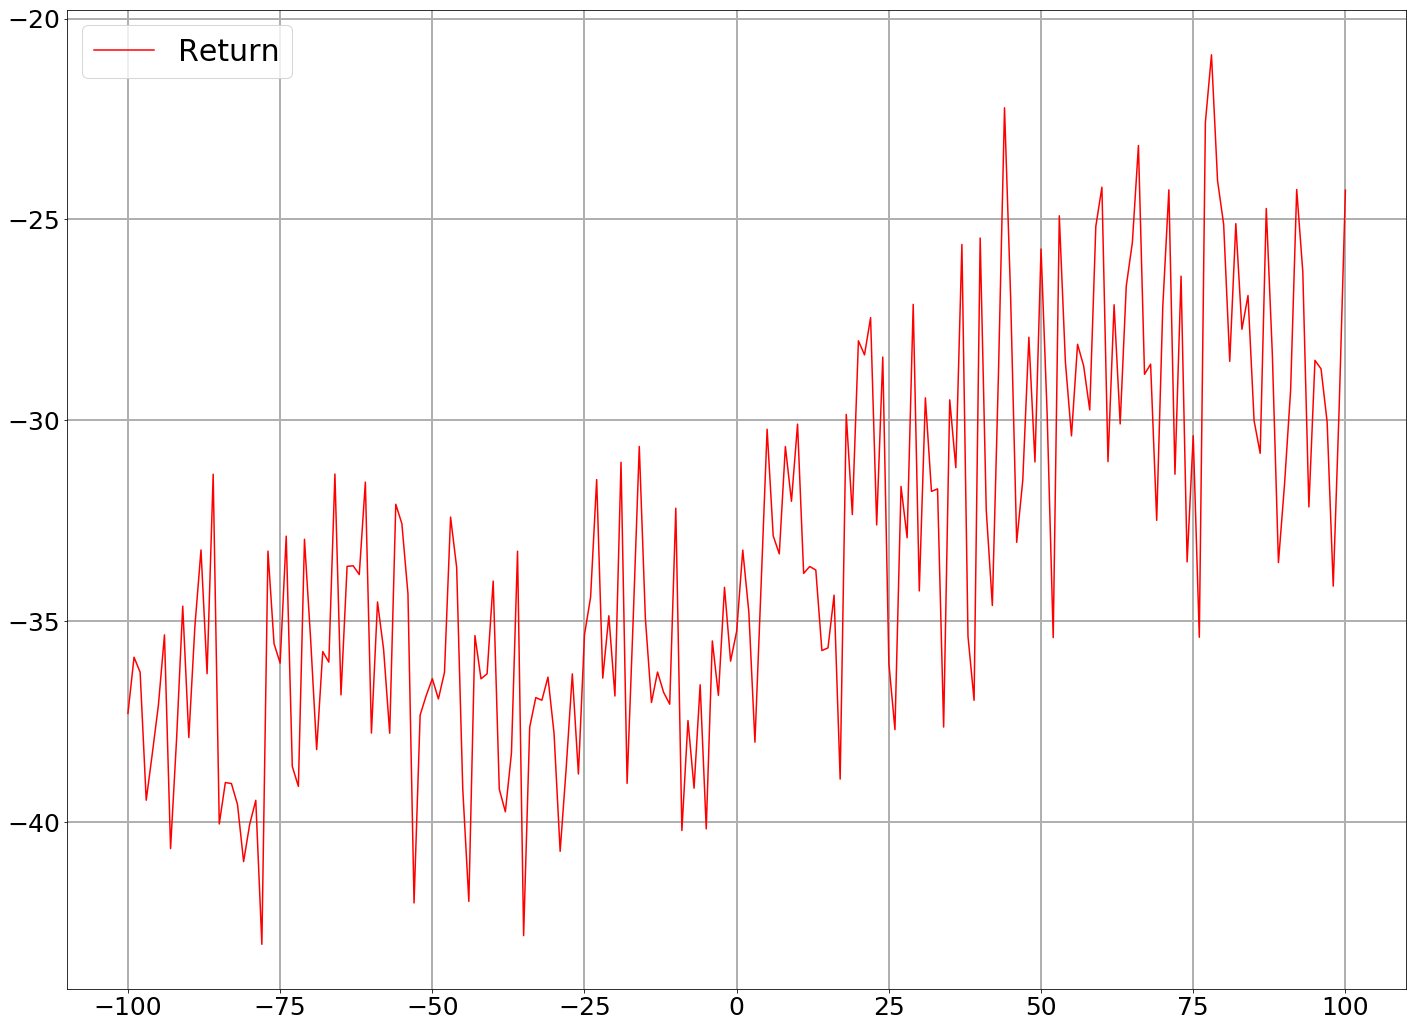
\includegraphics[width=\textwidth]{images/behaviour-60s-sell.png}
        \caption{Returns of sell orders 60 seconds}
        \label{fig:behvaiour-down-60s-sell}
    \end{subfigure}
    \begin{subfigure}[b]{0.45\textwidth}
        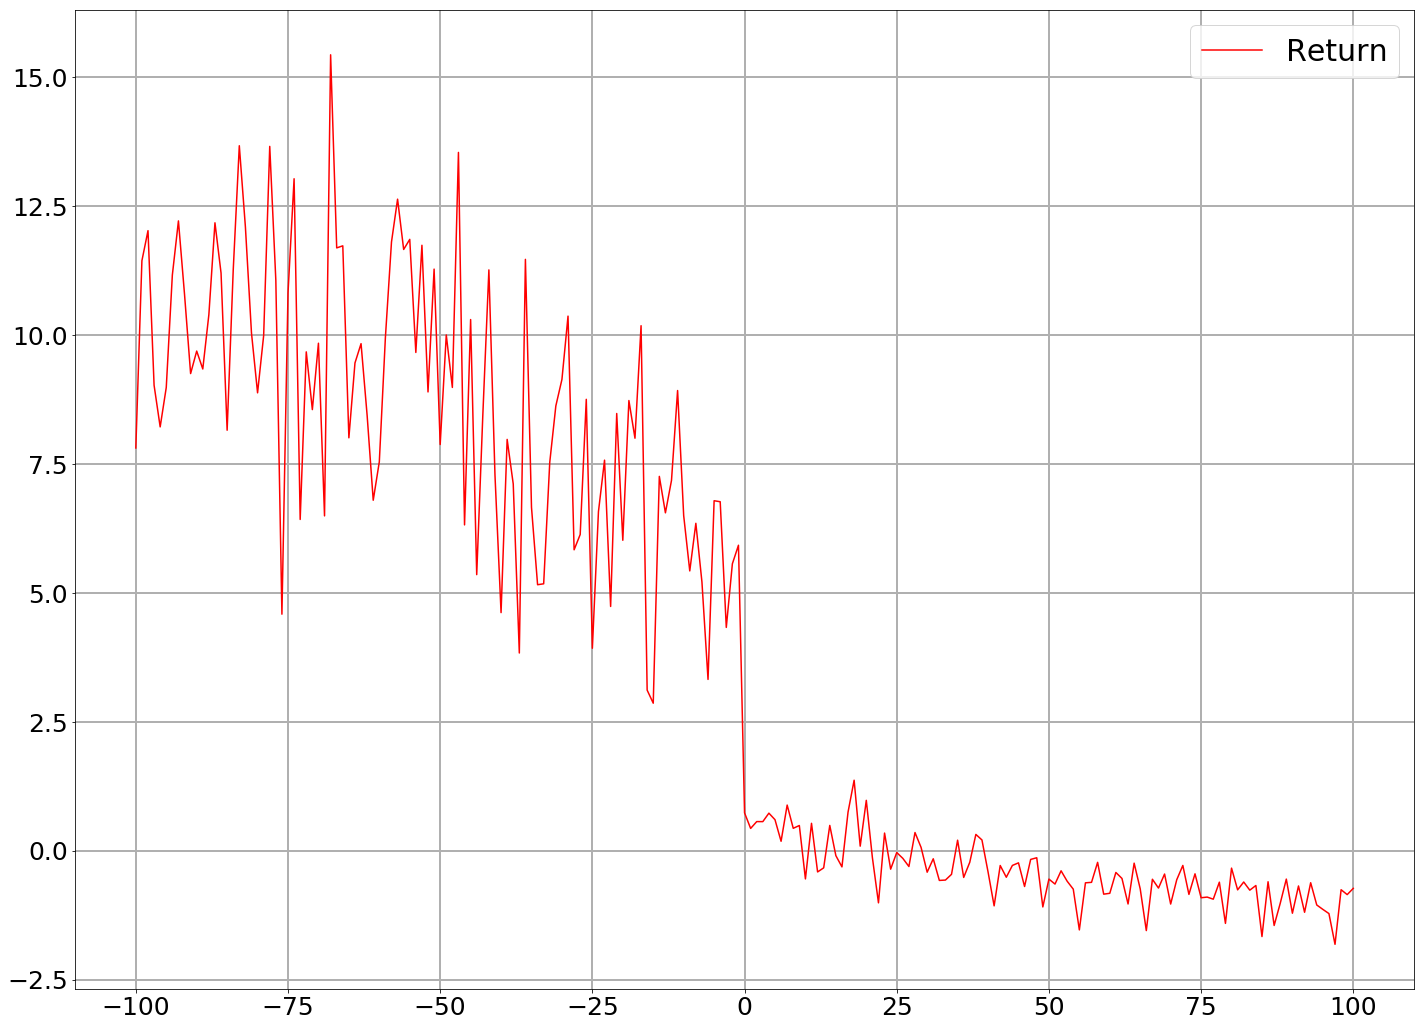
\includegraphics[width=\textwidth]{images/behaviour-100s-buy.png}
        \caption{Returns of buy orders 100 seconds}
        \label{fig:behvaiour-down-100s-buy}
    \end{subfigure}
    \begin{subfigure}[b]{0.45\textwidth}
        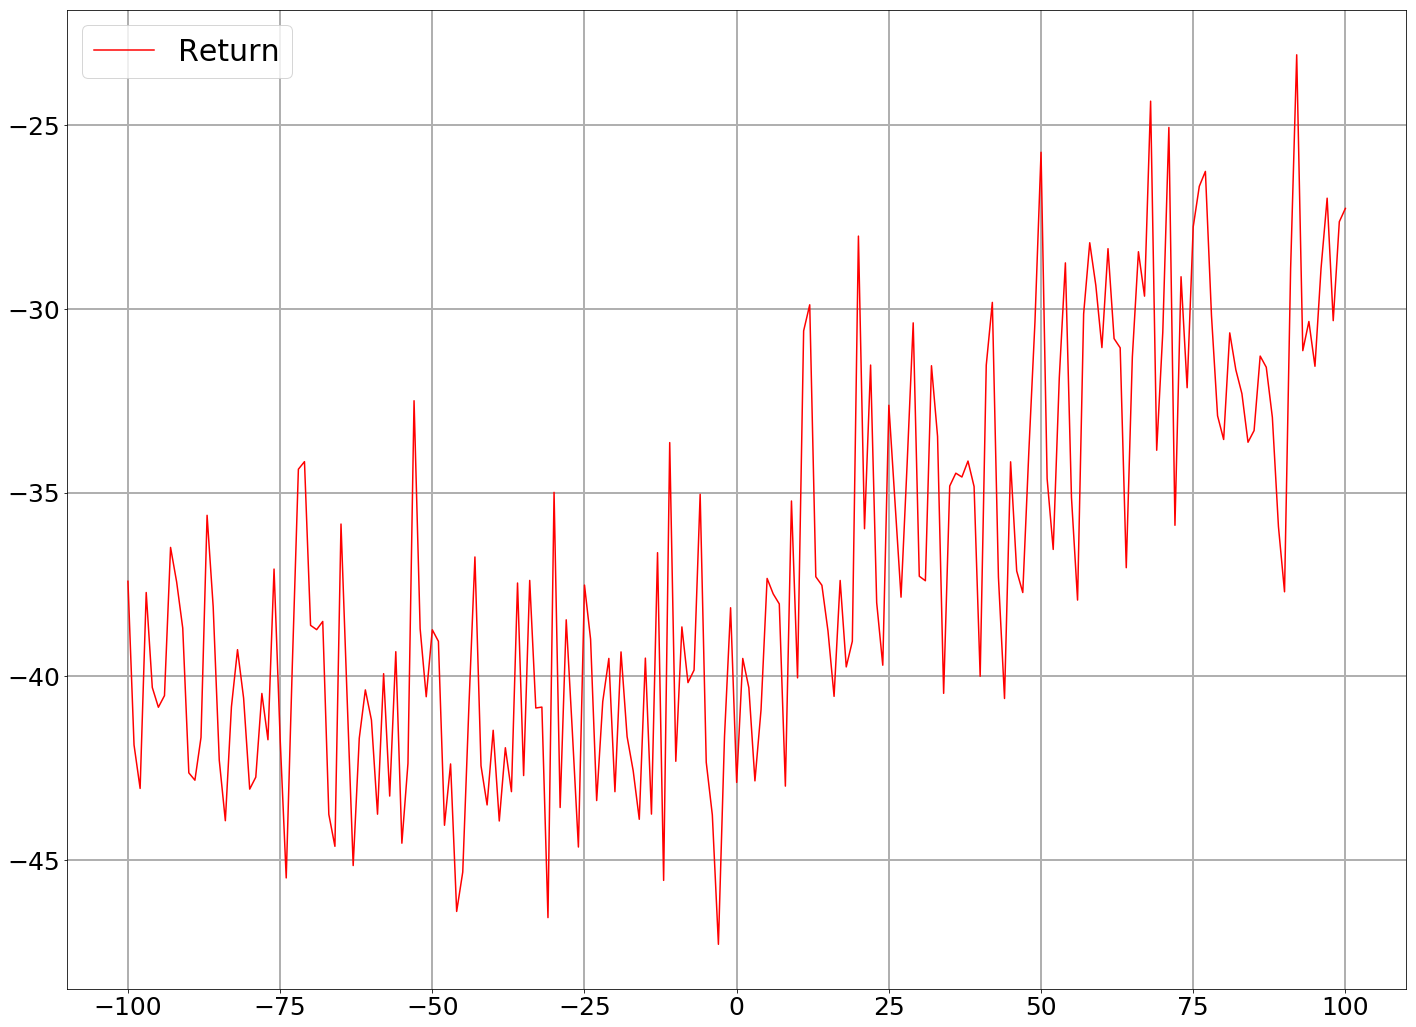
\includegraphics[width=\textwidth]{images/behaviour-100s-sell.png}
        \caption{Returns of sell orders 100 seconds}
        \label{fig:behvaiour-down-100s-sell}
    \end{subfigure}
    \caption{Returns of buy and sell orders executed within 10, 30, 60 and 100 seconds on data set I.}
    \label{fig:behvaiour-down}
\end{figure}

\begin{figure}[H]
    \centering
    \begin{subfigure}[b]{0.45\textwidth}
        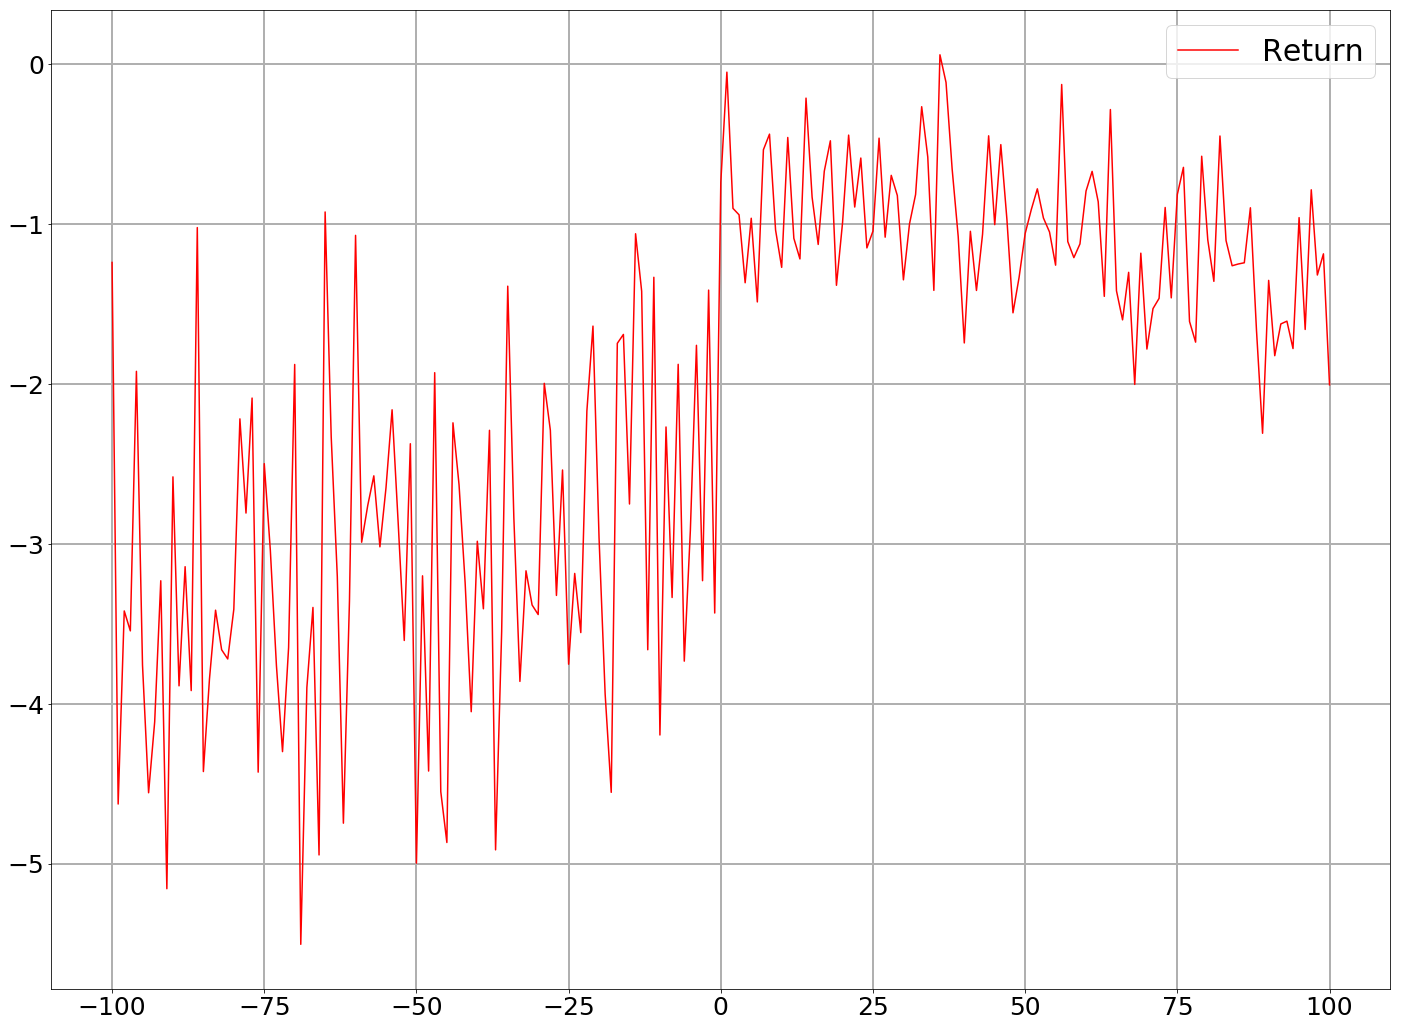
\includegraphics[width=\textwidth]{images/behaviour-up-10s-buy.png}
        \caption{Returns of buy orders within 10 seconds}
        \label{fig:behvaiour-up-10s-buy}
    \end{subfigure}
    \begin{subfigure}[b]{0.45\textwidth}
        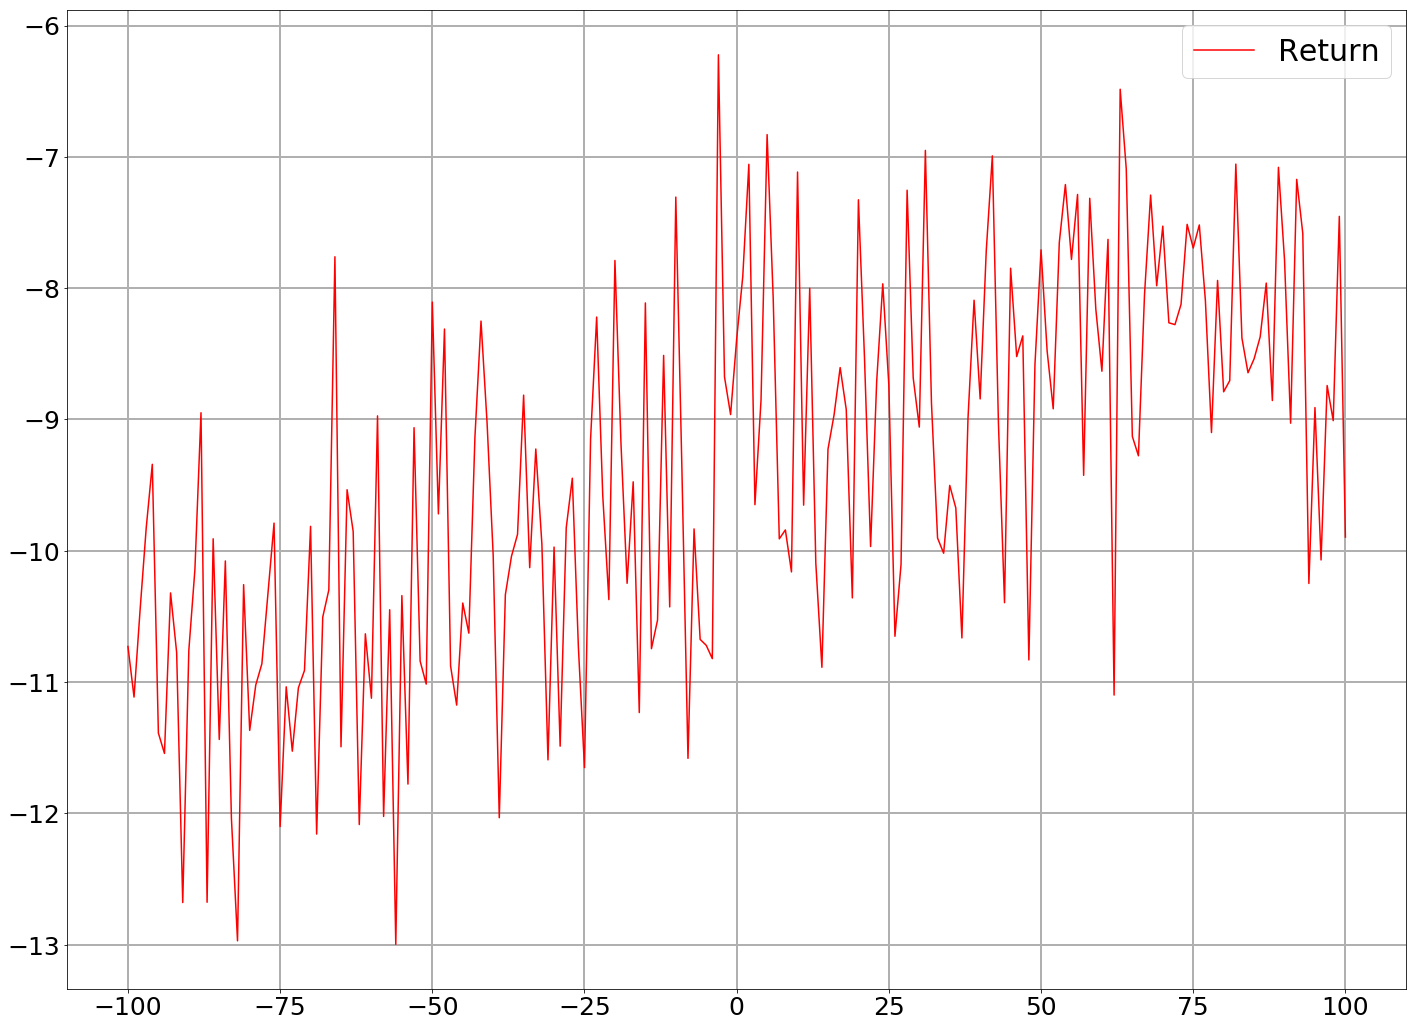
\includegraphics[width=\textwidth]{images/behaviour-up-10s-sell.png}
        \caption{Returns of sell orders within 10 seconds}
        \label{fig:behvaiour-up-10s-sell}
    \end{subfigure}
    \begin{subfigure}[b]{0.45\textwidth}
        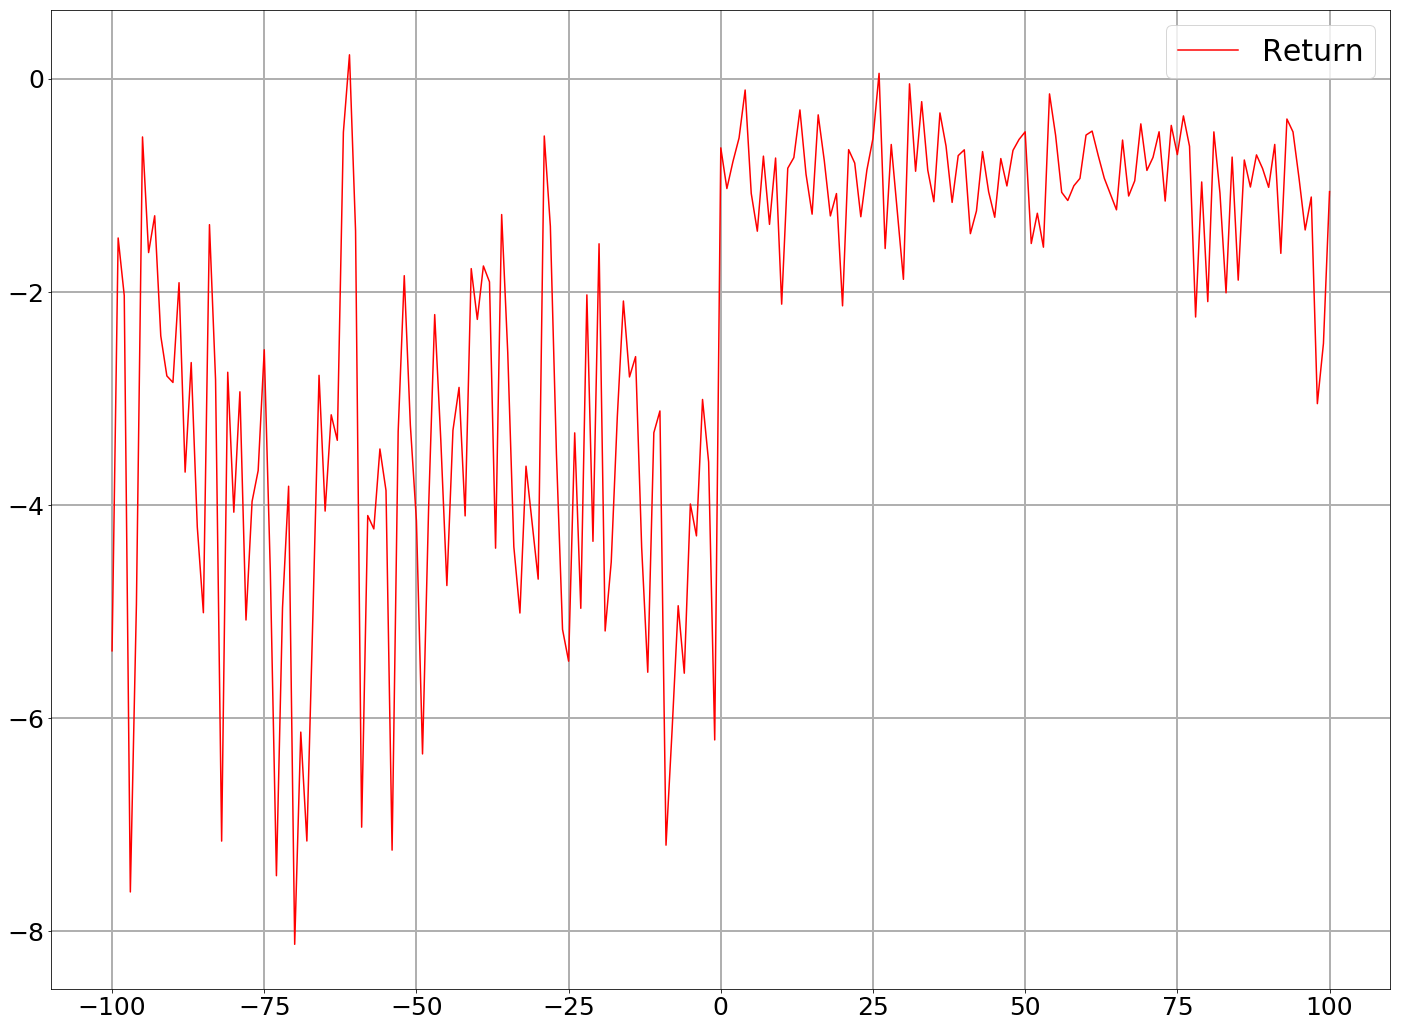
\includegraphics[width=\textwidth]{images/behaviour-up-30s-buy.png}
        \caption{Returns of buy orders within 30 seconds}
        \label{fig:behvaiour-up-30s-buy}
    \end{subfigure}
    \begin{subfigure}[b]{0.45\textwidth}
        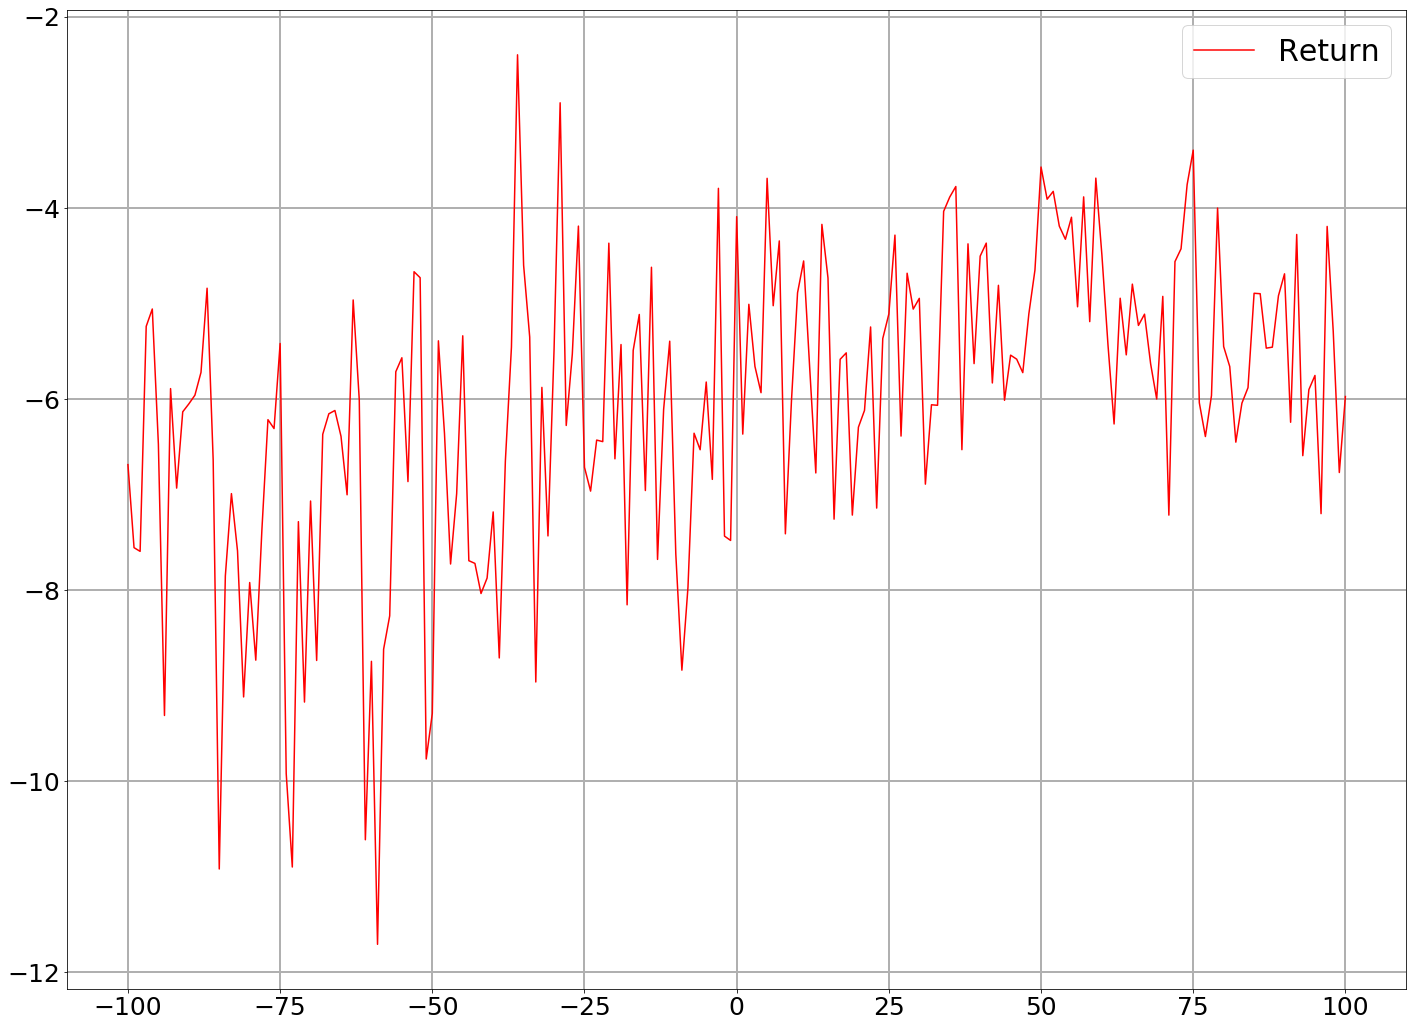
\includegraphics[width=\textwidth]{images/behaviour-up-30s-sell.png}
        \caption{Returns of sell orders within 30 seconds}
        \label{fig:behvaiour-up-30s-sell}
    \end{subfigure}
    \begin{subfigure}[b]{0.45\textwidth}
        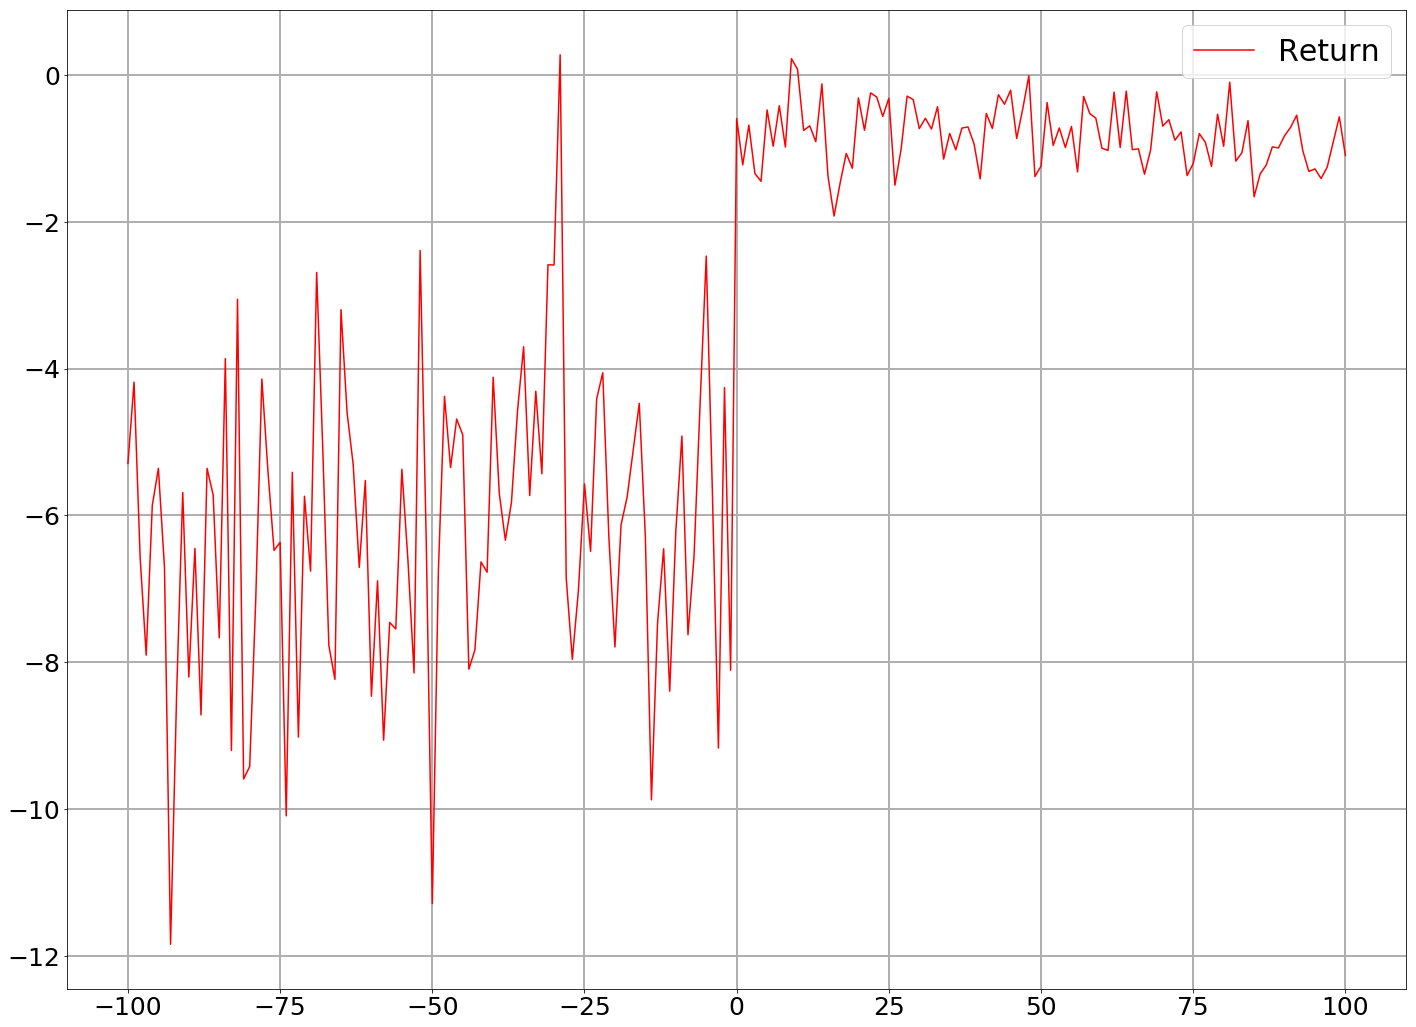
\includegraphics[width=\textwidth]{images/behaviour-up-60s-buy.png}
        \caption{Returns of buy orders within 60 seconds}
        \label{fig:behvaiour-up-60s-buy}
    \end{subfigure}
    \begin{subfigure}[b]{0.45\textwidth}
        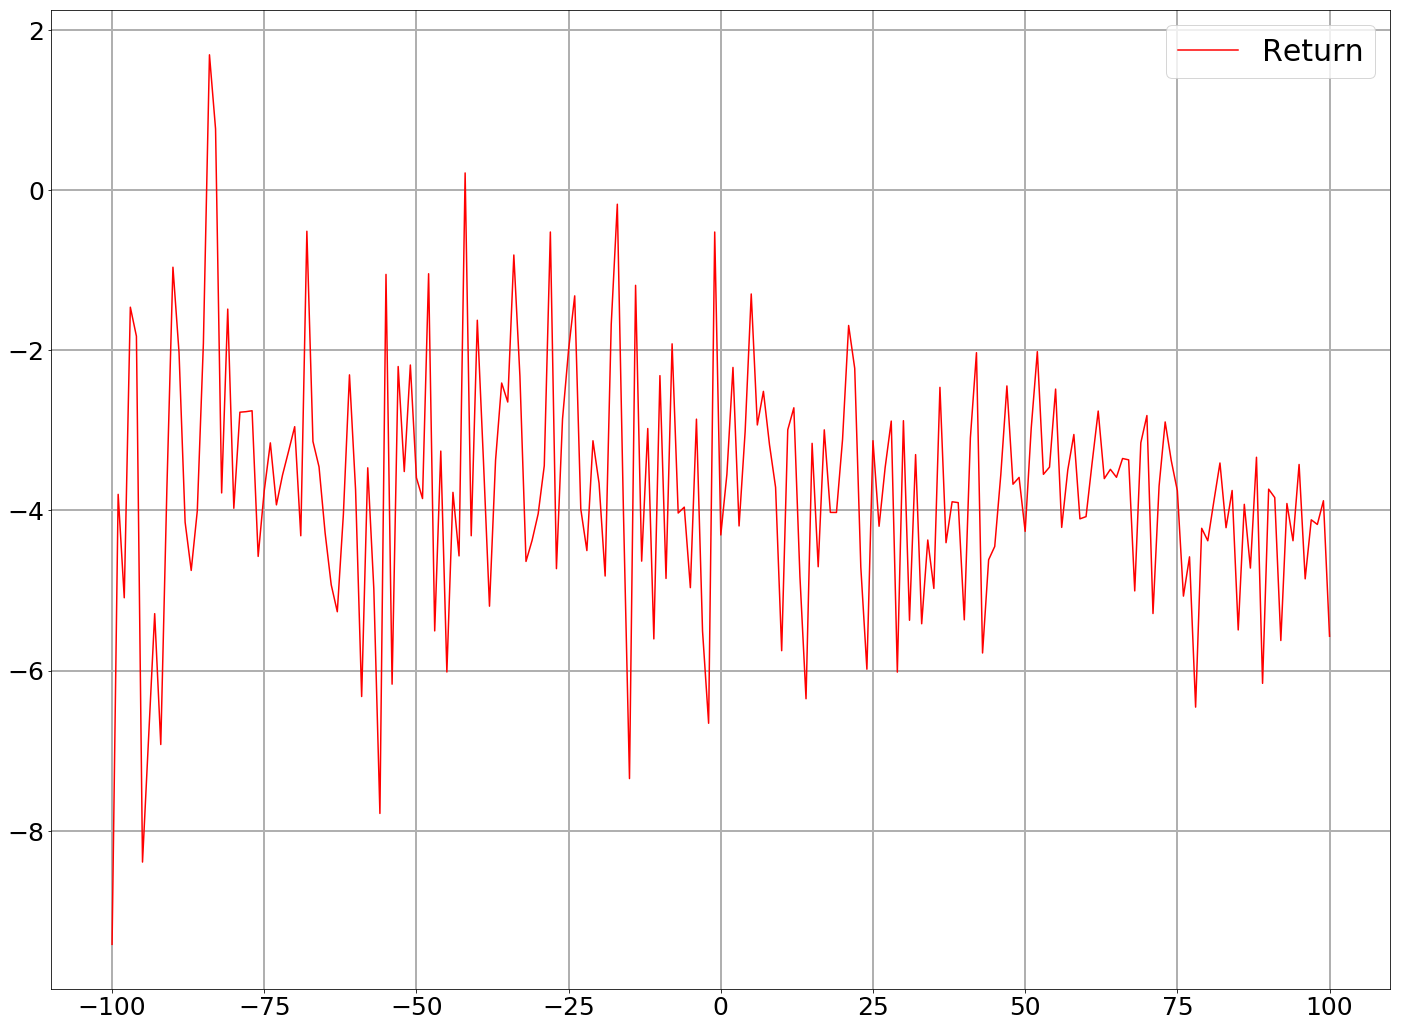
\includegraphics[width=\textwidth]{images/behaviour-up-60s-sell.png}
        \caption{Returns of sell orders 60 seconds}
        \label{fig:behvaiour-up-60s-sell}
    \end{subfigure}
    \begin{subfigure}[b]{0.45\textwidth}
        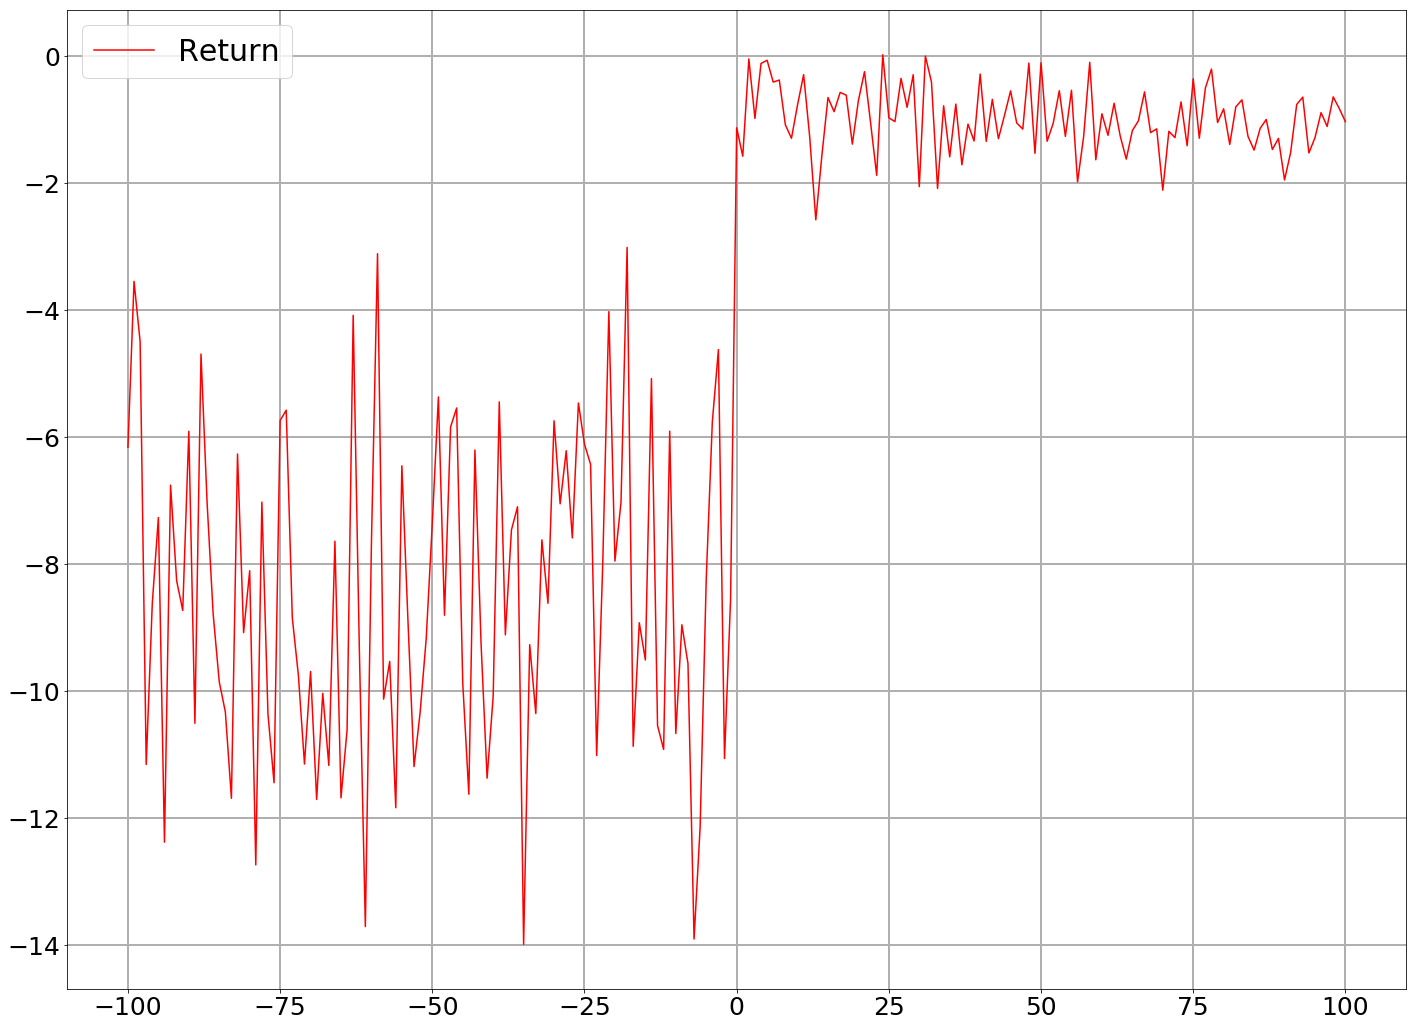
\includegraphics[width=\textwidth]{images/behaviour-up-100s-buy.png}
        \caption{Returns of buy orders 100 seconds}
        \label{fig:behvaiour-up-100s-buy}
    \end{subfigure}
    \begin{subfigure}[b]{0.45\textwidth}
        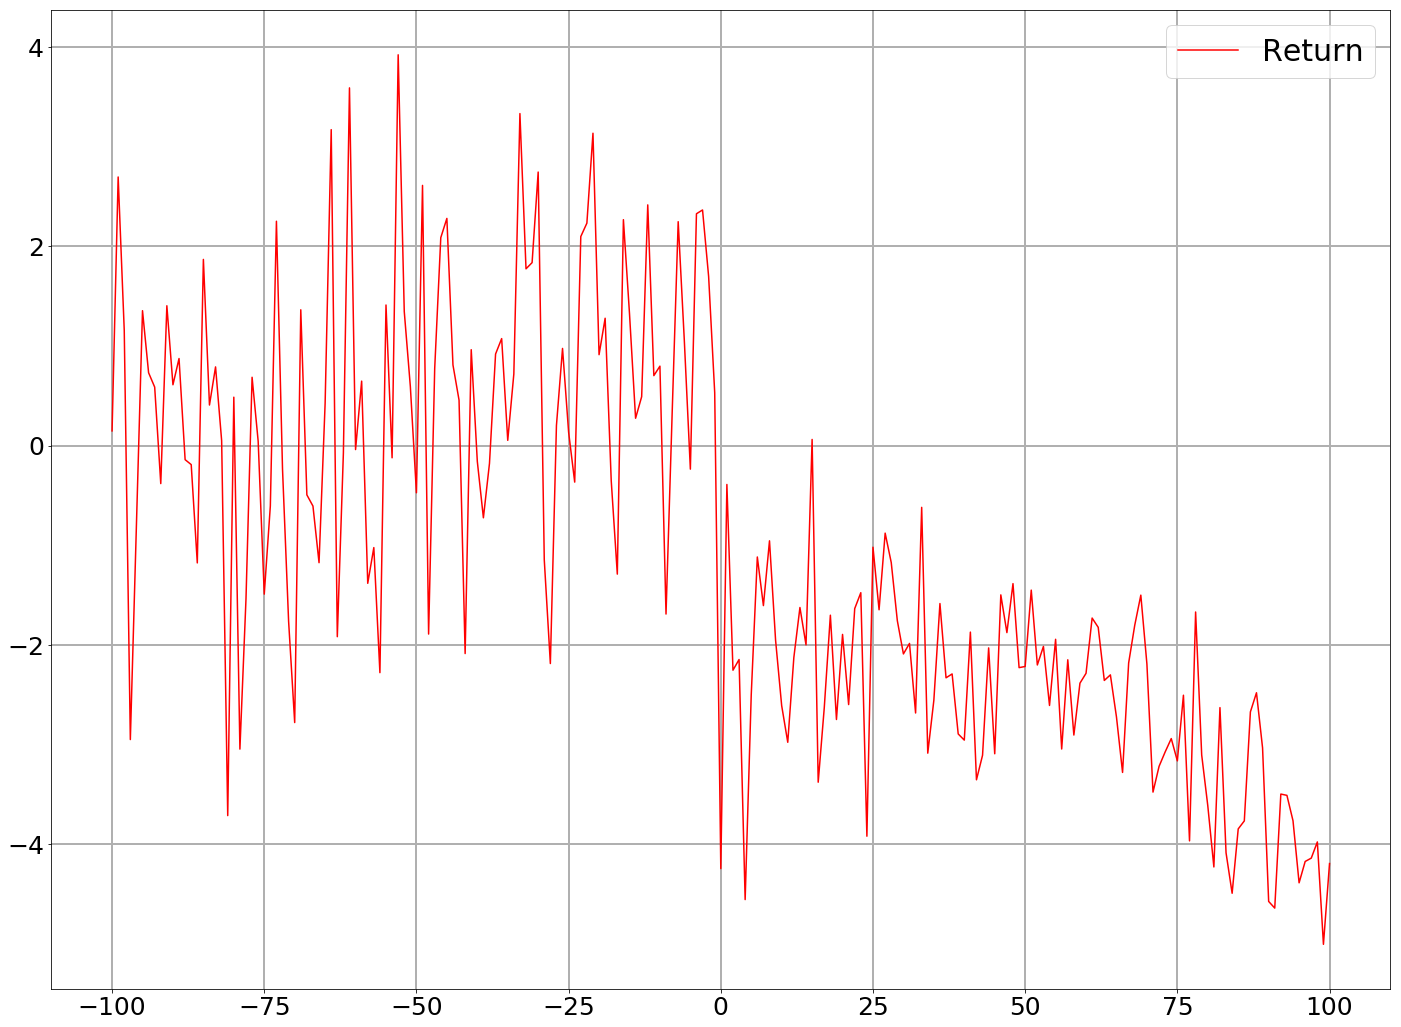
\includegraphics[width=\textwidth]{images/behaviour-up-100s-sell.png}
        \caption{Returns of sell orders 100 seconds}
        \label{fig:behvaiour-up-100s-sell}
    \end{subfigure}
    \caption{Returns of buy and sell orders executed within 10, 30, 60 and 100 seconds on data set II.}
    \label{fig:behvaiour-up}
\end{figure}

\subsection{Order placement behaviour on data set II}
For the data set II, which shows an upwards price trend, the intuition is the opposite as for the investigation using data set I.
We expect buy orders to result in better returns when immediately filled, that is, when the agent crosses the spread and places the order high in the book.
The assumption is that, as time passes and the market price rises, other traders become less willing to sell for the market price or lower.
Therefore, the longer the time horizon given to the agent, the more critical it becomes to execute immediately, as otherwise shares would have to be bought to an increased market price.
Contrarily, better returns with sell orders are expected when placed deep in the book, meaning to be sold at a higher price.
The assumption is that as the price rises, market participants become more likely to buy assets for higher prices.
Hence, the longer the time horizon, the deeper the agent should place a limit sell order in the book, as this will likely not require a following market order due to (partially) unexecuted shares.
We investigate these assumptions by proceeding the same experiment as in the previous section, as shown in Figure \ref{fig:behvaiour-up}, with time horizons of 10, 30, 60 and 100 seconds respectively.
The x-axis denotes the placement of the order at limit levels reaching from -100 to +100 and the y-axis indicates the average received return.

The returns of buy orders filled within a time horizon of 10 seconds, as shown in Figure \ref{fig:behvaiour-up-10s-buy}, correlate with the above stated assumptions.
The highest returns are achieved when crossing the spread and although limit levels in the range of 1-50 tend to perform the same, and considering the risk of paying a premium, the wisest choice for the agent would be to choose the level closest to the spread.
The sell orders placed, with a time horizon of 10 seconds, contradict the assumptions, as shown in Figure \ref{fig:behvaiour-up-10s-sell}.
The agent is rewarded the most when choosing a price for the order at market price, as indicated by the limit level 0, that is on the spread.
A highly negative limit level causes to receive approximately \$3.00 less than when placing at the suggested market price.

With 30 seconds left to buy 1.0 BTC, in Figure \ref{fig:behvaiour-up-30s-buy}, the orders placed above the spread become stable for any such limit level, much more so than with the same time horizon in the previous investigation with the data set I.
This is likely due to the higher order pressure of the data set II, as described in Section \ref{sec:analysis-data-sets}, as there are more market participants willing to sell.
The return curve that indicates sell orders placed by an agent, shown in Figure \ref{fig:behvaiour-up-30s-sell}, becomes more evenly distributed.
Therefore, limit orders tend to become more rewarding and an agent might benefit from a slight increase in price within the given time horizon.

This pattern becomes clearly appararent when a time horizon of 60 and 100 seconds was given, as shown in Figures \ref{fig:behvaiour-up-60s-sell} and \ref{fig:behvaiour-up-100s-sell} respectively.
With the increased time horizon, the assumptions stated in the beginning of this section are confirmed and the agent, when trying to sell shares, should indeed place orders deep in the order book.
As time passes and the market price rises, market participants are willing to buy for an increasing price and an agent is expected to be able to sell all assets for such an increased price without the need of a following market order.
Contrarily, if the agent decides to offer to sell the assets for a decreasing price, as indicated by the higher limit levels above the spread, the less reward would can be expected.
More precisely, for a time horizon of 100 seconds, the agent is expected to receive up to \$7.00 less when choosing to cross the spread with a limit level of +100, compared to some negative limit level.
Figures \ref{fig:behvaiour-up-60s-buy} and \ref{fig:behvaiour-up-100s-buy} which show the expected results of an agent that buys assets within the 60 and 100 seconds respectively.
As is evident, during this uprising market, the expected damage can be minimized by crossing the spread and buying immediately.
The advice stated before remains: the agent should choose a price a few steps (\$0.10) above the market price as there is enough liquidity in the market to buy the demanded number of assets.

\subsection{Conclusion of empirical analysis}
The results of the empirical analysis proceeded on data set I and II have shown that the tendency of limit order execution is as follows:
during a downwards trend of the market price, buying assets can be optimized by placing limit orders deep in the order book and the least loss is taken when selling assets immediately to the market price.
Contrarily, during an upwards market price trend, buying assets is suggested using a market order and selling can be optimized by placing the sell orders deep in the order book.
This effect becomes more apparent when a longer time horizon is given for an order, as for shorter time horizons the order placement process gets either intercepted by short term fluctuations or a lack of market participants providing volume to buy and sell assets.
In this analysis, the orders placed had to be completely filled without the ability to make intermediary steps of cancellations and replacements of the order within the given time horizon.
It is therefore to be evaluated by the reinforcement learners whether or not such adaptions to the order will result in a more favorable reward.
In order to have a measure of comparison for the reinforcement learning agents to come, Table \ref{tbl:analysis-empirical-summary} summarizes the findings and shows the expected rewards for (1) the optimal limit level chosen and (2) an immediate completion of the order using a market order.
\begin{table}[H]
\centering
\begin{tabular}{l|l|l|}
\cline{2-3}
& \textbf{Limit order (optimal)} & \textbf{\begin{tabular}[c]{@{}l@{}}Market order\end{tabular}} \\ \hline
\multicolumn{1}{|l|}{\textbf{Buy (I)}}   & 15.20          & -0.05                                                           \\ \hline
\multicolumn{1}{|l|}{\textbf{Sell (I)}}  & -27.70         & -27.70                                                          \\ \hline
\multicolumn{1}{|l|}{\textbf{Buy (II)}}  & -1.06          & -1.06                                                           \\ \hline
\multicolumn{1}{|l|}{\textbf{Sell (II)}} & 3.68          & -1.72                                                           \\ \hline
\end{tabular}
\caption{Summary of rewards derived form the empirical analysis.}
\label{tbl:analysis-empirical-summary}
\end{table}

\section{Q-Learning without market variables}
\label{sec:eval-qlearn}
The previous section provided knowledge about the possibilities of the agent when placing buy and sell orders using the reinforcement learning environment and with the underlying data set I and II.
The expected behaviour for each limit level has been observed under two significantly different market situations.
For each such observation, a fixed time horizon was chosen for which an order was residing in the order book, followed by a market order in case the order has not been filled completely.
It has been shown that during an upwards trend, market participants are willing to buy and sell shares for higher prices and contrarily, during a downwards trend for lower prices.
However, it has been observed that an agent would therefore indeed be able to, if limit orders were placed accordingly, minimize the price to pay, respectively maximize the price for which to receive, the assets.

This section aims to investigate whether or not a Q-Learning agent, as described in Chapter \ref{chap:setup} (Section \ref{setup:q-learning}), can reproduce the optimal achieved results shown in the previous section.
Therefore the agent is allowed to cancel its order after every 10 seconds and place a new order with the remaining inventory, until the time horizon is fully consumed.
For both data sets (I and II) an independent learning experiment is being proceeded, whereas the agent is supposed to either buy or sell shares.
For each such experiment, the training is limited to 5000 epochs and 1000 orders are being back-tested on the test set.
The Q-Learning agent is set up as follows:
the learning rate $\alpha=0.1$ is chosen small due to extensive amounts of steps the agent will make throughout the epochs.
The discount factor $\gamma=0.7$ is chosen slightly in favour of immediate rewards in the hope to prevent the agent from running out of time which would result in a following market order.
Initially, the exploration constant $\epsilon$ is set to 0.1 but then multiplied by an epsilon decay factor for each step taken by the agent, such that $\epsilon=\sim0.8$ once training is completed.
This allows the agent first to explore the action space and then exploit on the learned optimal actions to take.

As a result of this setup, four observations were made and for each of which the training and testing results are stated below.
During training, the mean rewards given and average action chosen for each epoch are recorded.
Using the training model, a backtest is run on the test data sets, whereas the agent executes orders and chooses the learned optimal action to take.
The result of which is shown as the average reward received while doing so.
The difference to the occurring costs of a market order then serves as the guideline of how well the algorithm performs.

\subsection{Results of training and testing on data set I and II}

\begin{figure}
    \centering
    \begin{subfigure}[b]{0.4\textwidth}
        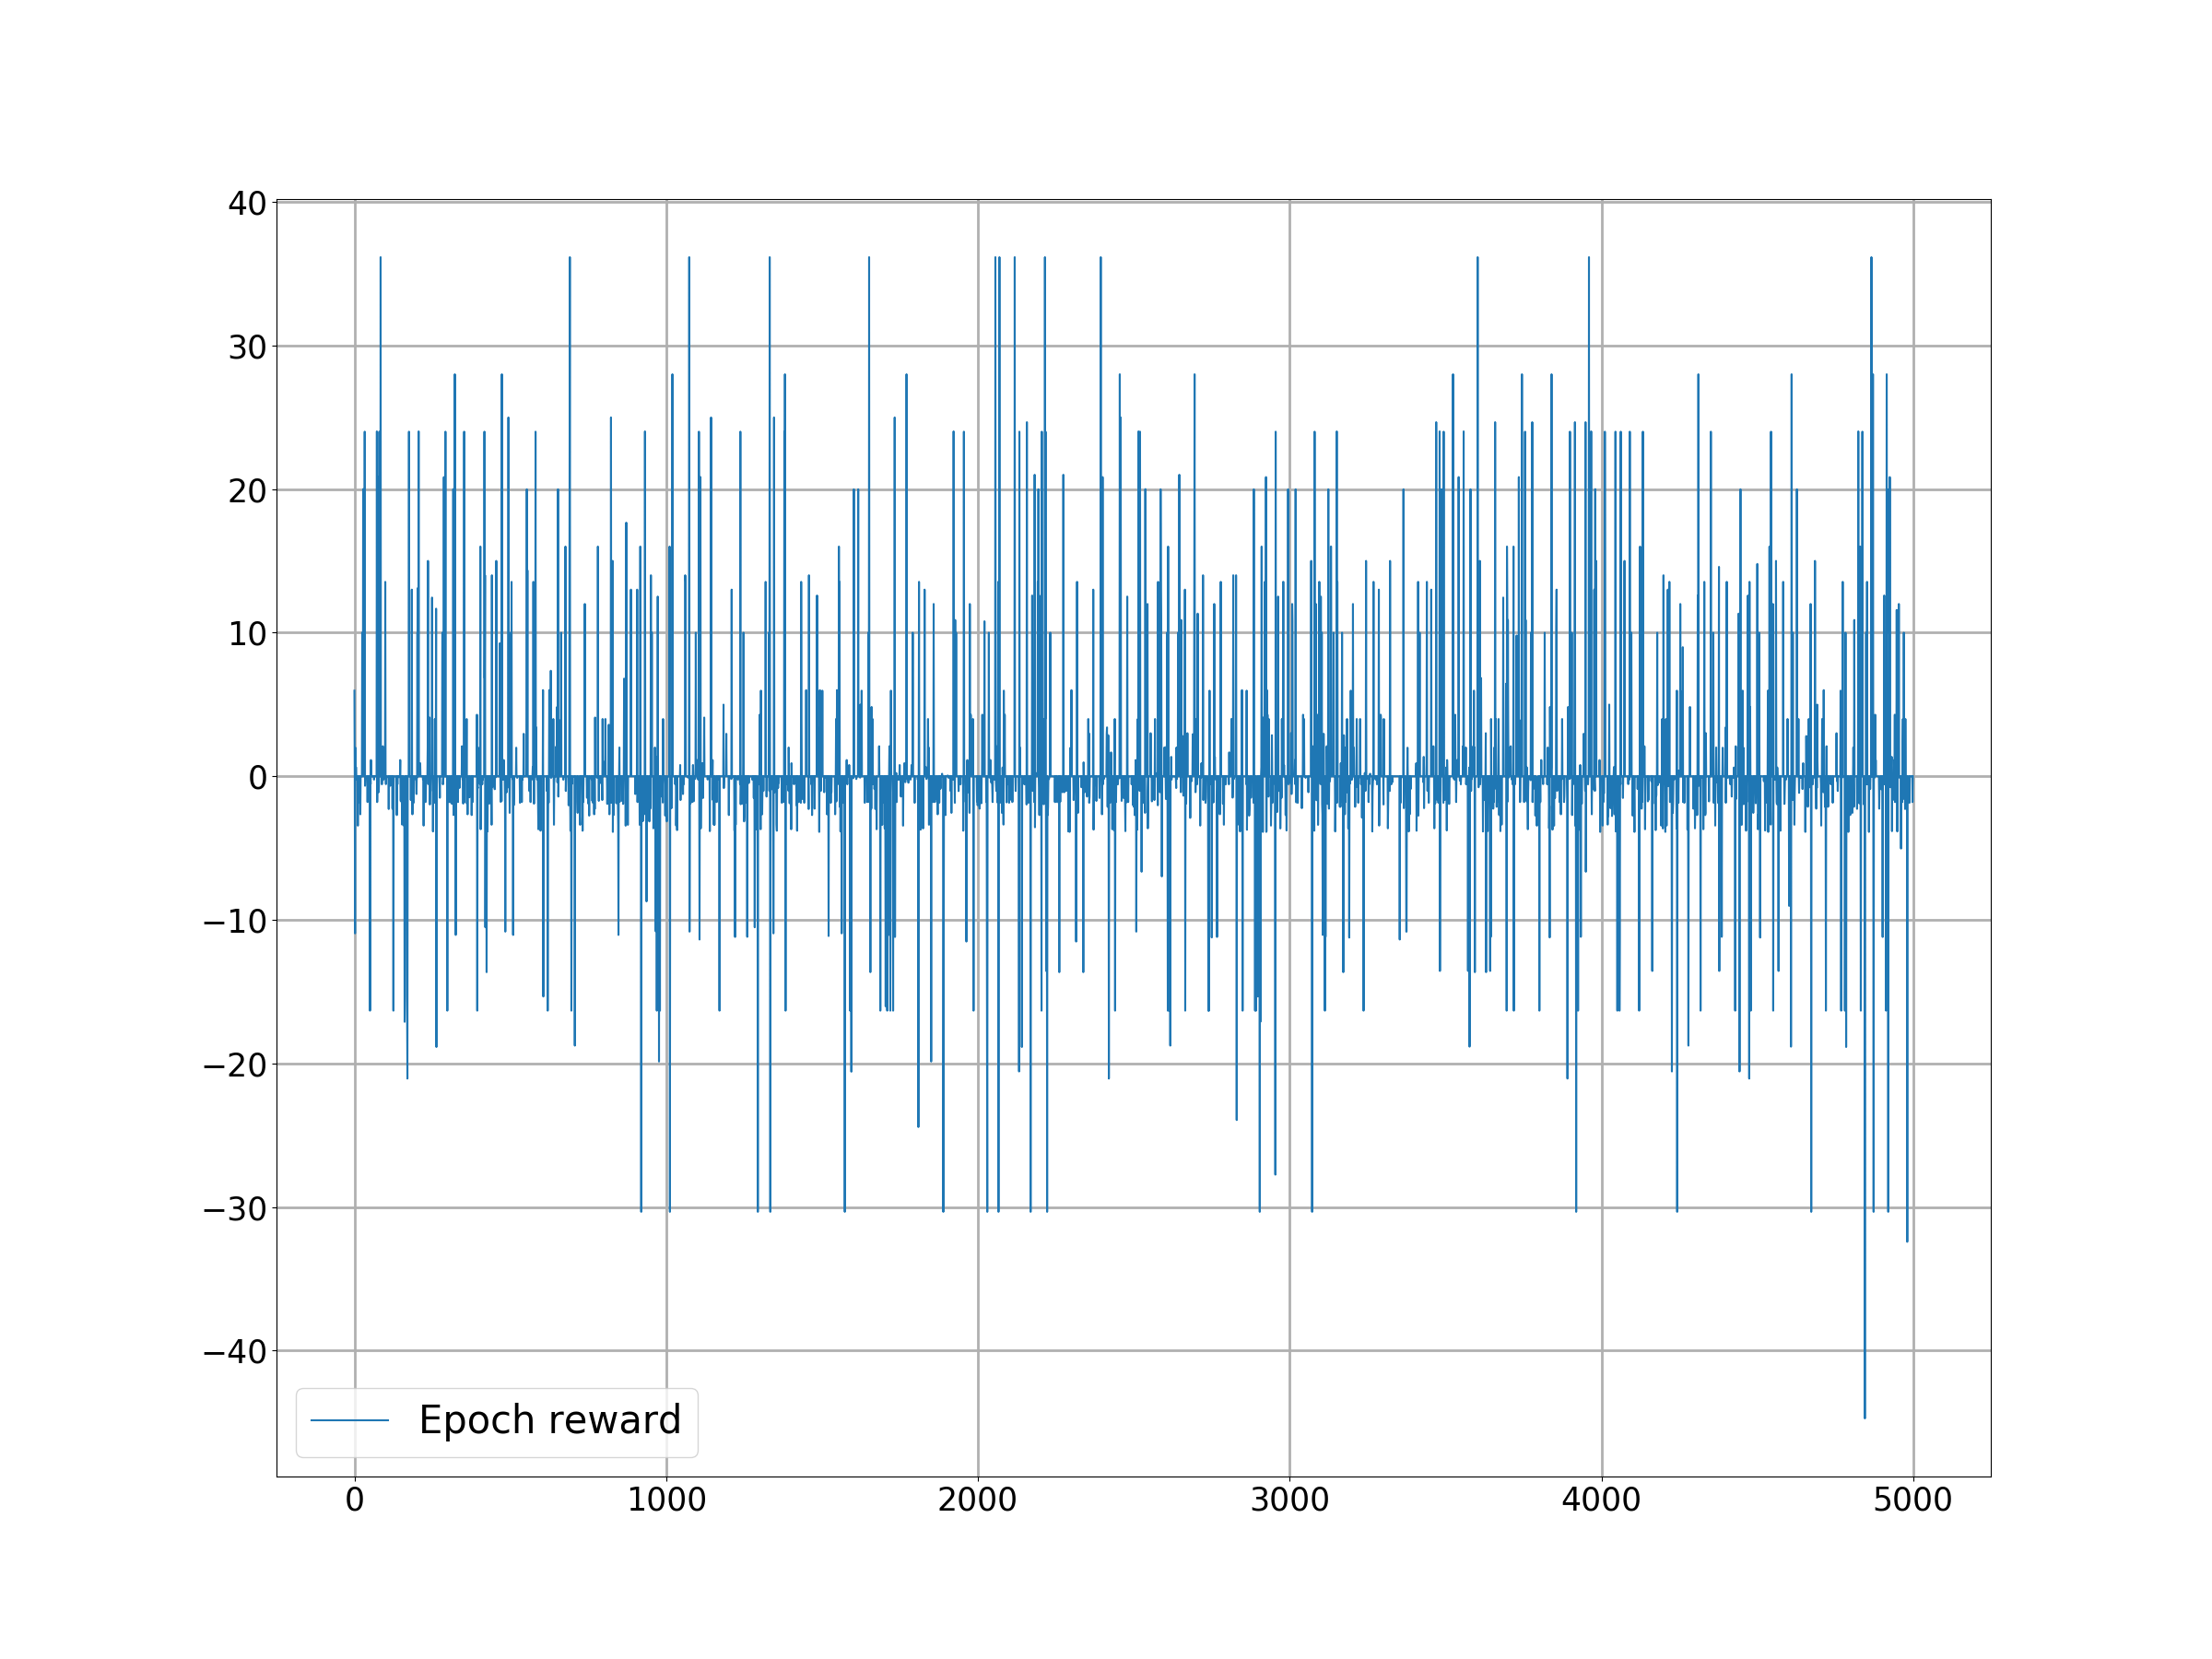
\includegraphics[width=\textwidth]{q_1_10000_BUY_rewards.png}
        \caption{Mean rewards per epoch (buy)}
        \label{fig:analysis-q-learn-1-reward-buy}
    \end{subfigure}
    \begin{subfigure}[b]{0.4\textwidth}
        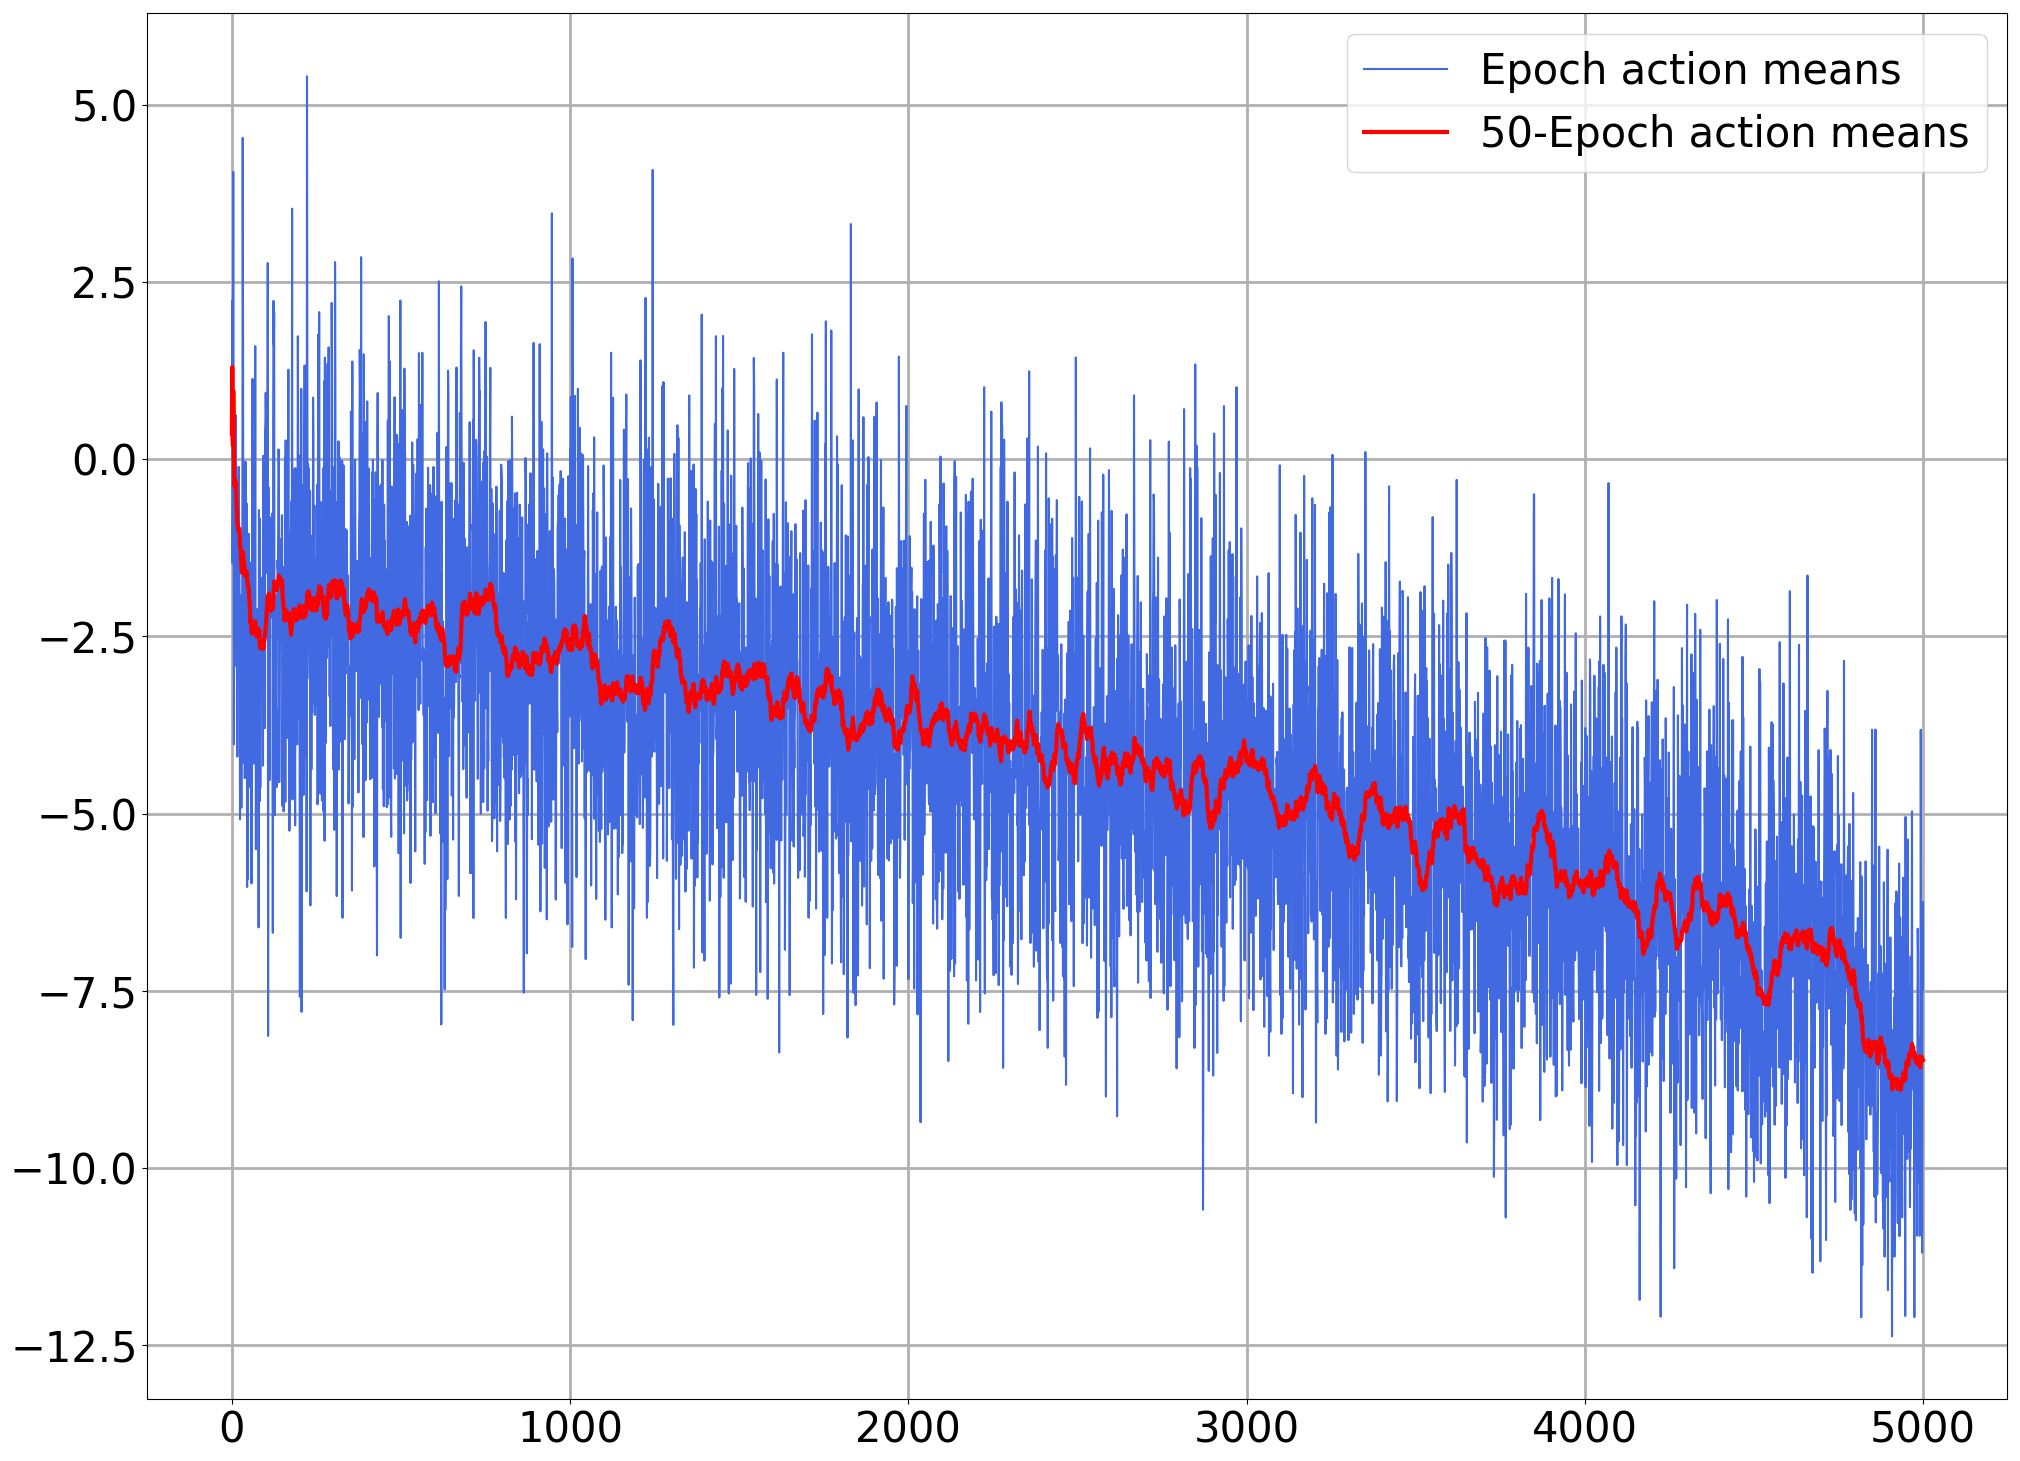
\includegraphics[width=\textwidth]{q_1_10000_BUY_mean_actions.png}
        \caption{Mean of actions per epoch (buy)}
        \label{fig:analysis-q-learn-1-action-buy}
    \end{subfigure}
    \begin{subfigure}[b]{0.4\textwidth}
        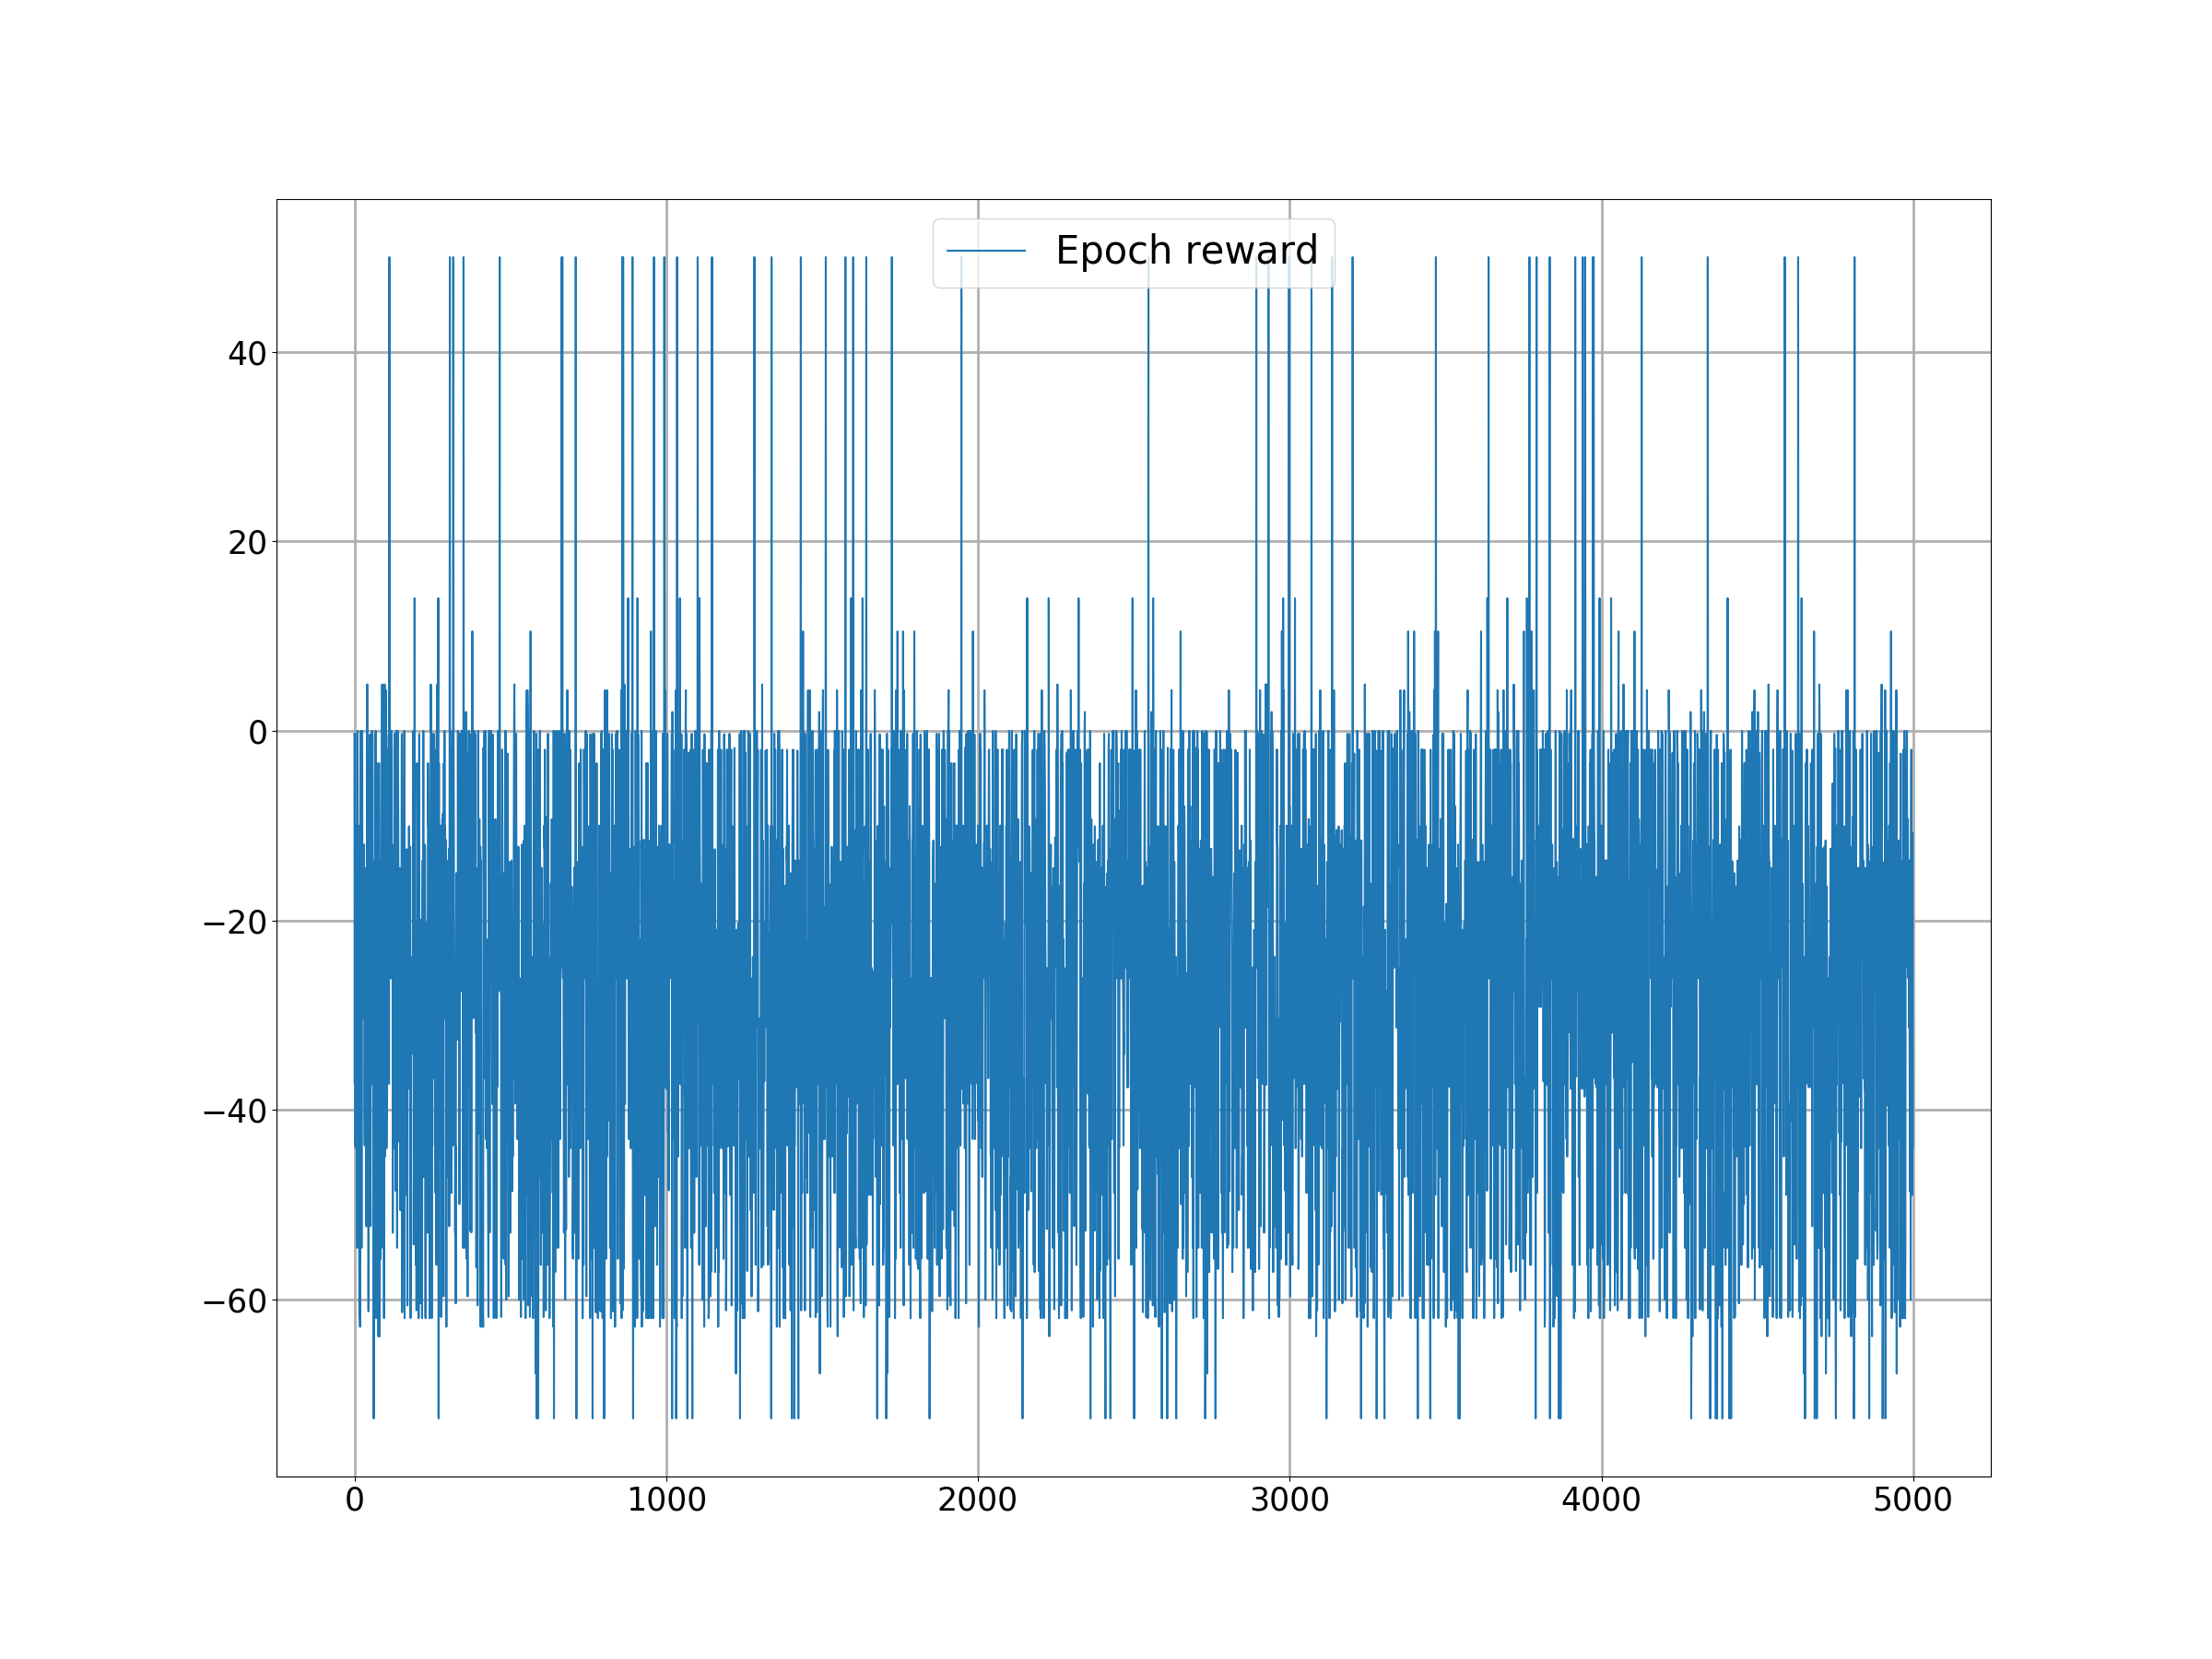
\includegraphics[width=\textwidth]{q_1_10000_SELL_rewards.png}
        \caption{Mean rewards per epoch (sell)}
        \label{fig:analysis-q-learn-1-reward-sell}
    \end{subfigure}
    \begin{subfigure}[b]{0.4\textwidth}
        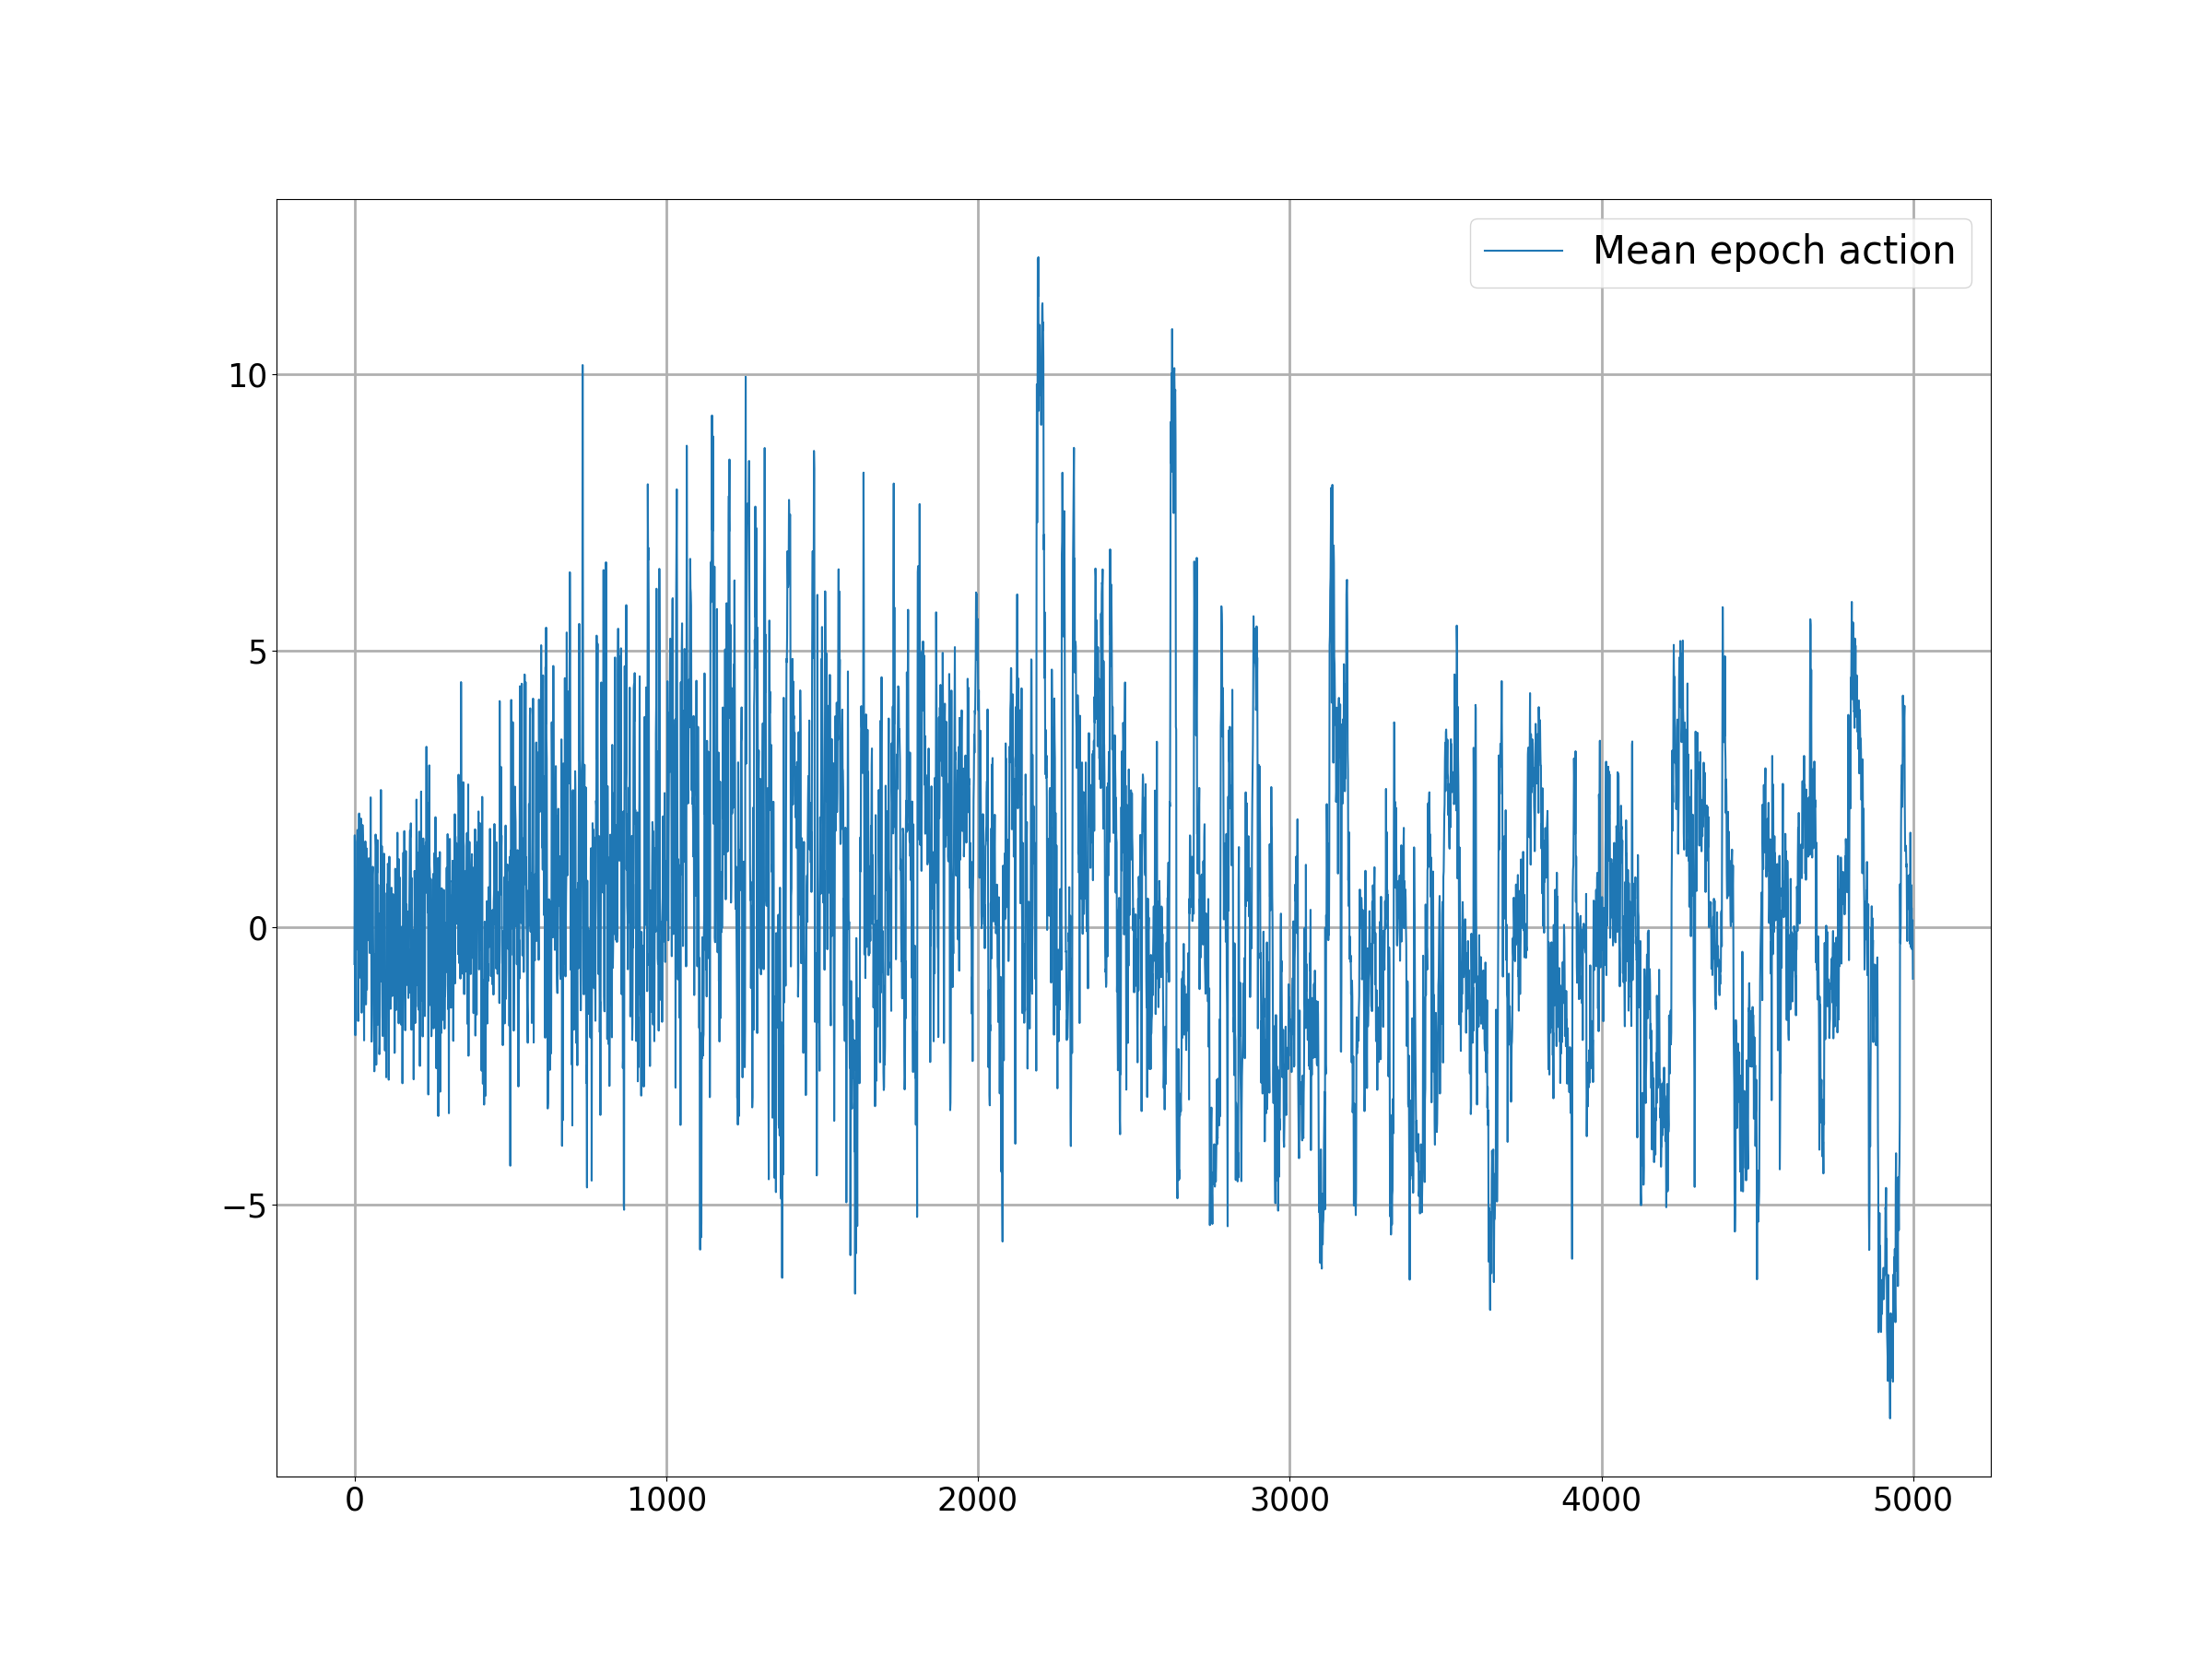
\includegraphics[width=\textwidth]{q_1_10000_SELL_mean_actions.png}
        \caption{Mean of actions per epoch (sell)}
        \label{fig:analysis-q-learn-1-action-sell}
    \end{subfigure}
    \caption{Mean rewards and actions for buying and selling on training data set I.}
    \label{fig:analysis-q-learn-1}
\end{figure}
\begin{figure}
    \centering
    \begin{subfigure}[b]{0.4\textwidth}
        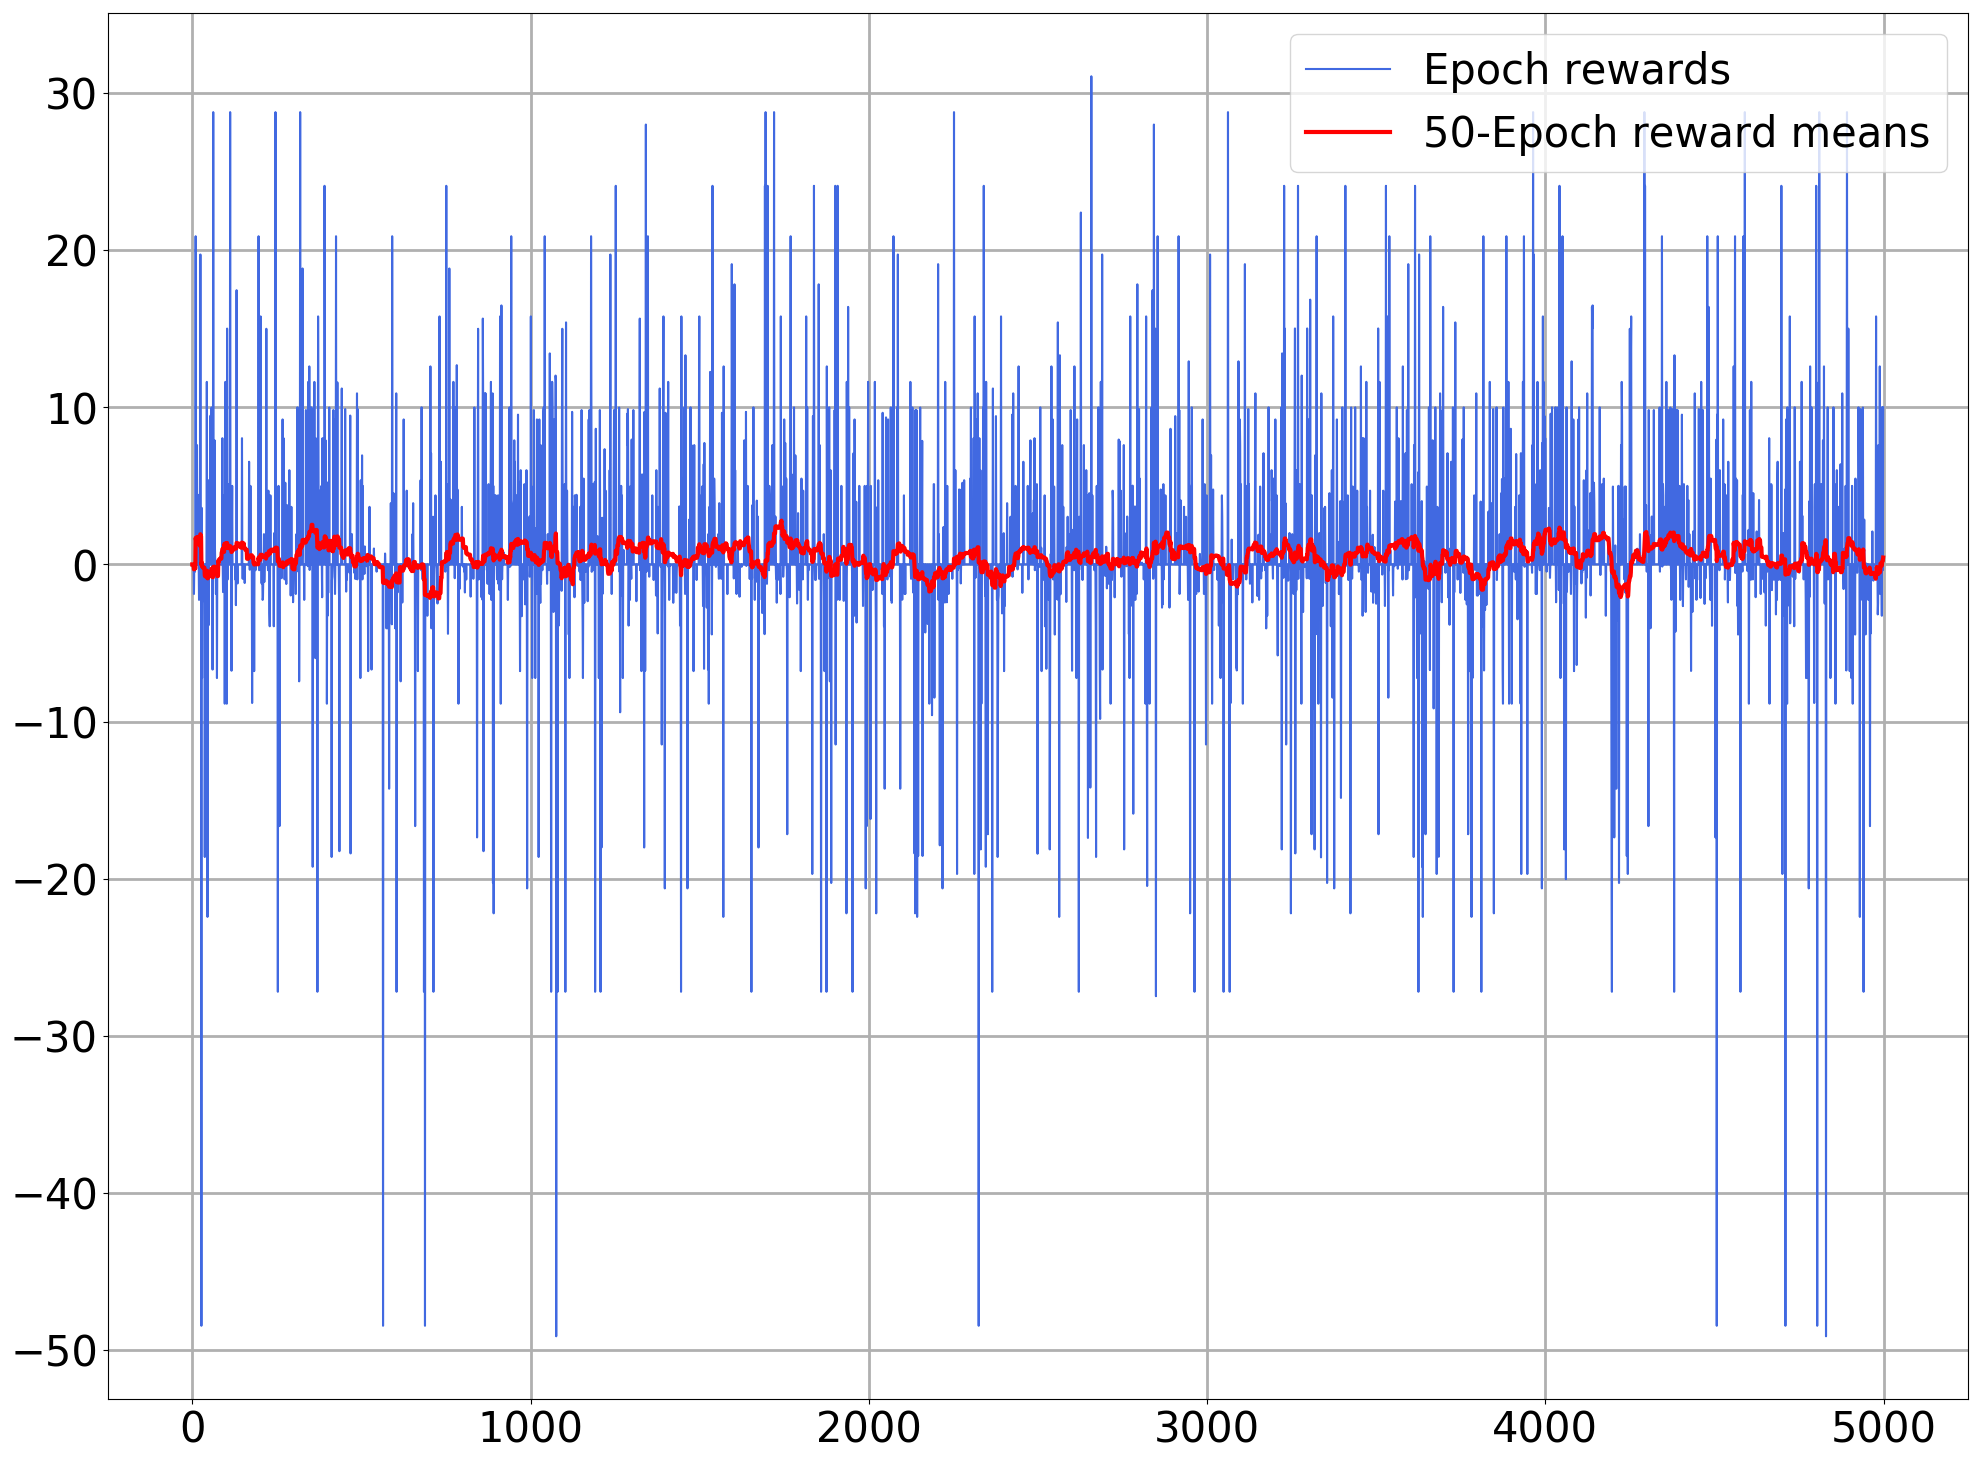
\includegraphics[width=\textwidth]{q_2_10000_BUY_rewards.png}
        \caption{Mean rewards per epoch (buy)}
        \label{fig:analysis-q-learn-2-reward-buy}
    \end{subfigure}
    \begin{subfigure}[b]{0.4\textwidth}
        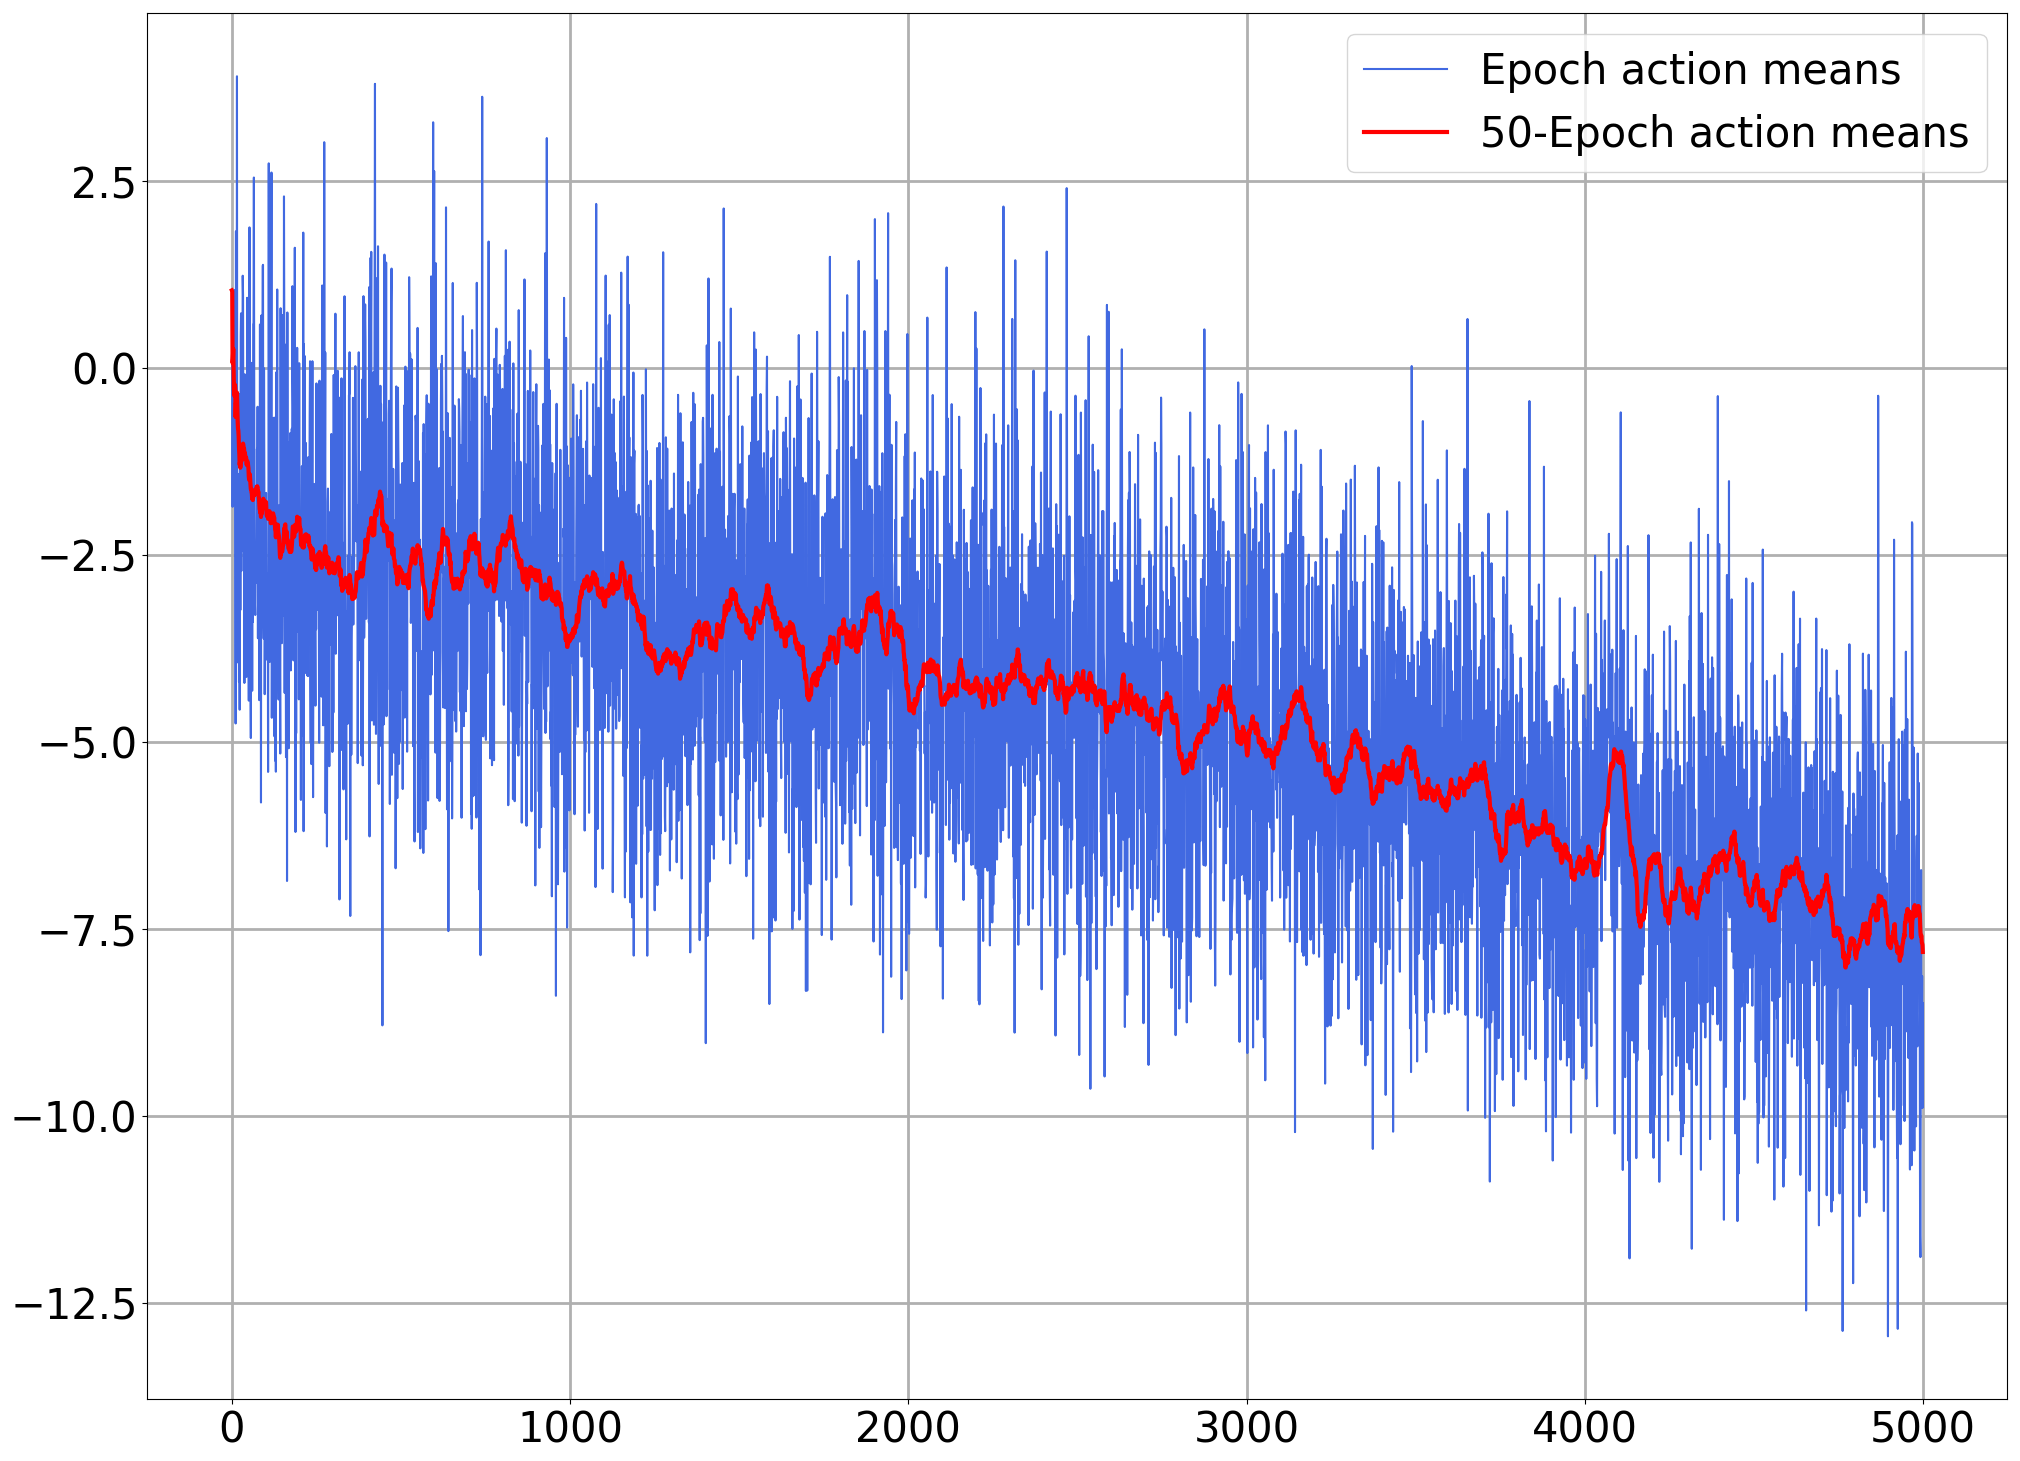
\includegraphics[width=\textwidth]{q_2_10000_BUY_mean_actions.png}
        \caption{Mean of actions per epoch (buy)}
        \label{fig:analysis-q-learn-2-action-buy}
    \end{subfigure}
    \begin{subfigure}[b]{0.4\textwidth}
        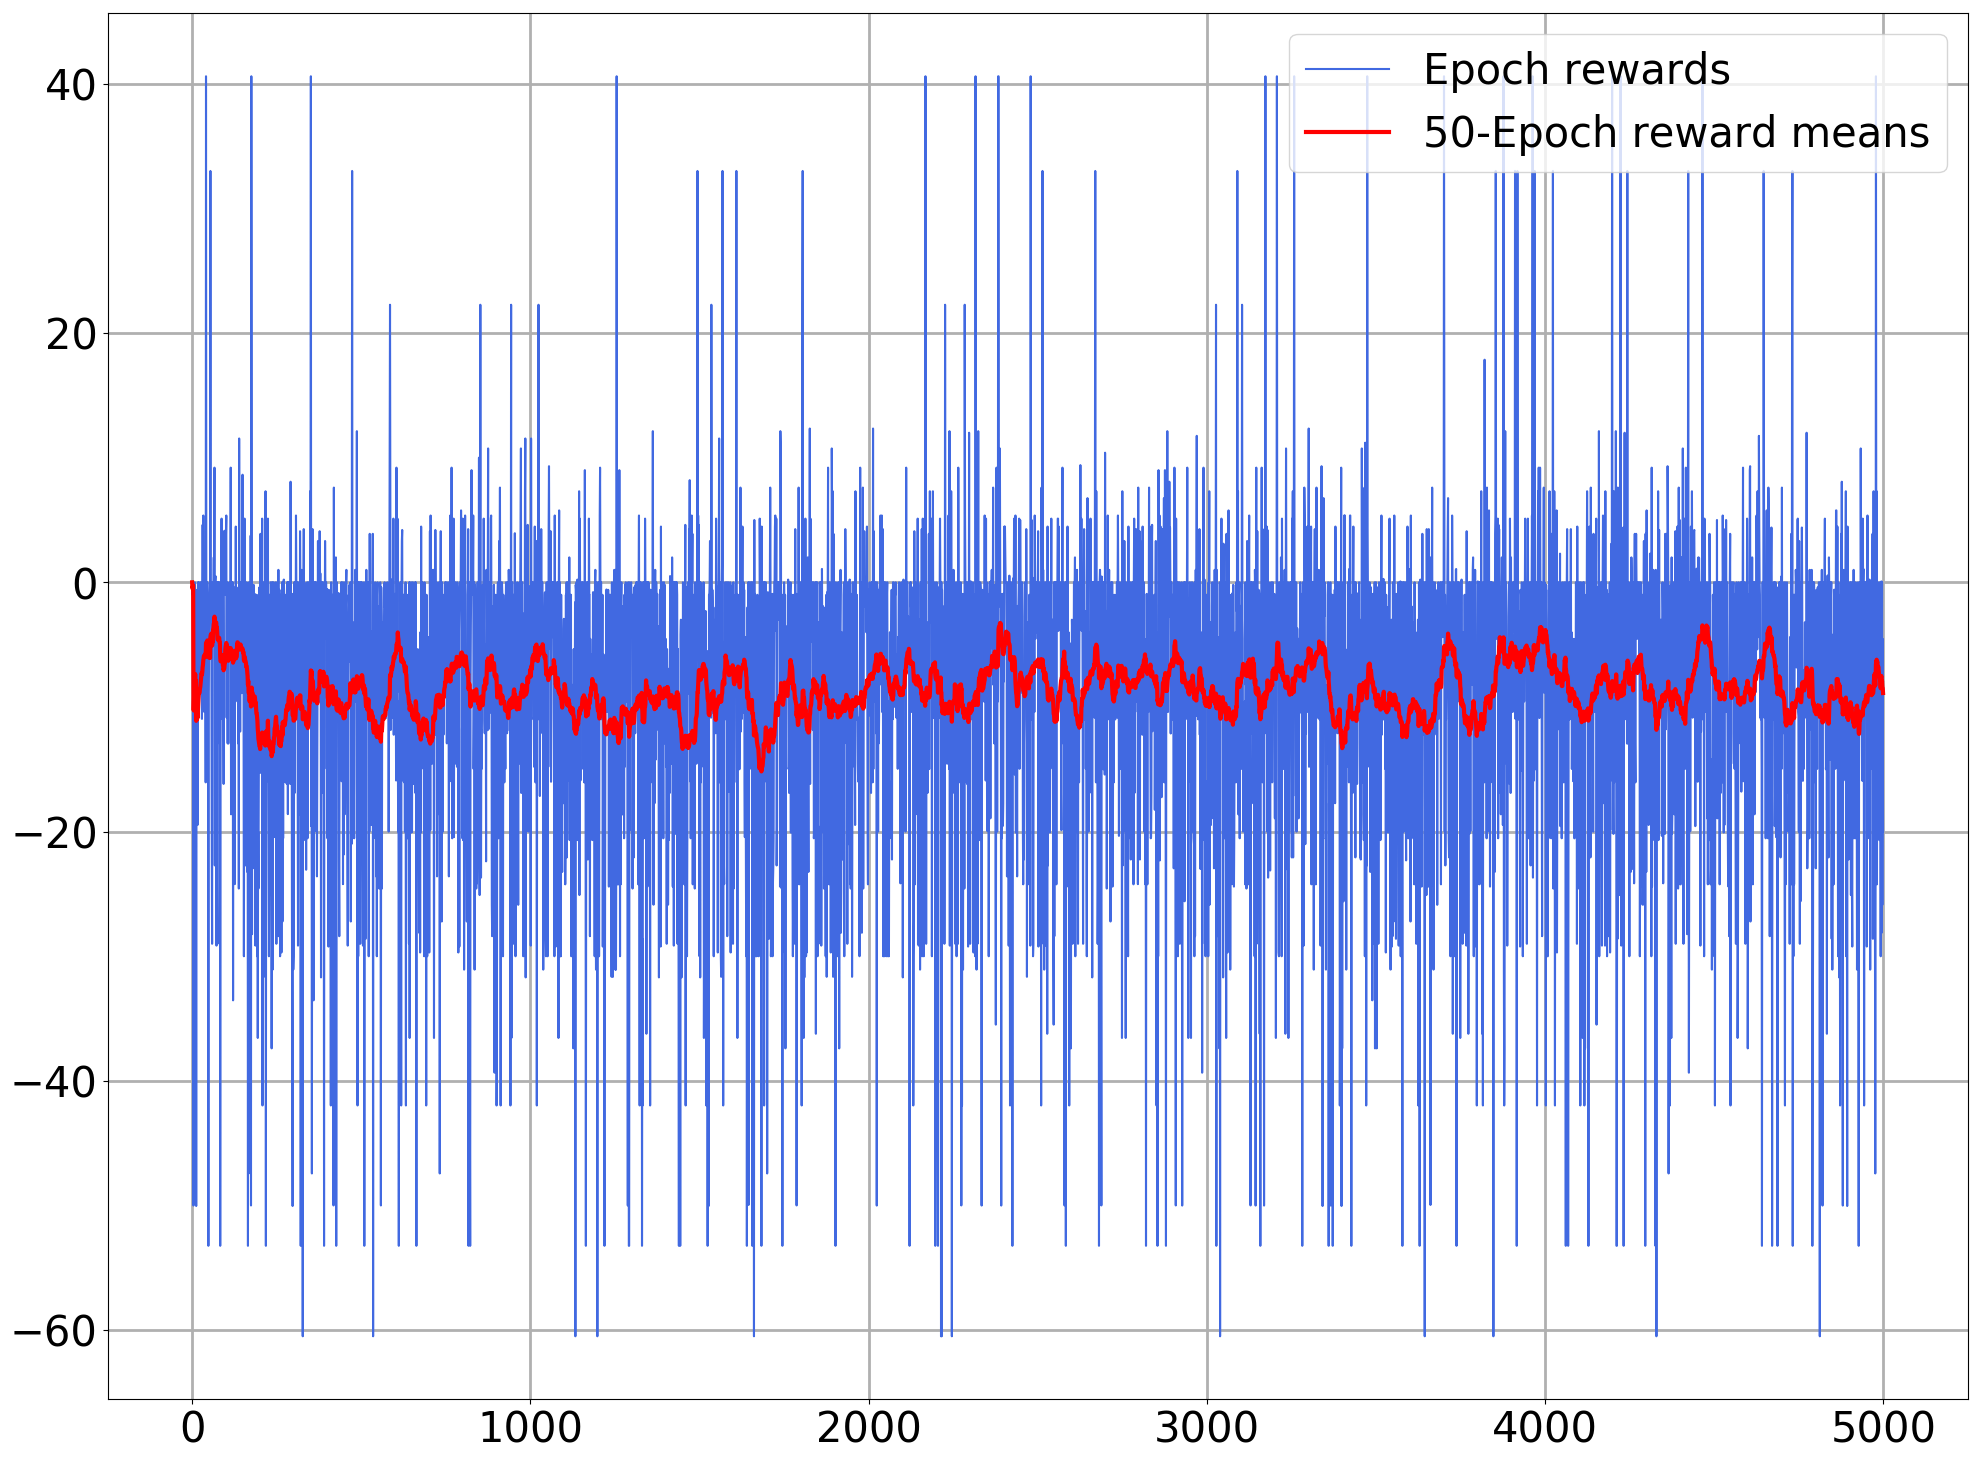
\includegraphics[width=\textwidth]{q_2_10000_SELL_rewards.png}
        \caption{Mean rewards per epoch (sell)}
        \label{fig:analysis-q-learn-2-reward-sell}
    \end{subfigure}
    \begin{subfigure}[b]{0.4\textwidth}
        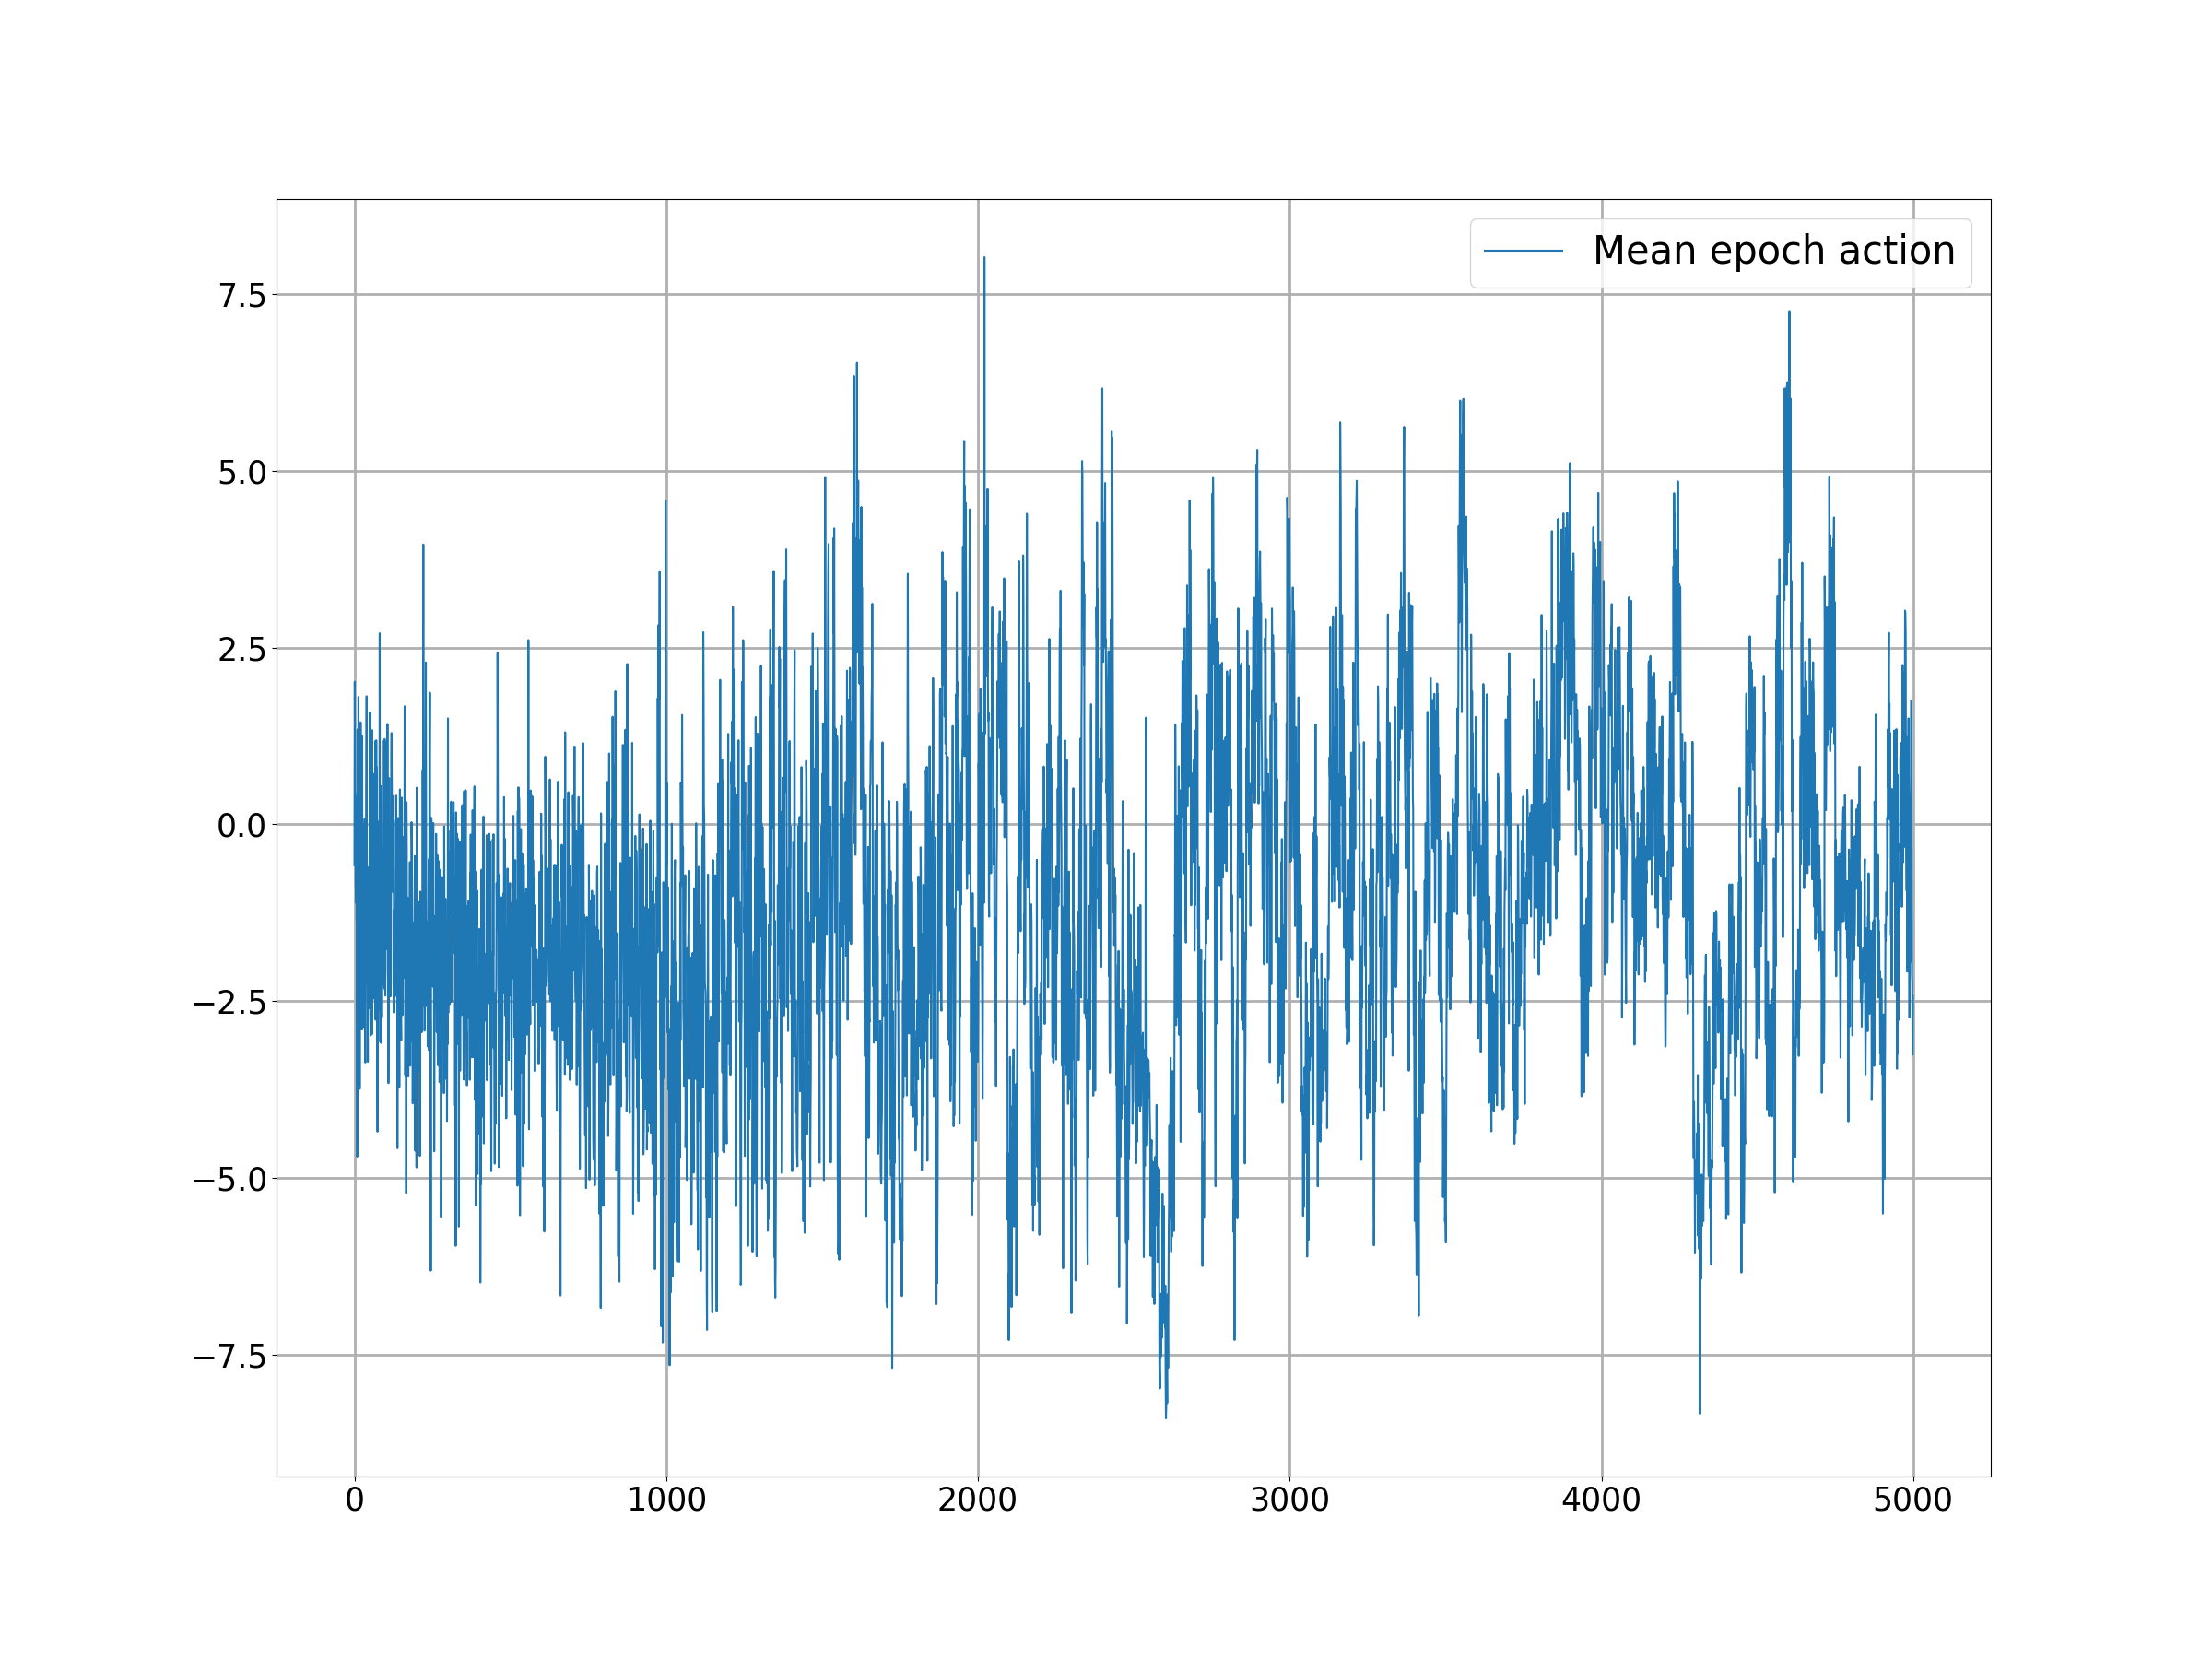
\includegraphics[width=\textwidth]{q_2_10000_SELL_mean_actions.png}
        \caption{Mean of actions per epoch (sell)}
        \label{fig:analysis-q-learn-2-action-sell}
    \end{subfigure}
    \caption{Mean rewards and actions for buying and selling on training data set II.}
    \label{fig:analysis-q-learn-2}
\end{figure}

Figure \ref{fig:analysis-q-learn-1} shows the experiment proceeded on data set I.
The average received reward during the training where the agents task was to buy 1.0 BTC within 100 seconds is shown in Figure \ref{fig:analysis-q-learn-1-reward-buy}.
Over the course of 5000 epochs, the agent was able to improve the mean reward slightly, by $\sim$0.5.
Reasons for this is the change in chosen actions as illustrated in Figure \ref{fig:analysis-q-learn-1-action-buy}.
The agent started off with an average action of $\sim$-3 which is a result of the low epsilon parameter that makes the agent choose actions randomly.
Actions where then adapted to the more negative side of the order book, such that after $\sim$1500 epochs the agent choose actions as low as -20 and then adjusted and stagnated at $\sim$-15.
The backtest, during which 1000 orders were executed on the test data set, resulted in an average reward of \textit{-1.17}--that is worse than the average reward received on the training close to the end of the training.
The cost of a market order on the test data set is -0.05 such that the strategy of the agent results in additional costs of \$-1.12 when buying 1.0 BTC.
Comparing the found results to the empirical analysis proceeded on the same data set, as shown in Figure \ref{fig:behvaiour-down}, provides means for interpretation:
Considering the backtest results and the highly negative average action the agent chooses towards the end of the training indicates that the order was oftentimes not able to be filled within the time horizon and a market order was followed.

The rewards received for the agents tasks to sell the assets are much more volatile, as shown in Figure \ref{fig:analysis-q-learn-1-reward-sell}, and no clear improvement can be seen.
Consequently, there was no significant adjustment made by the agent regarding the chosen actions, as indicated in Figure \ref{fig:analysis-q-learn-1-action-sell}.
The agent started off at limit level 0 and after some exploration concluded to keep choosing actions at the same level as it started off.
The backtest resulted in an average reward of -21.34 achieved by the agent.
The reward received for placing market orders on the test set account to a negative reward of -27.70.
Hence, the agent is able to save \$6.36 when selling 1.0 BTC.
\\
\\
Figure \ref{fig:analysis-q-learn-2} shows the experiment proceeded on data set II.
The average received reward while training to buy the asset is shown in Figure \ref{fig:analysis-q-learn-2-reward-buy}.
Throughout the epochs, the agent was able to improve the mean reward like with the previous data by roughly 0.5.
Even though the trend of this data set is the opposite, the change in chosen actions correlates to the previous findings and is illustrated in Figure \ref{fig:analysis-q-learn-2-action-buy}.
The backtest on the test data set (of data set II), resulted in an average reward of \textit{-1.04} -- again worse than the average reward received on the training set.
A market order on this test data accounts to an average reward of -1.06, indicating that the agent is saving \$0.02 when buying 1.0 BTC.
When taking the empirical analysis proceeded on this data set into consideration, as shown in Figure \ref{fig:behvaiour-up}, the received rewards indicate that the agent again failed to execute orders with the placed limit orders and oftentimes market orders followed.

Similar to the order placed on data set I, the rewards received for the agents tasks to sell the assets are much more volatile when it comes to selling, as shown in Figure \ref{fig:analysis-q-learn-1-reward-sell}.
No improvement can be seen from the rewards during the training as no significant adjustment was made by the agent regarding the chosen actions, as indicated in Figure \ref{fig:analysis-q-learn-2-action-sell}.
The backtest resulted in an average reward of -4.74 achieved by the agent, whereas market orders result to an average reward of -1.72.
Hence, the agent causes to pay a premium of \$3.02 for selling 1.0 BTC.

\subsection{Conclusion of Q-Learning approach}

\begin{table}[H]
\centering
\begin{tabular}{l|l|l|}
\cline{2-3}
& \textbf{Agent} & \textbf{\begin{tabular}[c]{@{}l@{}}Market\\ Order\end{tabular}} \\ \hline
\multicolumn{1}{|l|}{\textbf{Buy (I)}}   & -1.17          & -0.05                                                           \\ \hline
\multicolumn{1}{|l|}{\textbf{Sell (I)}}  & -21.34         & -27.70                                                          \\ \hline
\multicolumn{1}{|l|}{\textbf{Buy (II)}}  & -1.04          & -1.06                                                           \\ \hline
\multicolumn{1}{|l|}{\textbf{Sell (II)}} & -4.74          & -1.72                                                           \\ \hline
\end{tabular}
\caption{Summary of rewards for the Q-Learning agent and market orders.}
\label{tbl:analysis-q-learn-summary}
\end{table}
The findings of this section are summarized in Table \ref{tbl:analysis-q-learn-summary}.
We conclude that the Q-Learning agent was not able to place buy and sell orders in a way which would result in a price better than the current market price.
Oftentimes, a market order which would cause an immediate buy or sell would even be the better choice.
Clearly, this is due to the fact that the agent was not able to find the most suitable actions.
Furthermore, in order to investigate whether or not these results were a result of the agent aiming for too much immediate reward, the same experiment was proceeded with $\gamma=0.3$.
However, no improvement could be made and instead the agent achieved similar results while requiring more epochs in order to converge to the same mean of actions.
In this section we have only investigated the mean of the actions chosen throughout an epoch, which gave enough proofs that the chosen actions resulted mostly in market orders.
In the following section, where the DQN agent is being investigated, we plan to investigate the chosen sequence of actions within one epoch in order to gain even better understanding about the decision process of the agent.
Furthermore, it is to be assumed that the absence of market variables, while only relying on the given rewards, makes it hard for any learner to determine an optimal strategy.
Therefore, the following section will make use of market variables in order to determine whether or not a learner can exploit the information hidden in the market and then act in favour of optimally placing limit orders.

\section{Deep Q-Network}
\label{sec:eval-dqn}
In the previous section the Q-Learning agent was trained on the given data sets and no significant optimization in terms of buying and selling assets was achieved.
That was, without market variables and by only relying on private variables instead.
By considering the previously found results of the empirical analysis of the limit order placement behaviour we found that most of the limit orders placed by the Q-Learning agent were not filled within the given time horizon and instead market orders had to be submitted after the time was consumed.

In this section we aim to determine whether or not the DQN agent is capable of extracting information provided by the raw market features and therefore improve the limit order placement strategy.
The setup is the same as in the previous section whereas the agents task is to buy and sell 1.0 BTC within 100 seconds (step size 10 seconds) on both data sets I and II.
Furthermore, both features which were derived in Chapter \ref{chap:data} will be applied and investigated separately.
We then reason about the capabilities of this approach in greater detail by investigating a sample order submission and uncover the actions the agent chooses to take throughout one epoch.
In addition, artificial order books are being created which serve as new data sets to train and test the DQN agent on.
By doing so, we aim to determine the limitations of this approach.
Finally, we conclude our findings and reason about the capabilities of the DQN approach (and its use of the market features) by comparing it to the previously stated Q-Learning results.

\subsection{Application of historical order feature}


\begin{figure}[H]
    \centering
    \begin{subfigure}[b]{0.45\textwidth}
        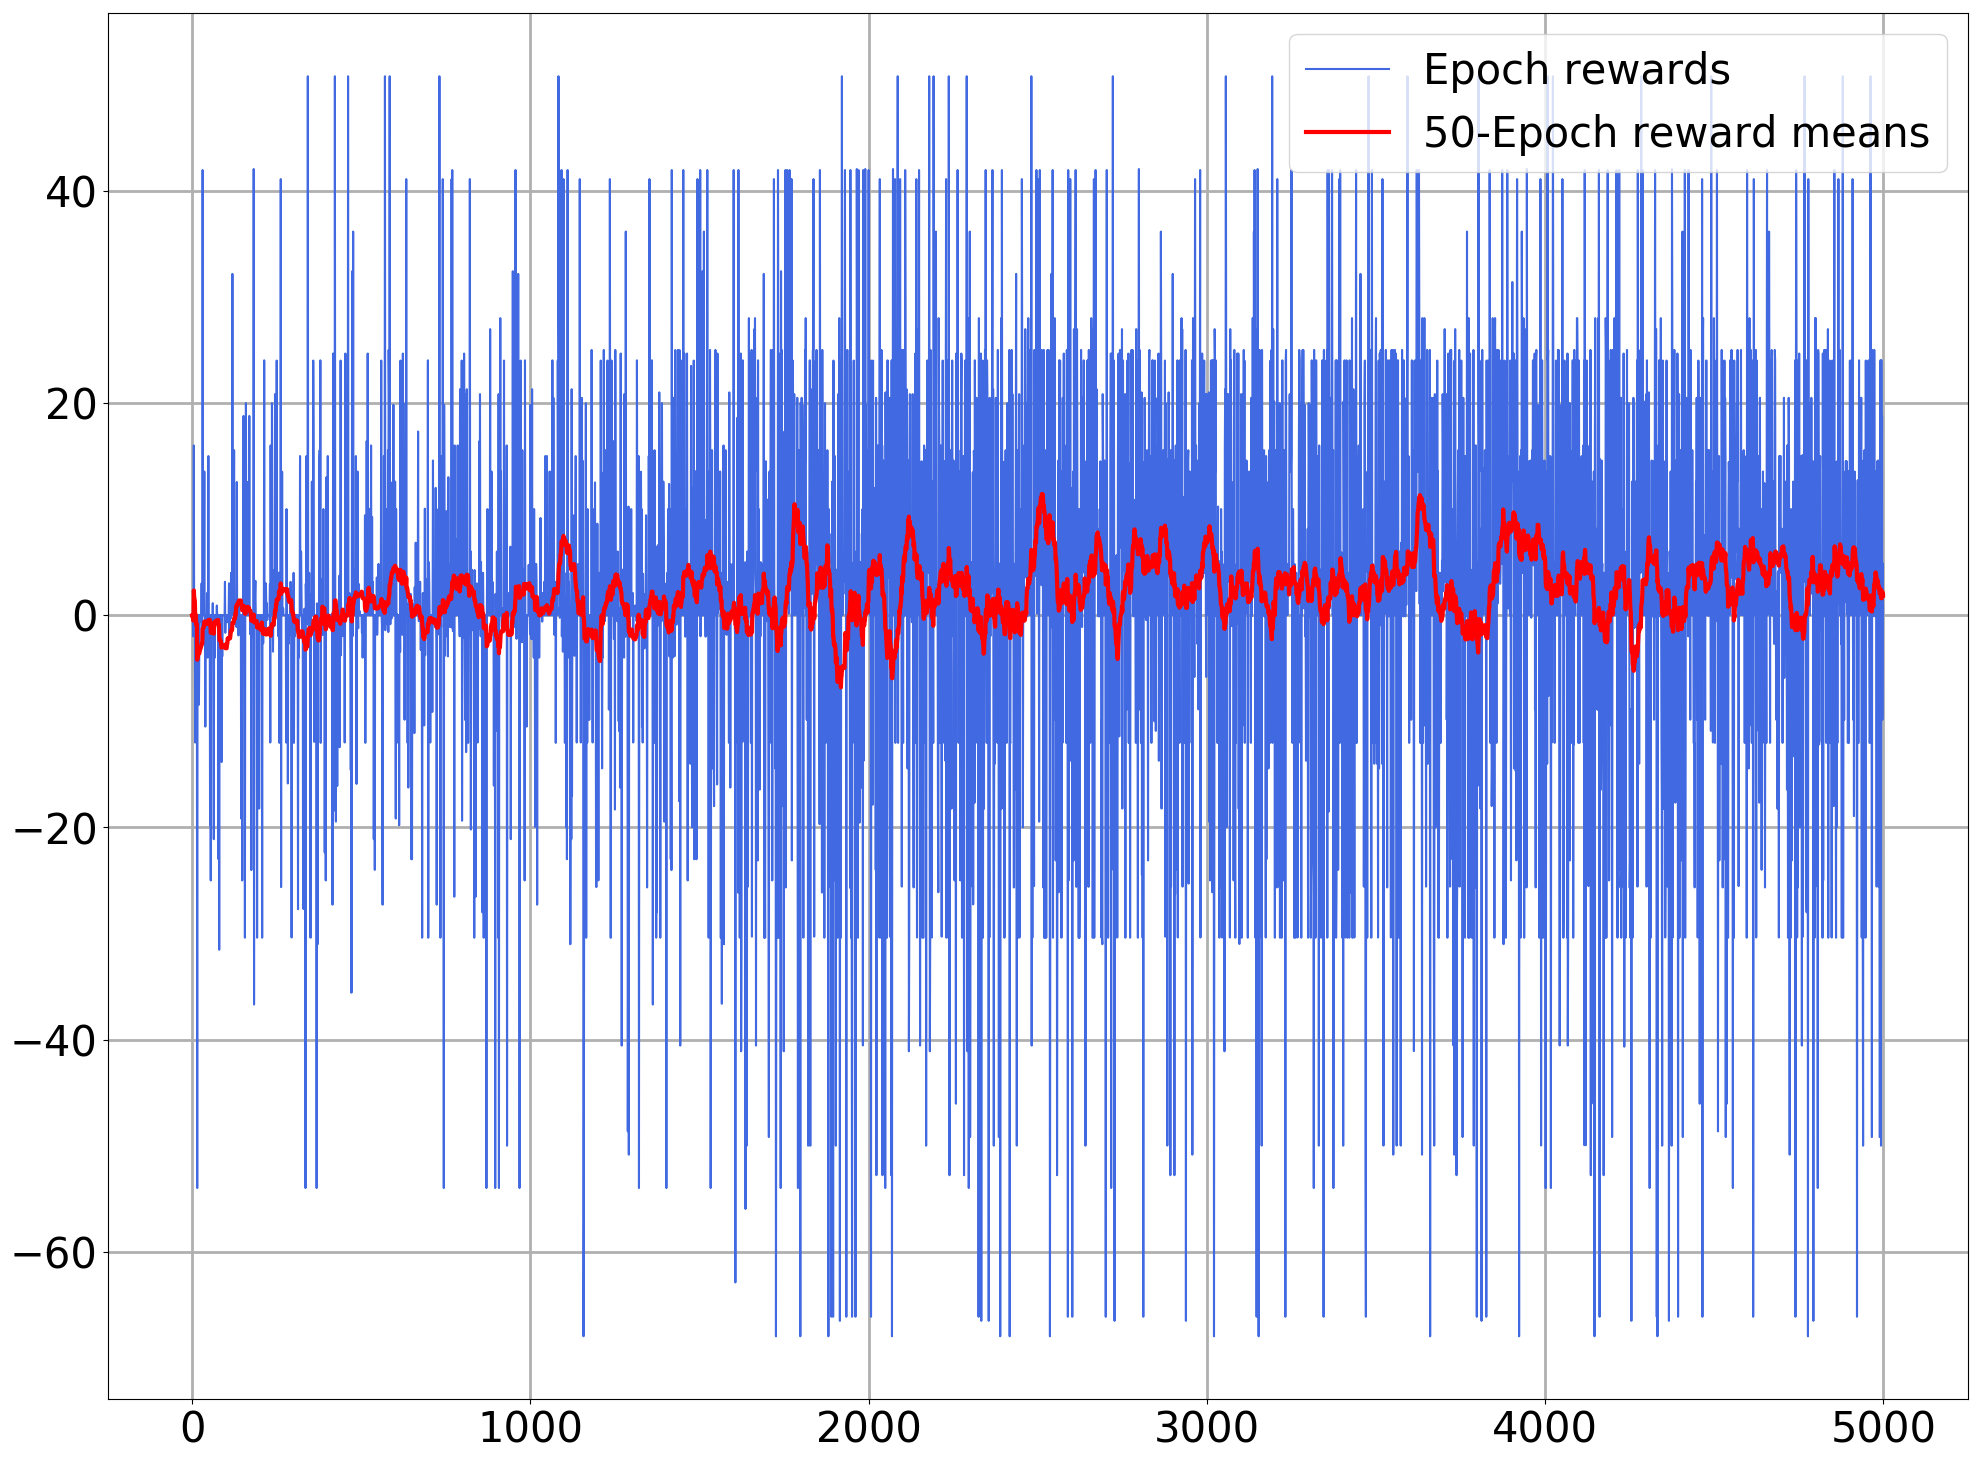
\includegraphics[width=\textwidth]{cnn_1_buy_rewards.png}
        \caption{Reward per epoch (buy)}
        \label{fig:analysis-dqn-1-reward-buy}
    \end{subfigure}
    \begin{subfigure}[b]{0.45\textwidth}
        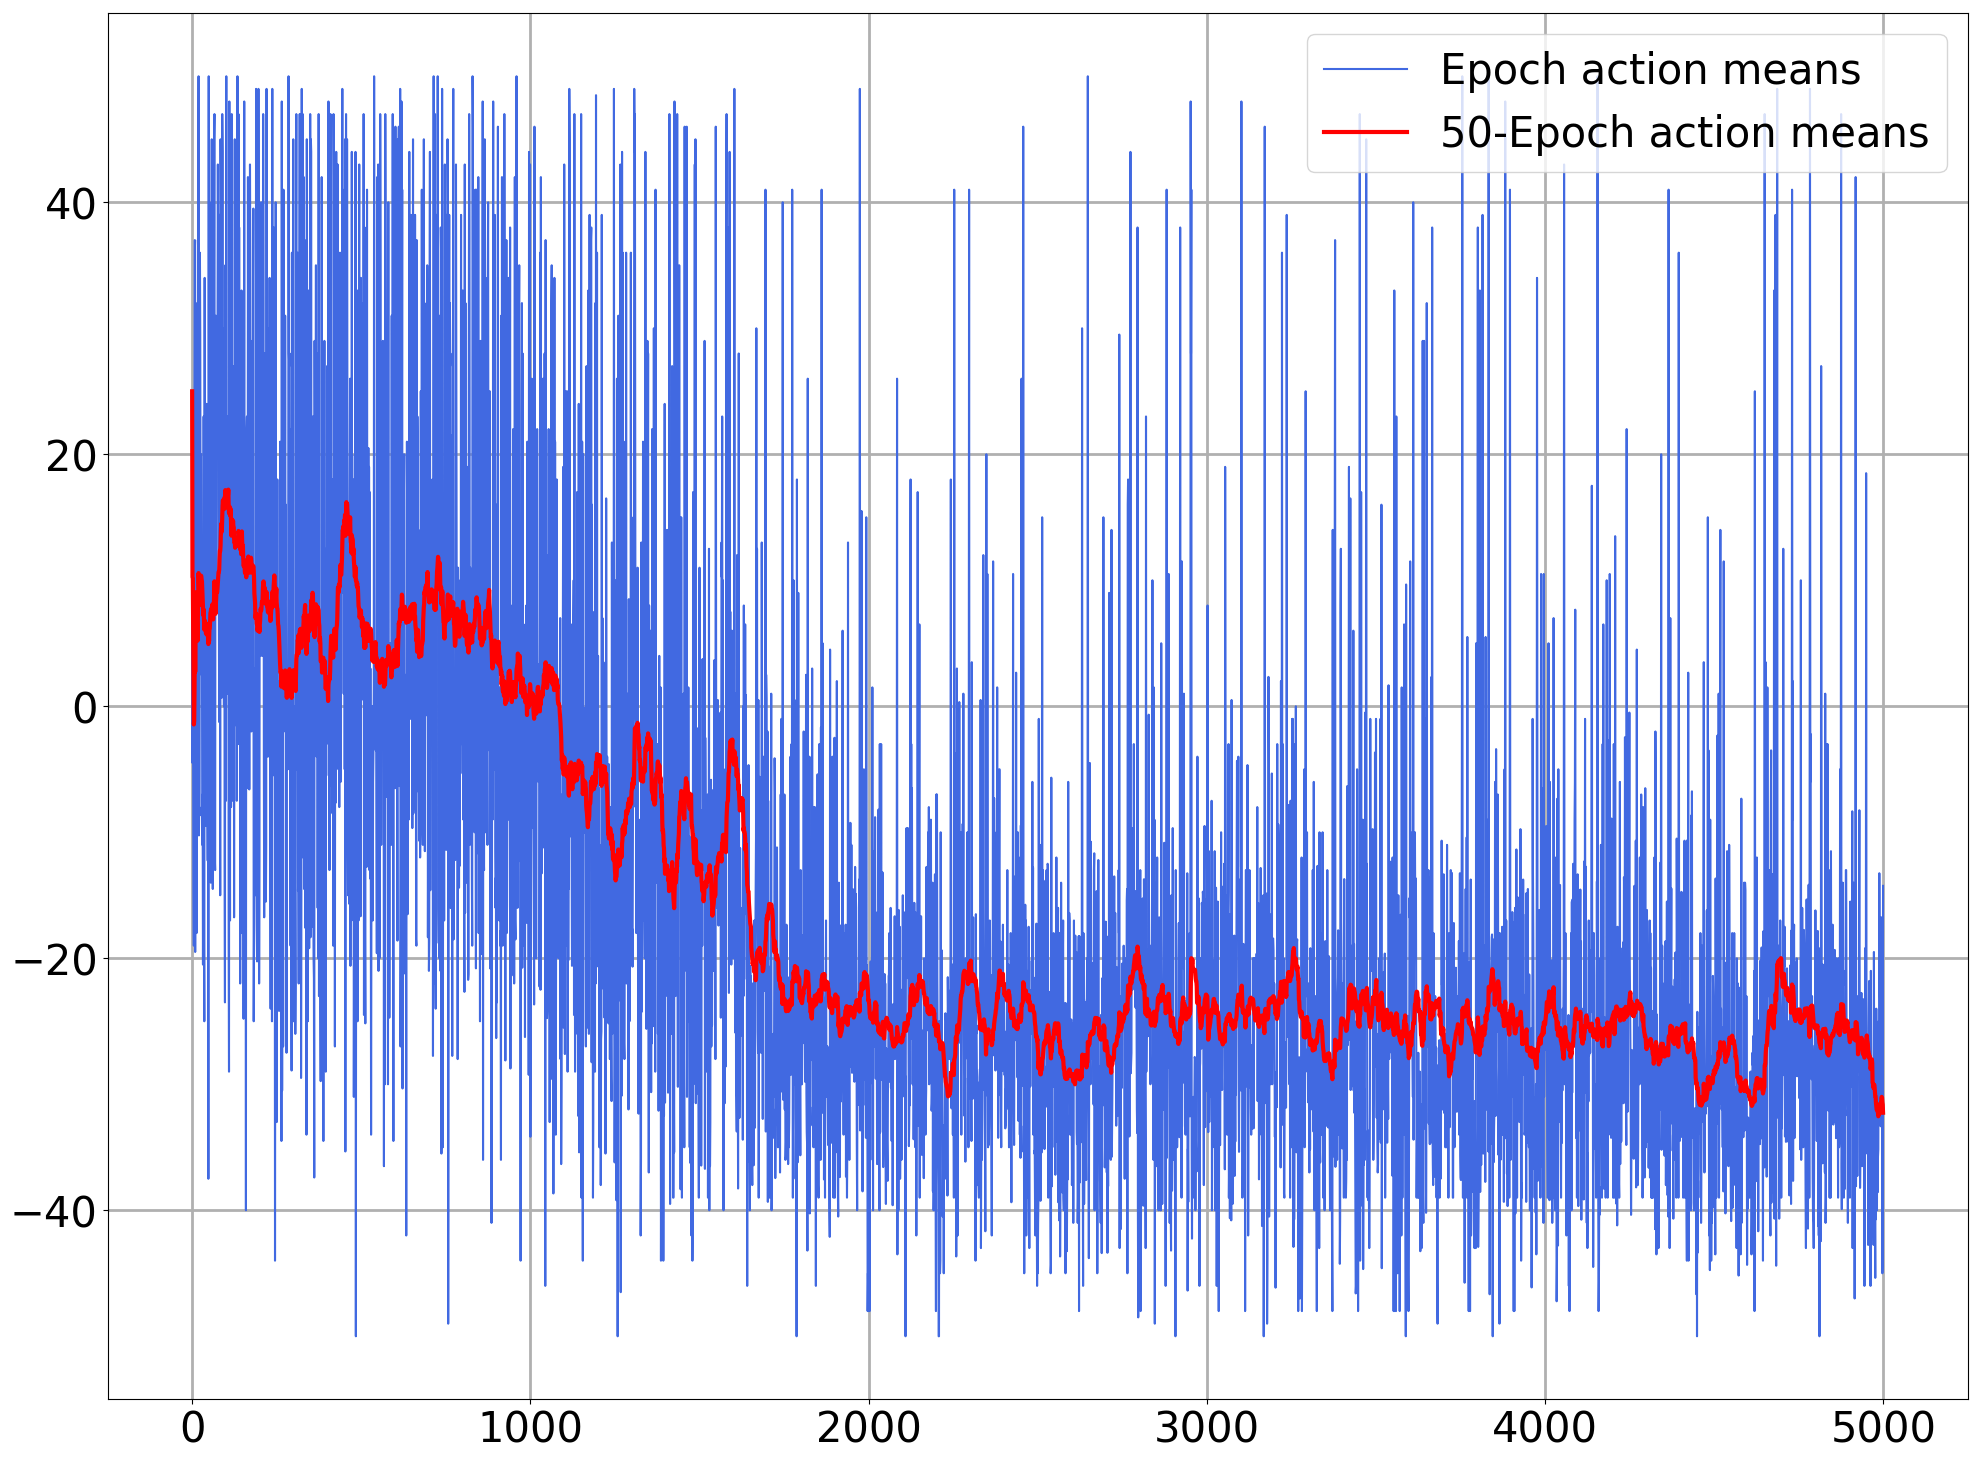
\includegraphics[width=\textwidth]{cnn_1_buy_mean_actions.png}
        \caption{Mean of actions per epoch (buy)}
        \label{fig:analysis-dqn-1-action-buy}
    \end{subfigure}
    \begin{subfigure}[b]{0.45\textwidth}
        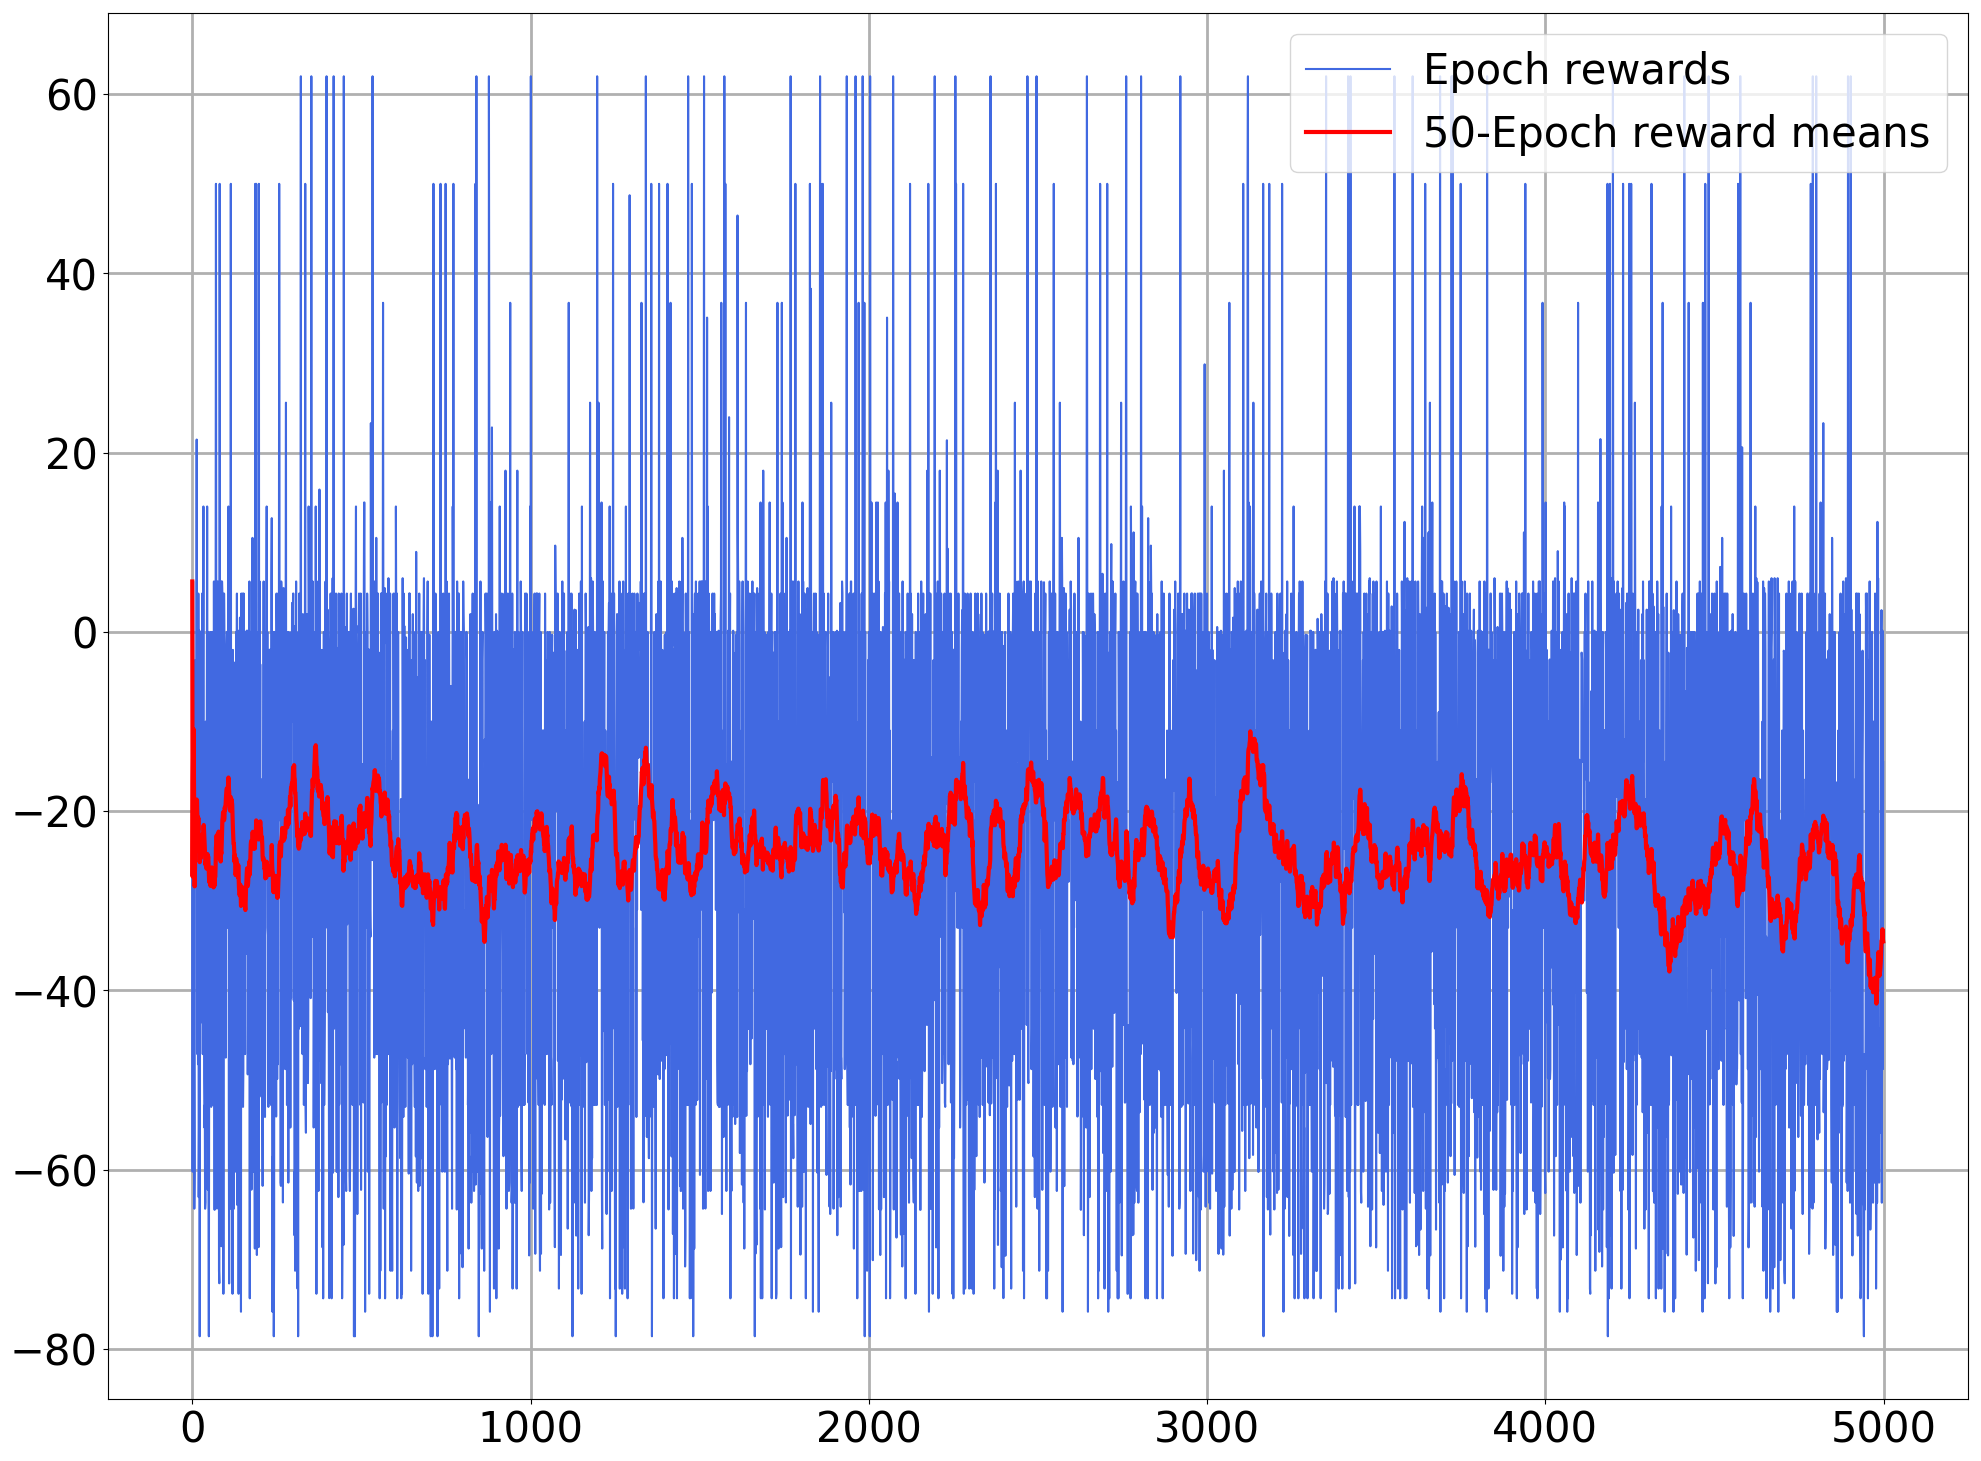
\includegraphics[width=\textwidth]{cnn_1_sell_rewards.png}
        \caption{Mean rewards per epoch (sell)}
        \label{fig:analysis-dqn-1-reward-sell}
    \end{subfigure}
    \begin{subfigure}[b]{0.45\textwidth}
        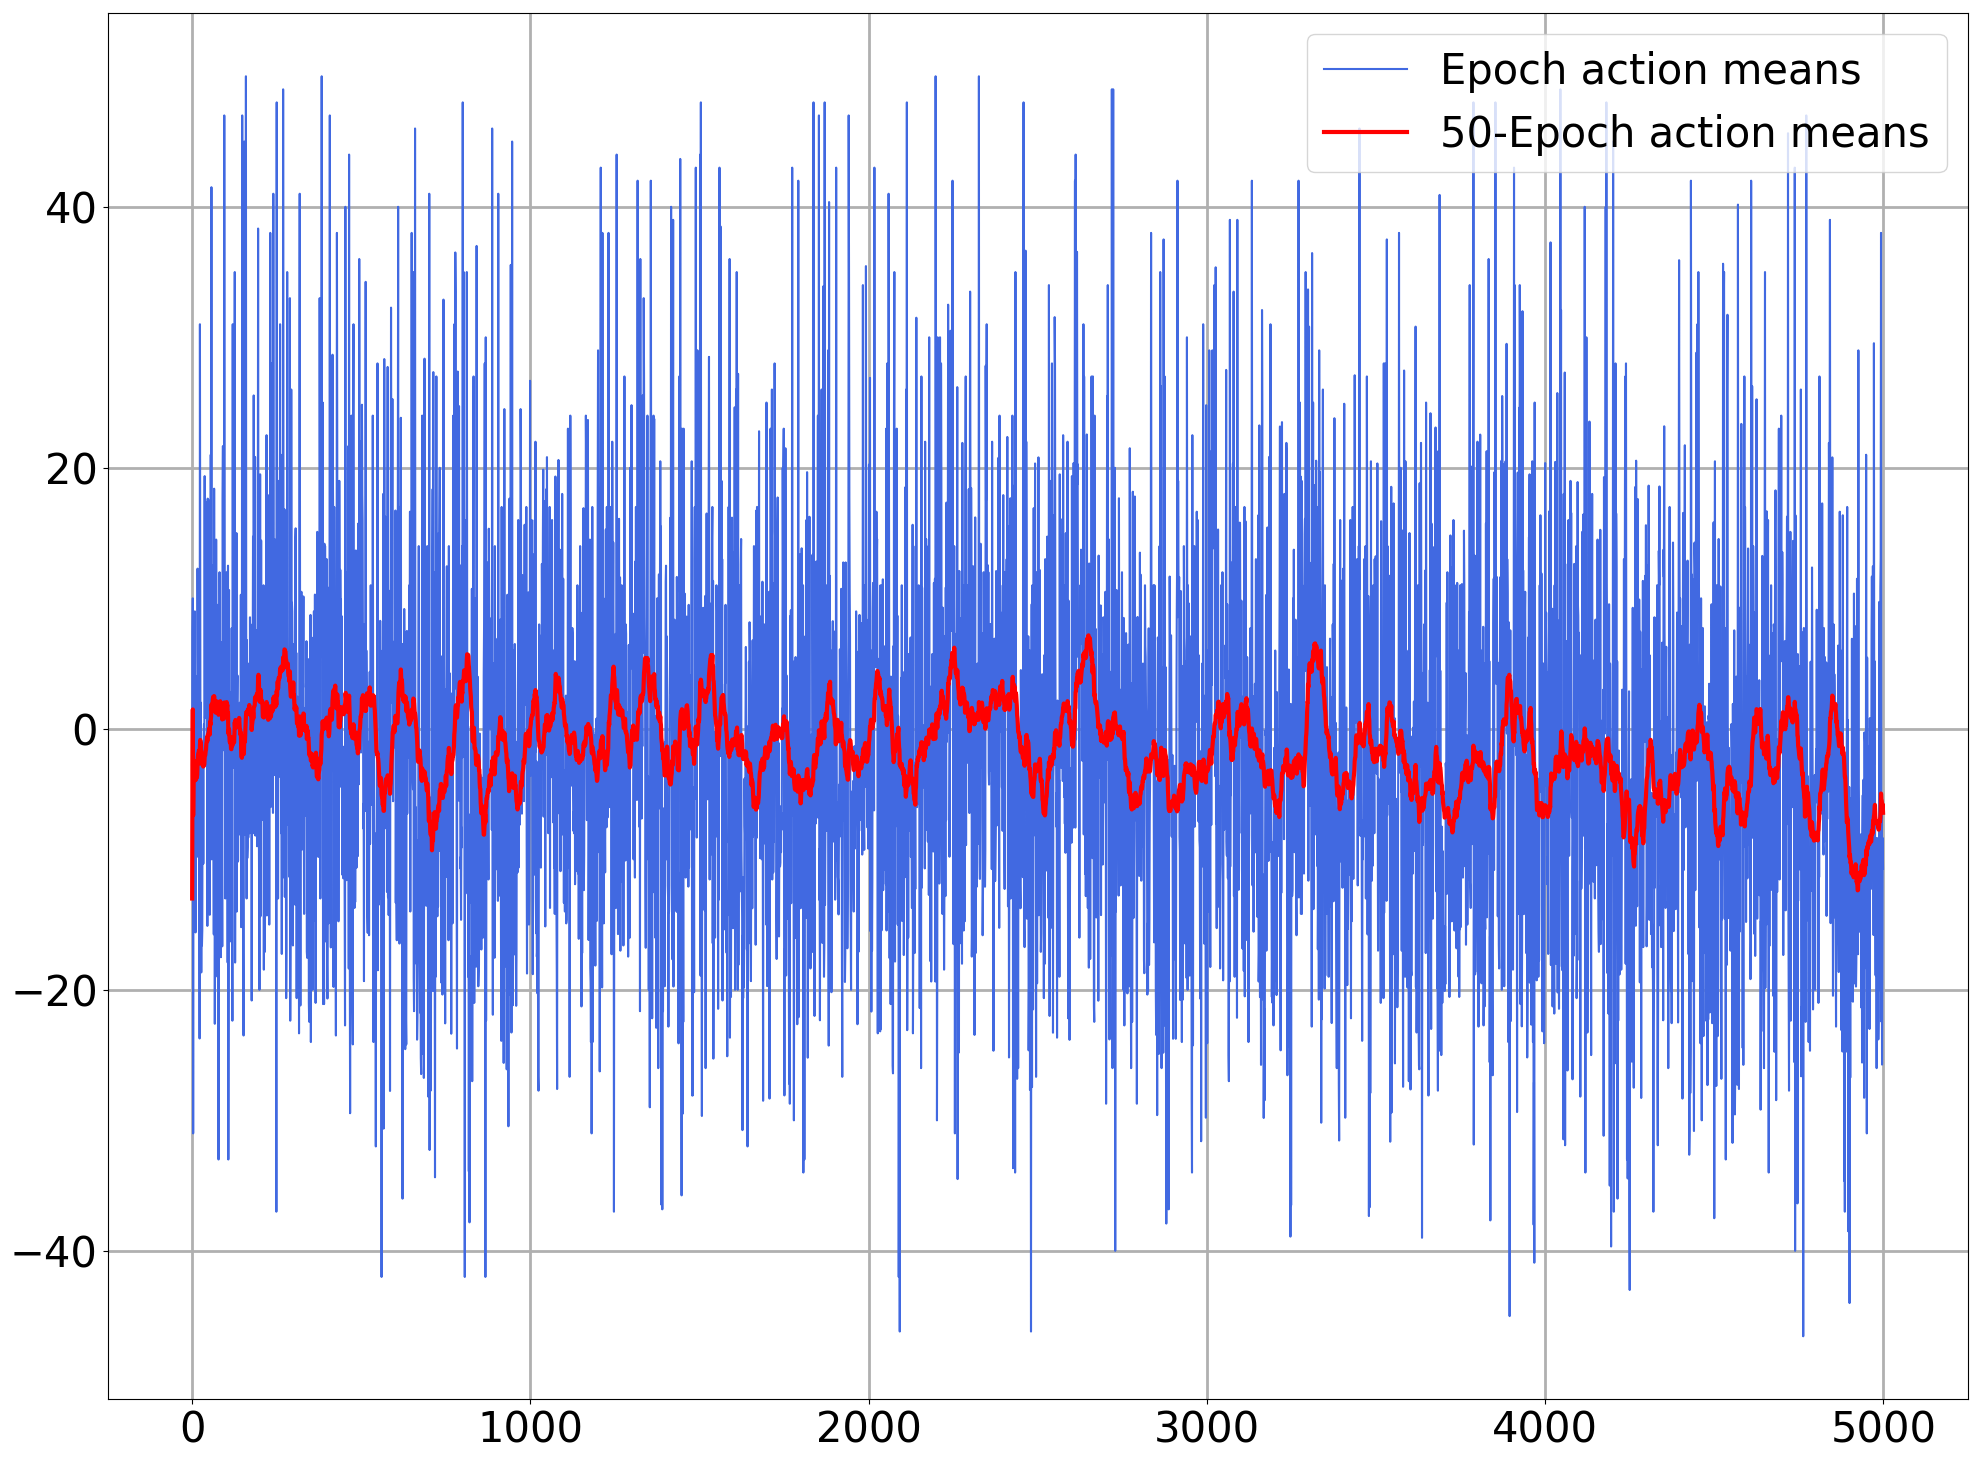
\includegraphics[width=\textwidth]{cnn_1_sell_mean_actions.png}
        \caption{Mean of actions per epoch (sell)}
        \label{fig:analysis-dqn-1-action-sell}
    \end{subfigure}
    \caption{DQN agent rewards and mean of actions for buying and selling on training data set I using feature I.}
    \label{fig:analysis-dqn-1}
\end{figure}

\begin{figure}[H]
    \centering
    \begin{subfigure}[b]{0.45\textwidth}
        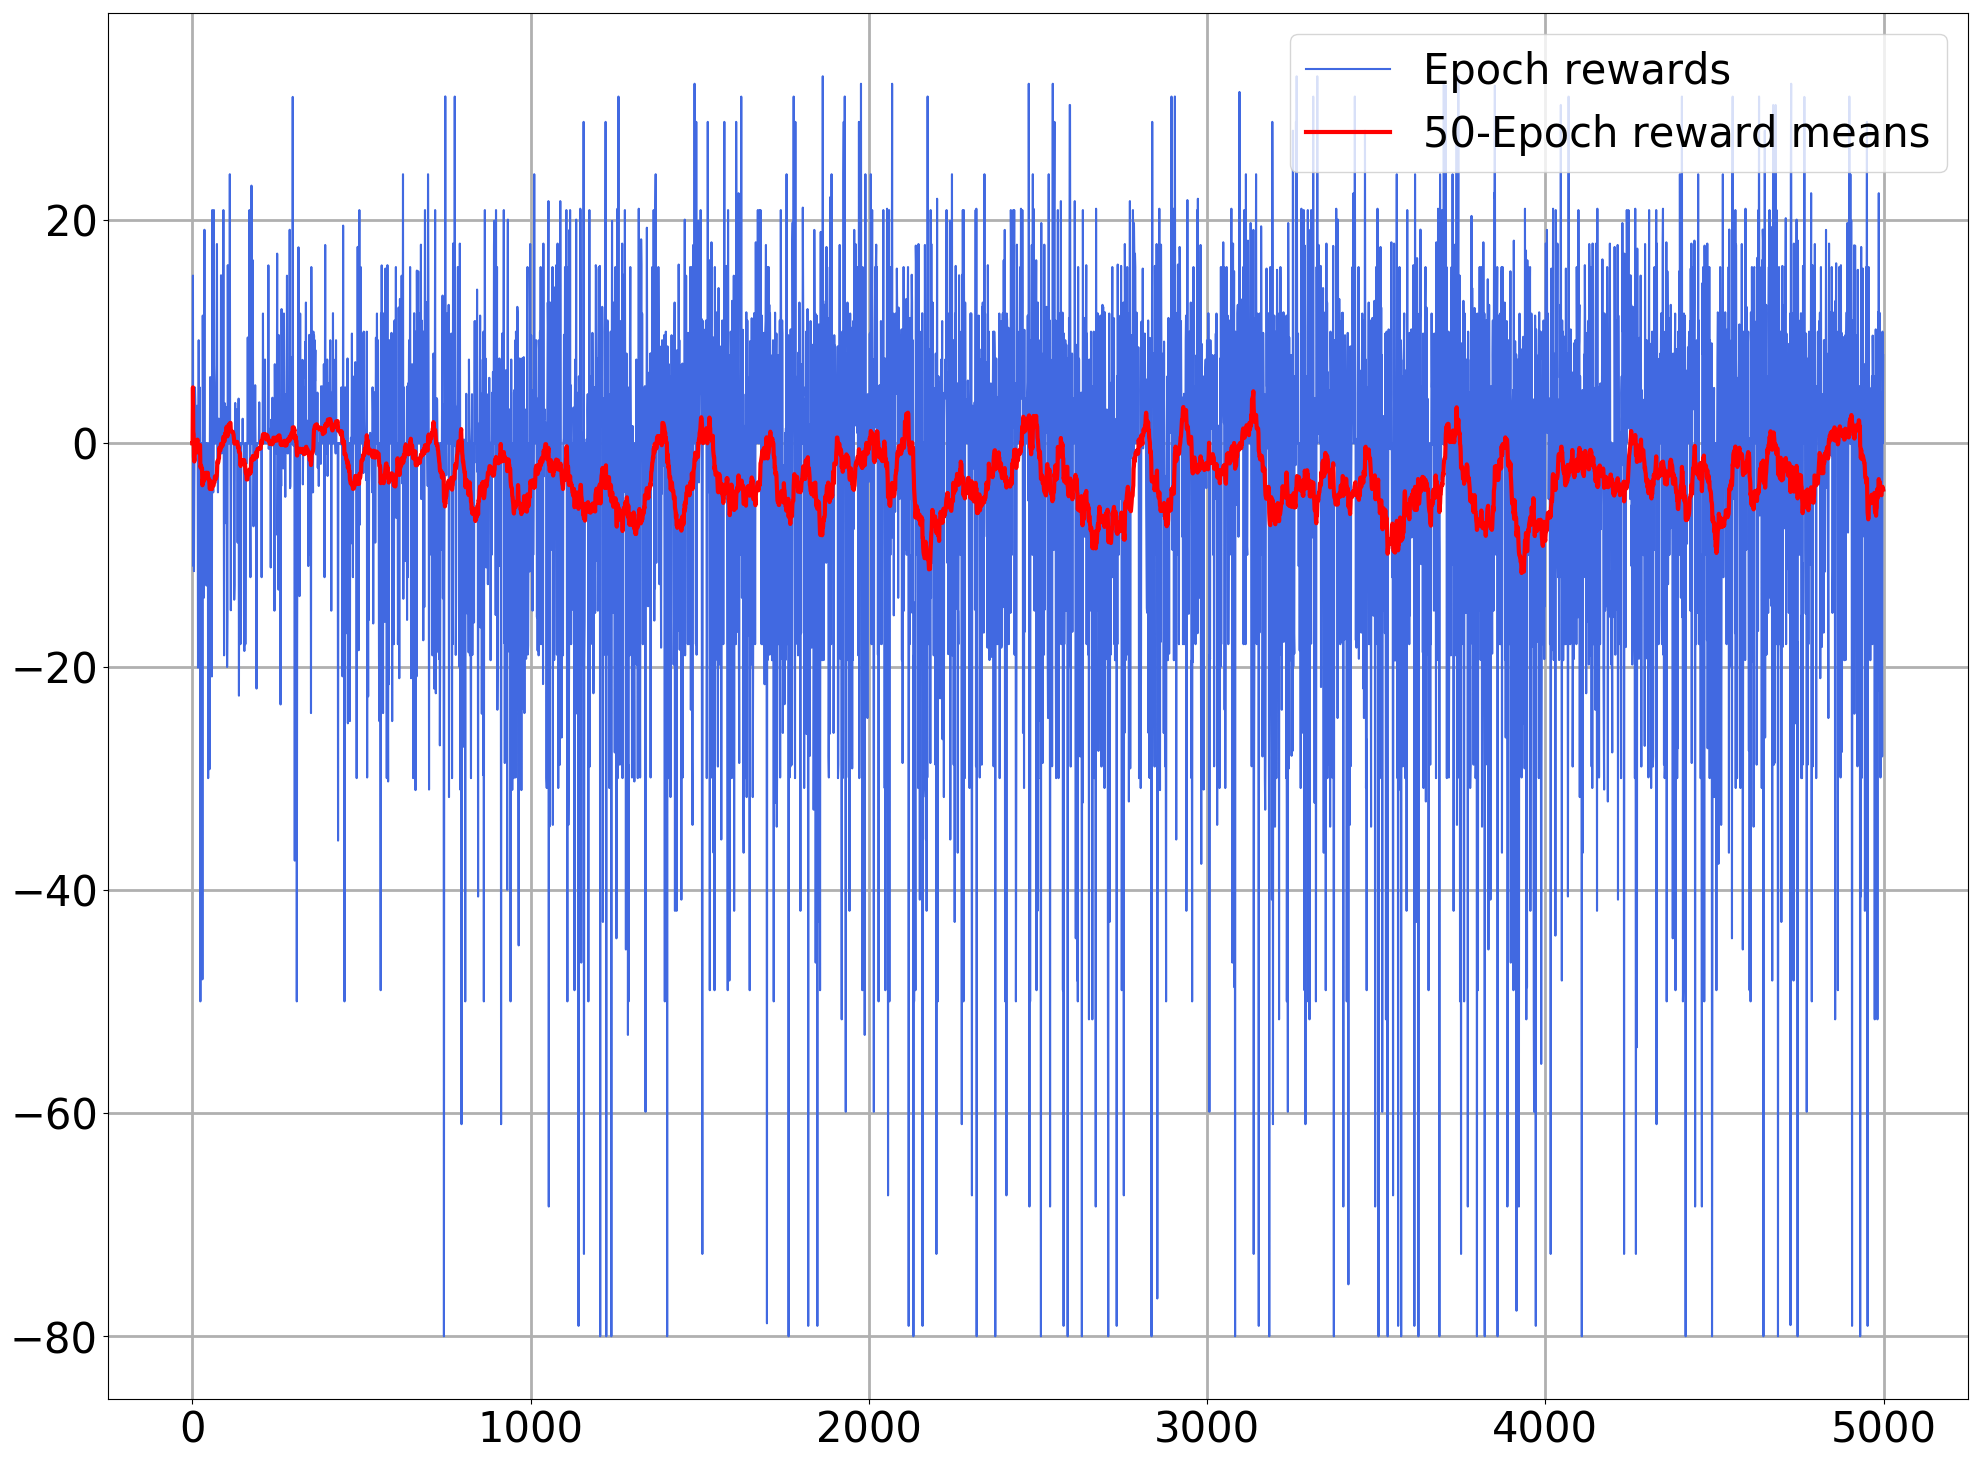
\includegraphics[width=\textwidth]{cnn_2_buy_rewards.png}
        \caption{Reward per epoch (buy)}
        \label{fig:analysis-dqn-1-reward-buy}
    \end{subfigure}
    \begin{subfigure}[b]{0.45\textwidth}
        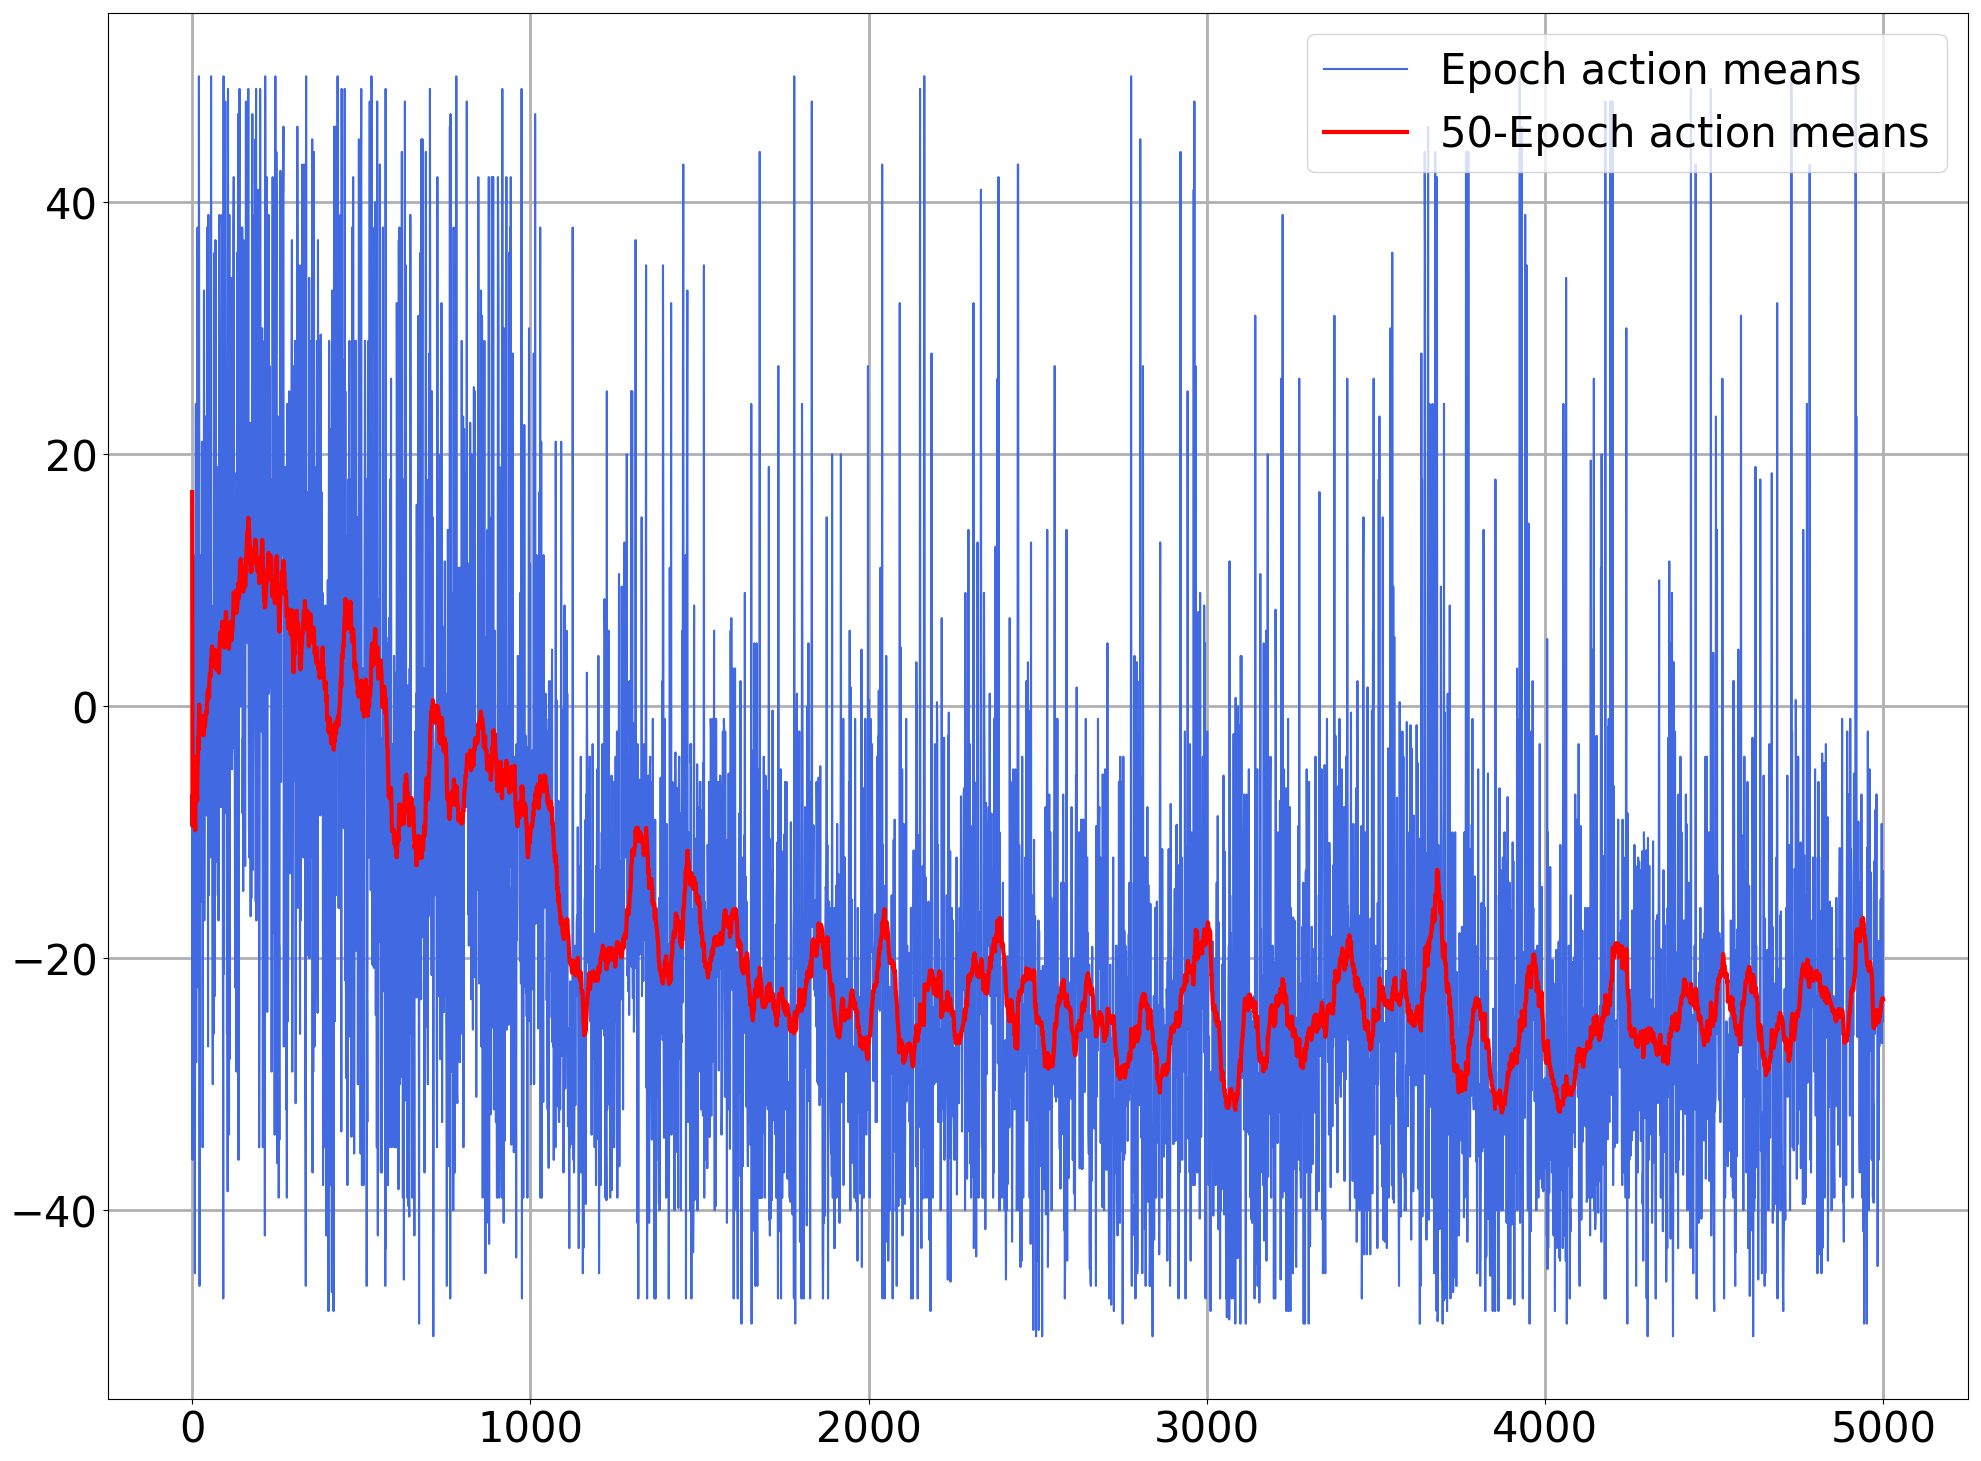
\includegraphics[width=\textwidth]{cnn_2_buy_mean_actions.png}
        \caption{Mean of actions per epoch (buy)}
        \label{fig:analysis-dqn-1-action-buy}
    \end{subfigure}
    \begin{subfigure}[b]{0.45\textwidth}
        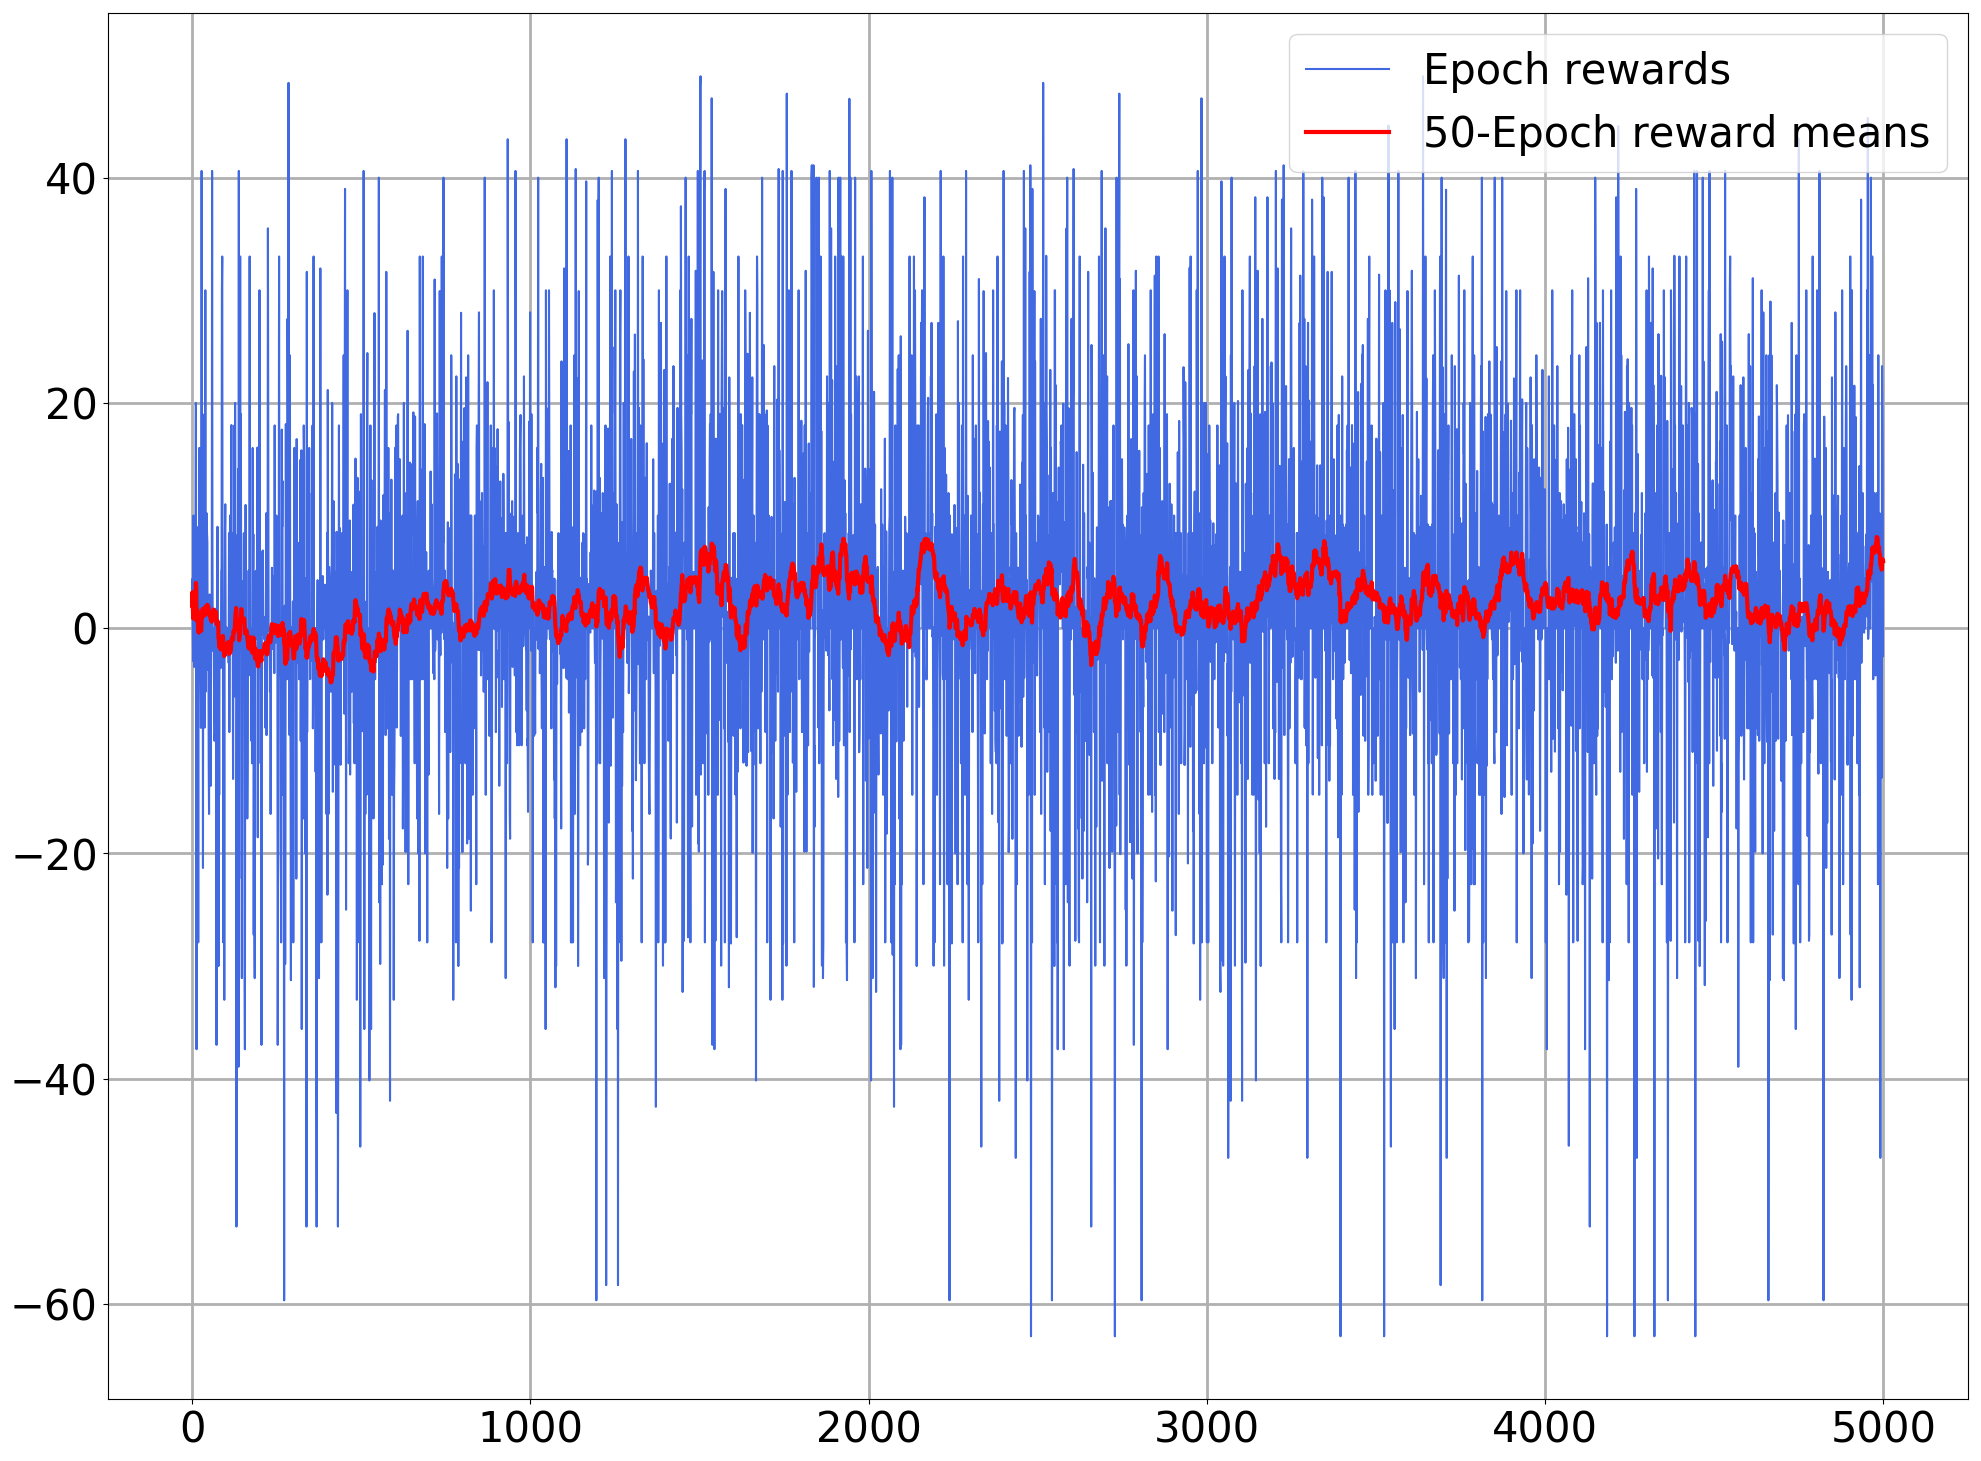
\includegraphics[width=\textwidth]{cnn_2_sell_rewards.png}
        \caption{Mean rewards per epoch (sell)}
        \label{fig:analysis-dqn-1-reward-sell}
    \end{subfigure}
    \begin{subfigure}[b]{0.45\textwidth}
        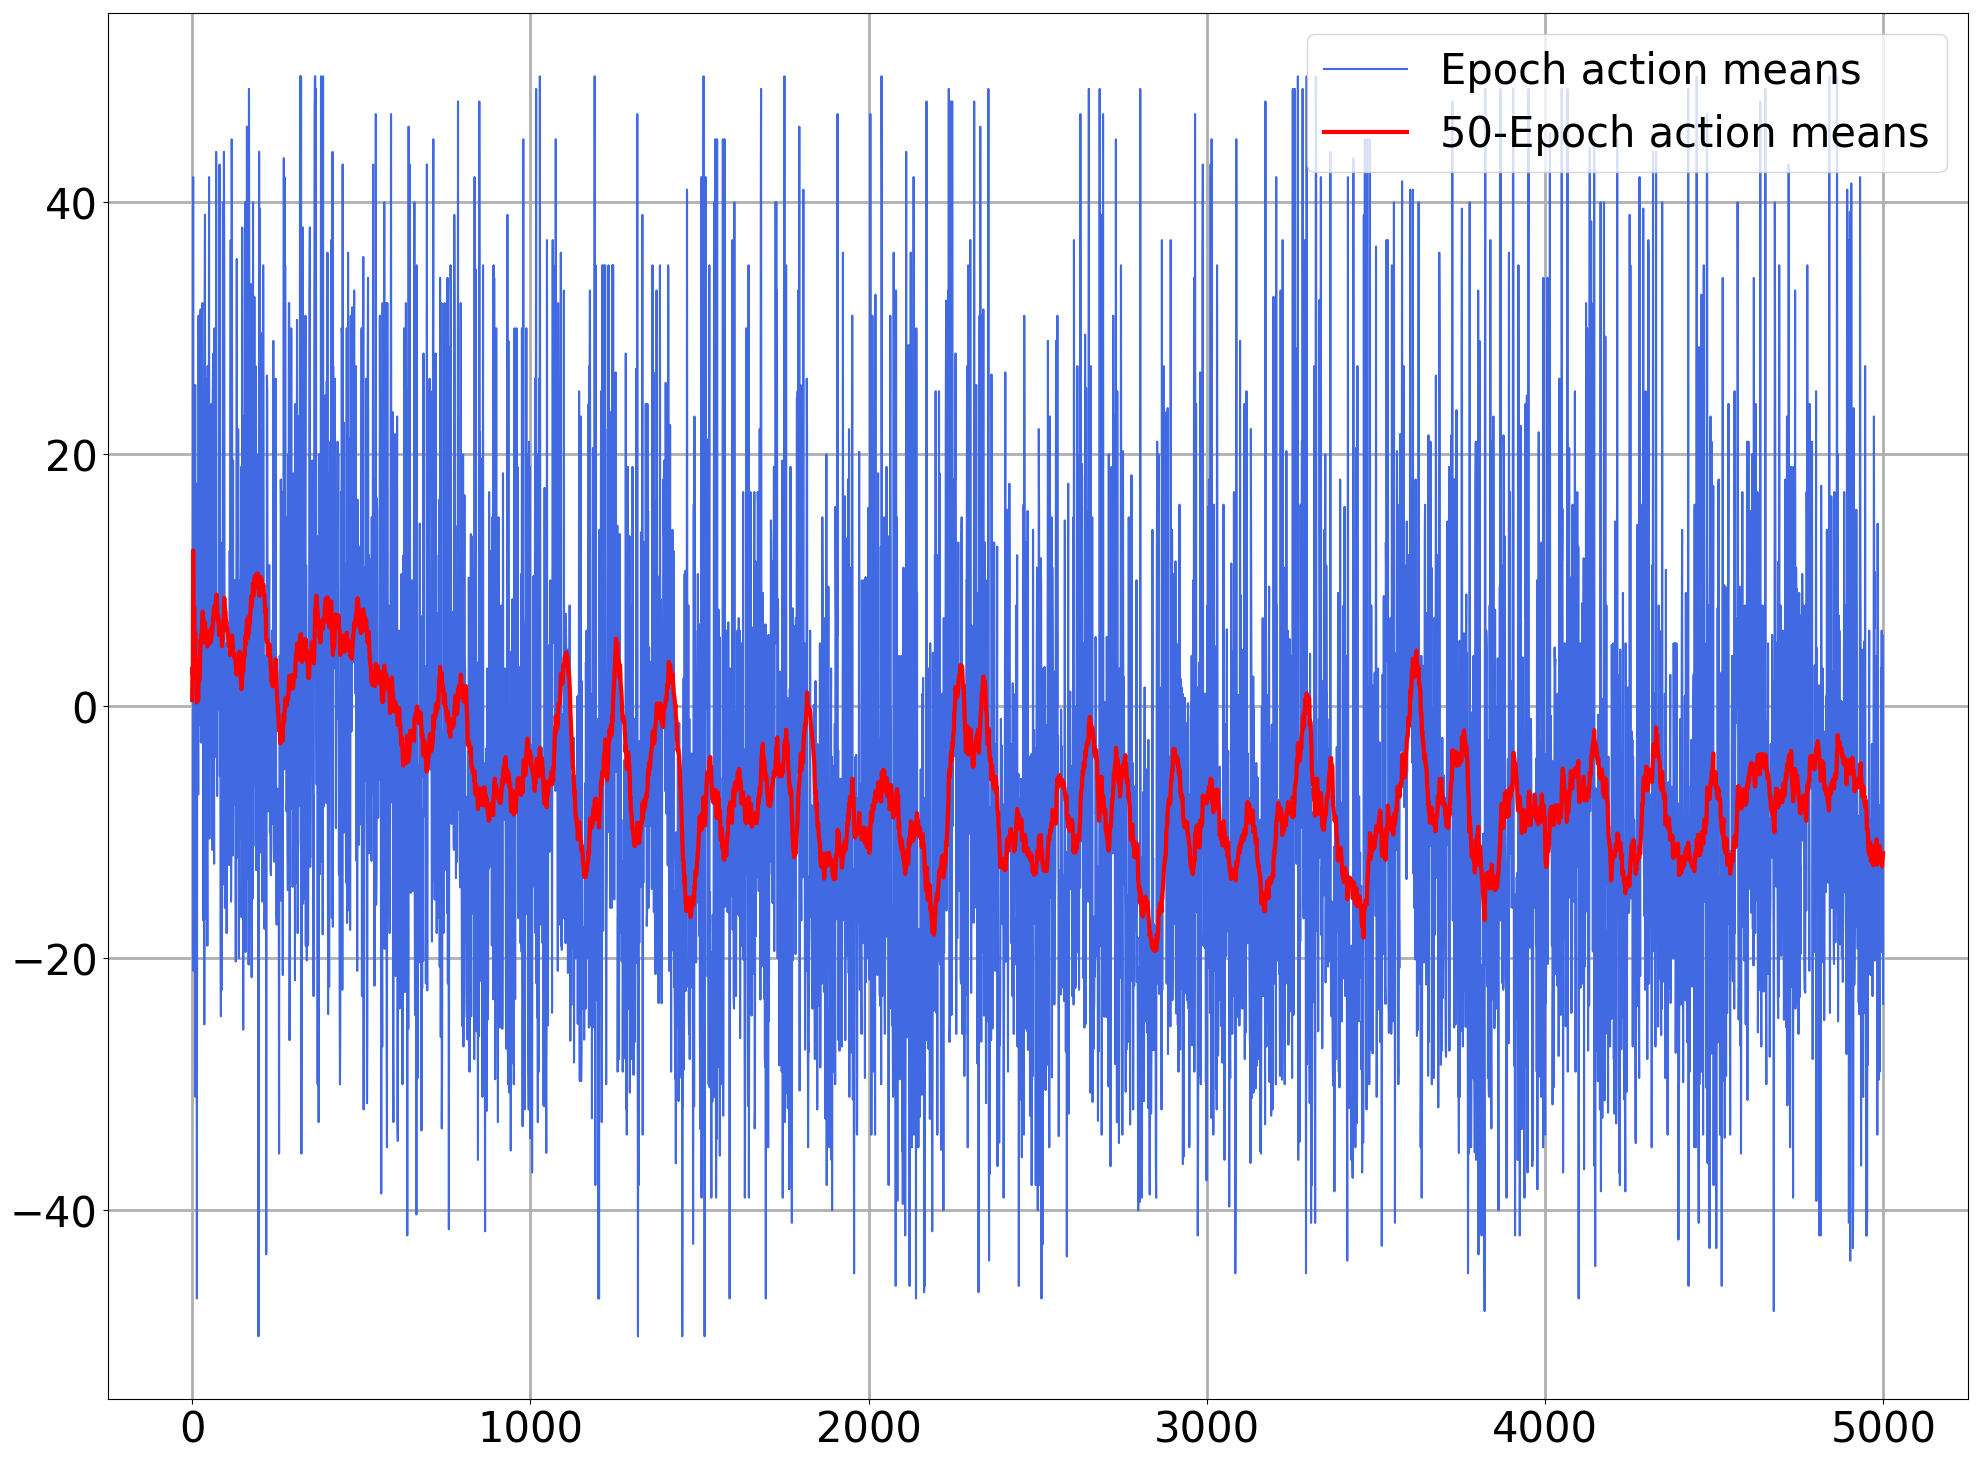
\includegraphics[width=\textwidth]{cnn_2_sell_mean_actions.png}
        \caption{Mean of actions per epoch (sell)}
        \label{fig:analysis-dqn-1-action-sell}
    \end{subfigure}
    \caption{DQN agent rewards and mean of actions for buying and selling on training data set II using feature I.}
    \label{fig:analysis-dqn-2}
\end{figure}


\begin{table}[H]
\centering
\begin{tabular}{l|l|l|}
\cline{2-3}
& \textbf{DQN (Feature I)} & \textbf{\begin{tabular}[c]{@{}l@{}}Market\\ Order\end{tabular}} \\ \hline
\multicolumn{1}{|l|}{\textbf{Buy (I)}}   & 22.06          & -0.05                                                           \\ \hline
\multicolumn{1}{|l|}{\textbf{Sell (I)}}  & -49.26         & -27.70                                                          \\ \hline
\multicolumn{1}{|l|}{\textbf{Buy (II)}}  & -2.26          & -1.06                                                           \\ \hline
\multicolumn{1}{|l|}{\textbf{Sell (II)}} & 0.84          & -1.72                                                           \\ \hline
\end{tabular}
\caption{Summary of rewards for the Q-Learning agent and market orders.}
\label{tbl:analysis-dqn-orderfeature-summary}
\end{table}

\subsection{Application of historical trade feature}

\begin{figure}[H]
    \centering
    \begin{subfigure}[b]{0.45\textwidth}
        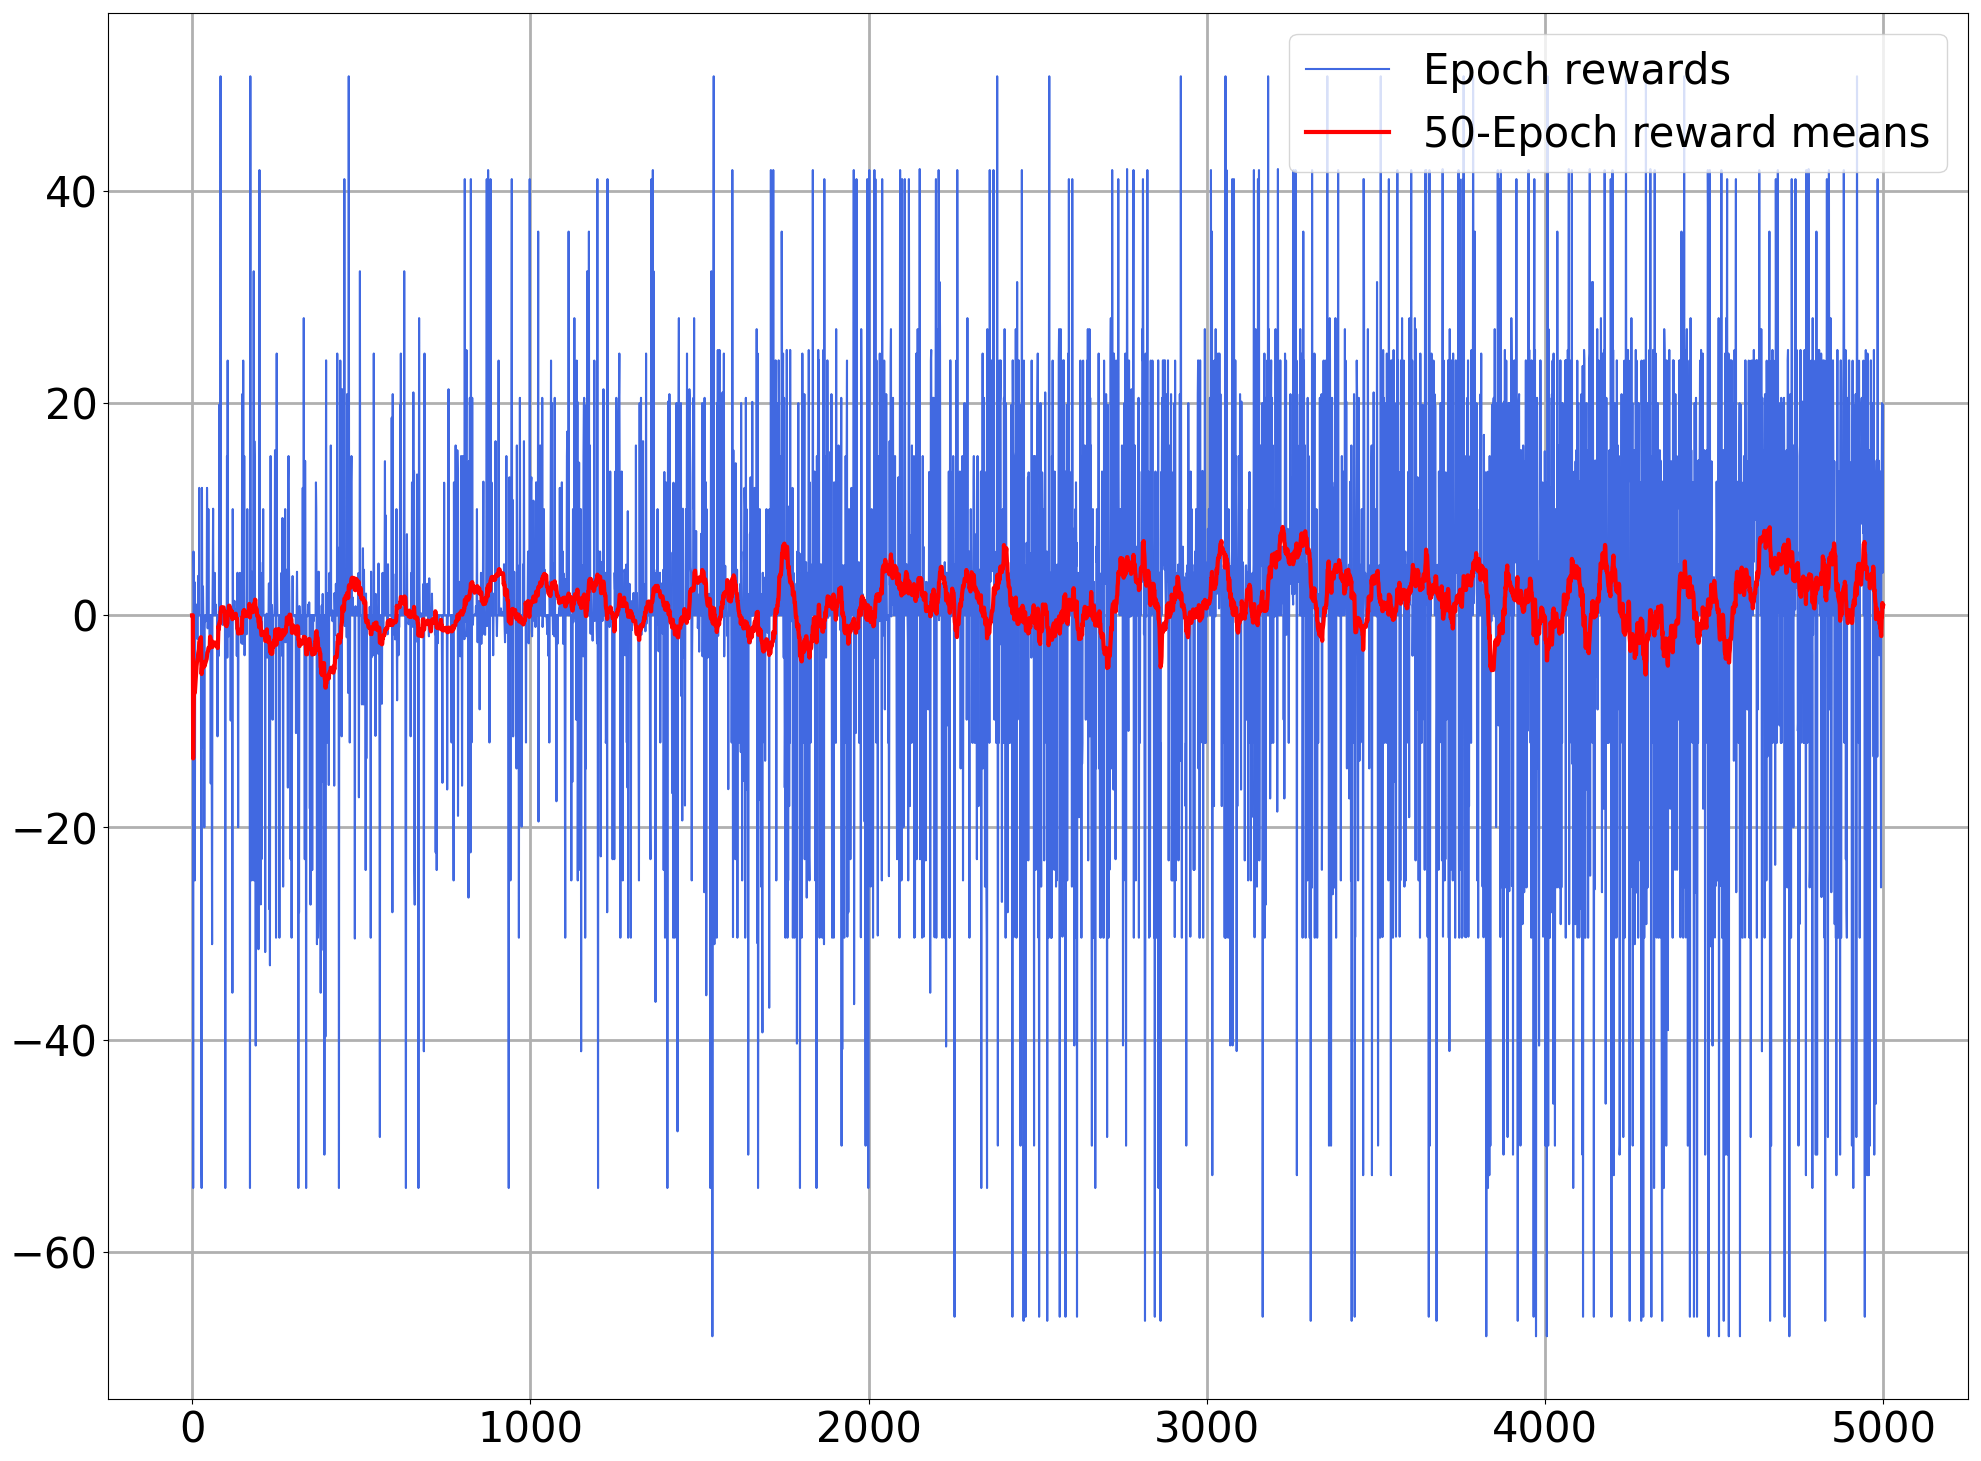
\includegraphics[width=\textwidth]{cnn_1_buy_trades_rewards.png}
        \caption{Reward per epoch (buy)}
        \label{fig:analysis-dqn-1-trades-reward-buy}
    \end{subfigure}
    \begin{subfigure}[b]{0.45\textwidth}
        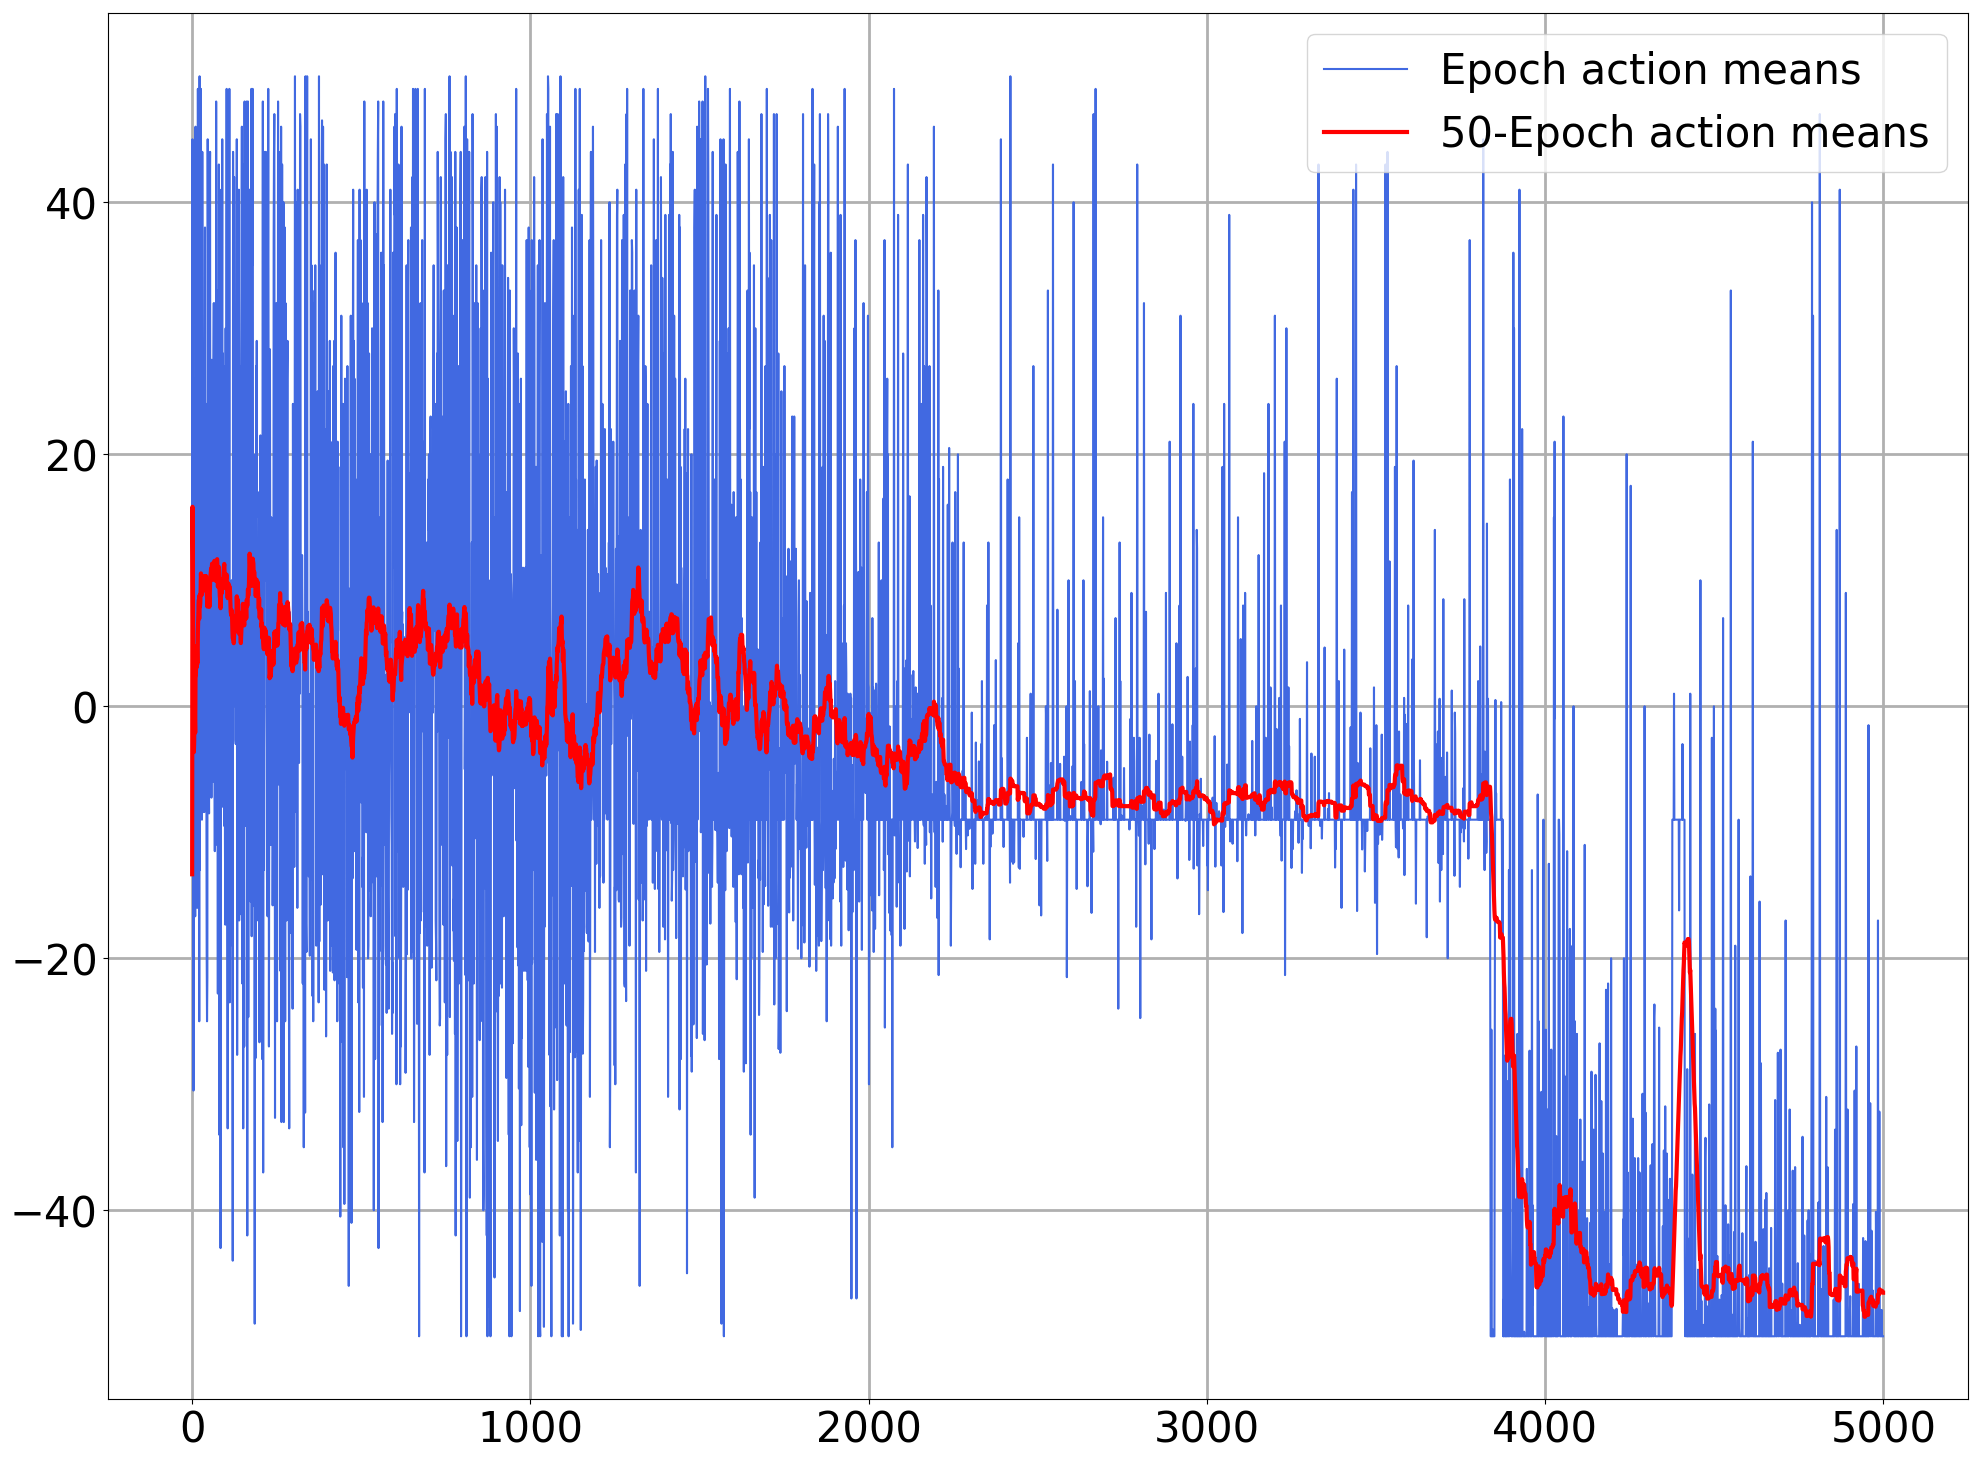
\includegraphics[width=\textwidth]{cnn_1_buy_trades_mean_actions.png}
        \caption{Mean of actions per epoch (buy)}
        \label{fig:analysis-dqn-1-trades-action-buy}
    \end{subfigure}
    \begin{subfigure}[b]{0.45\textwidth}
        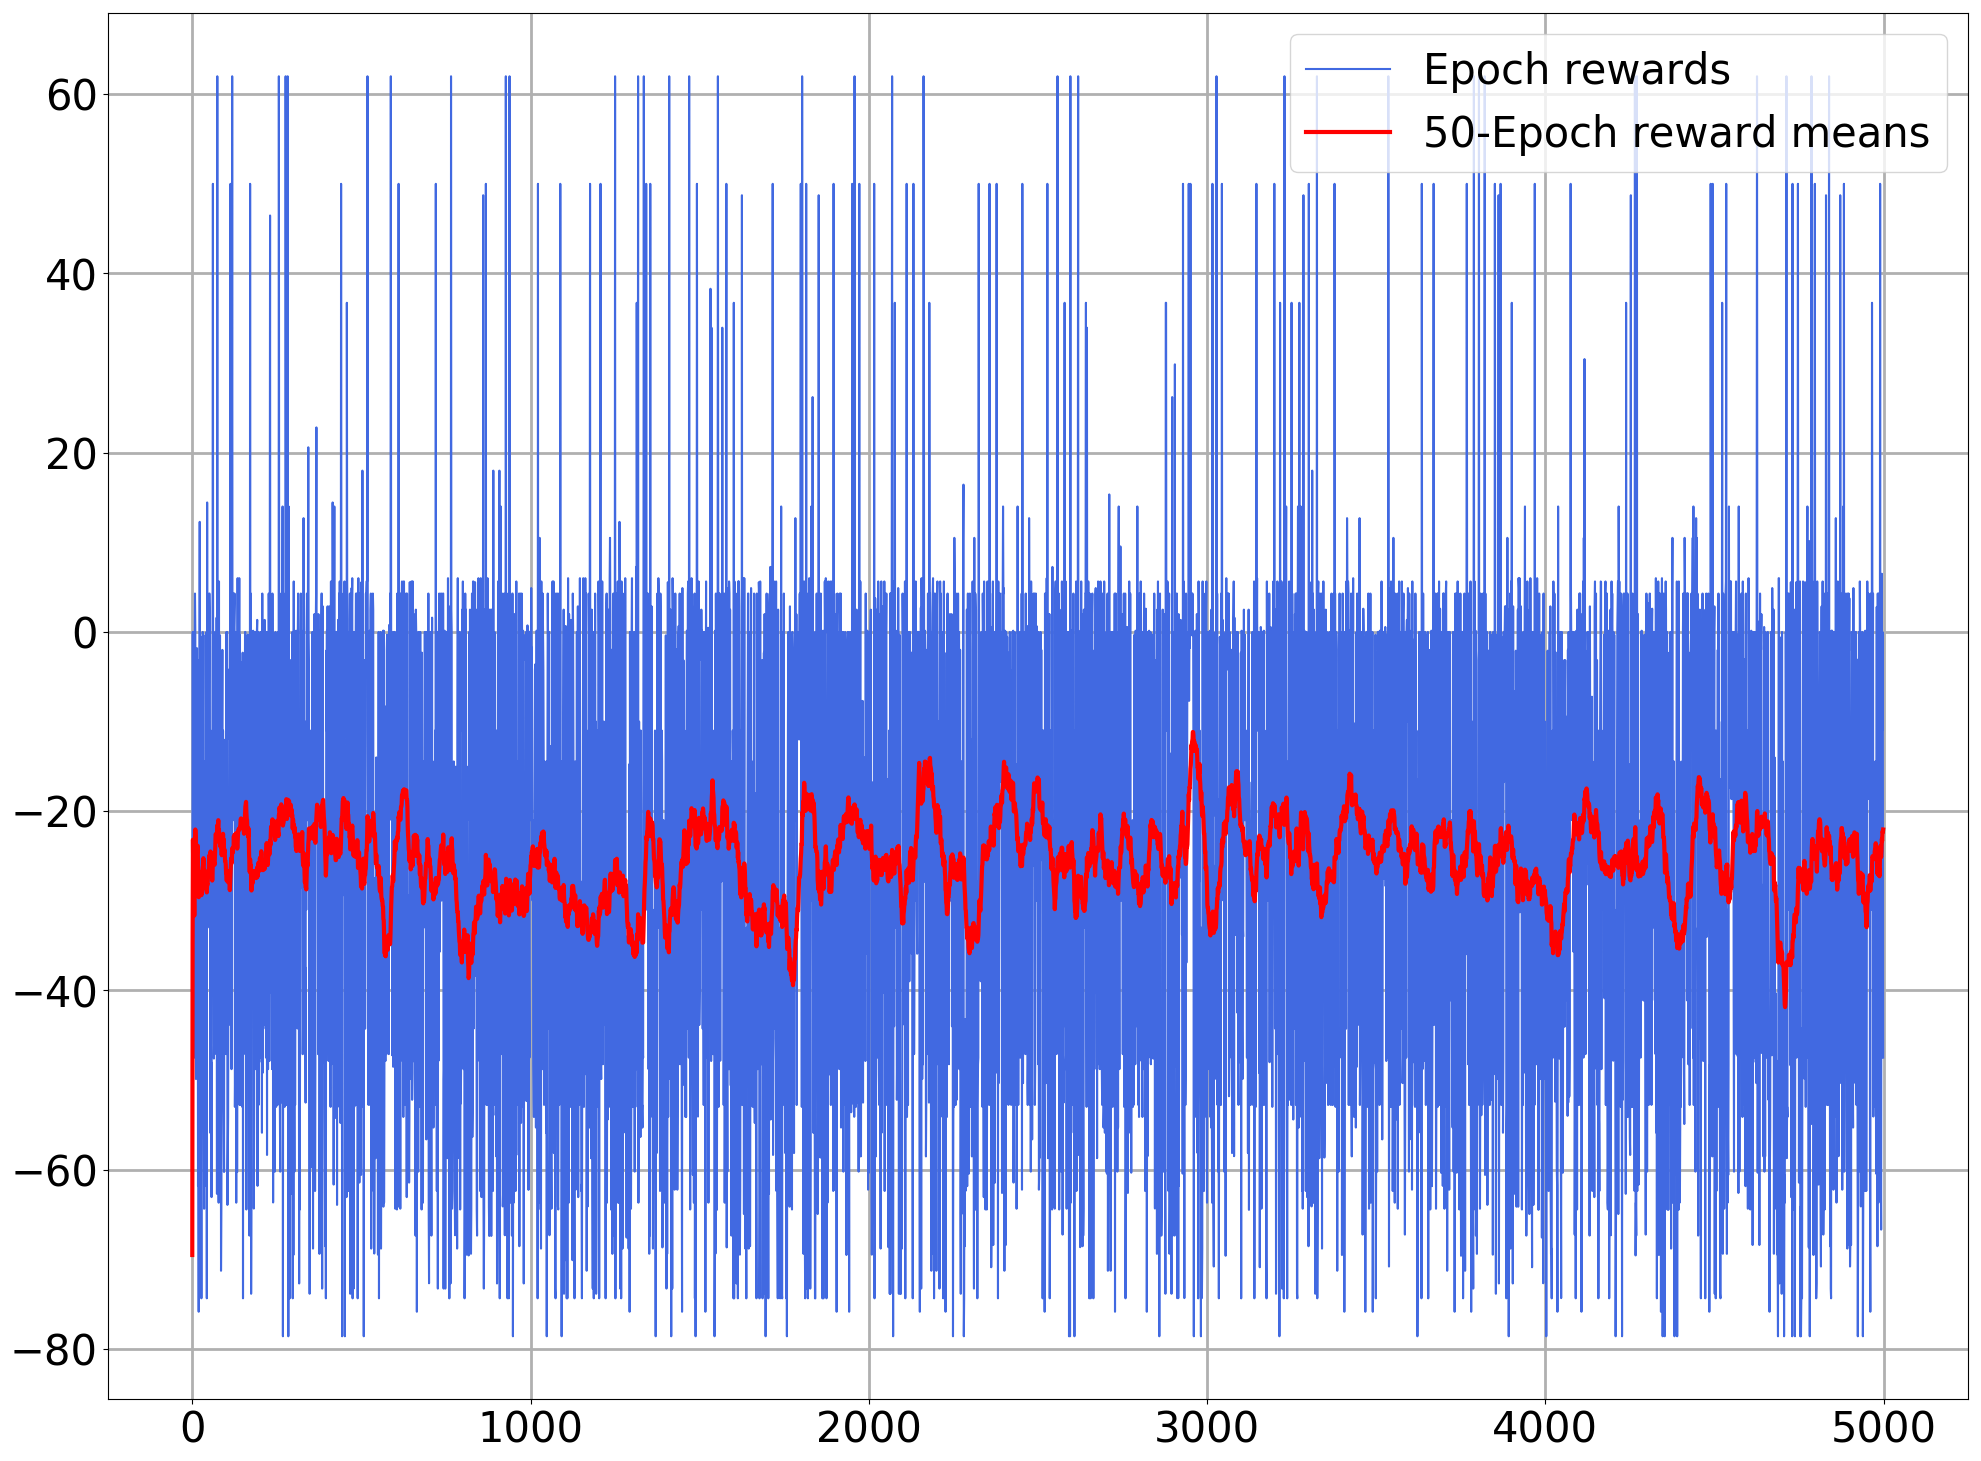
\includegraphics[width=\textwidth]{cnn_1_sell_trades_rewards.png}
        \caption{Mean rewards per epoch (sell)}
        \label{fig:analysis-dqn-1-trades-reward-sell}
    \end{subfigure}
    \begin{subfigure}[b]{0.45\textwidth}
        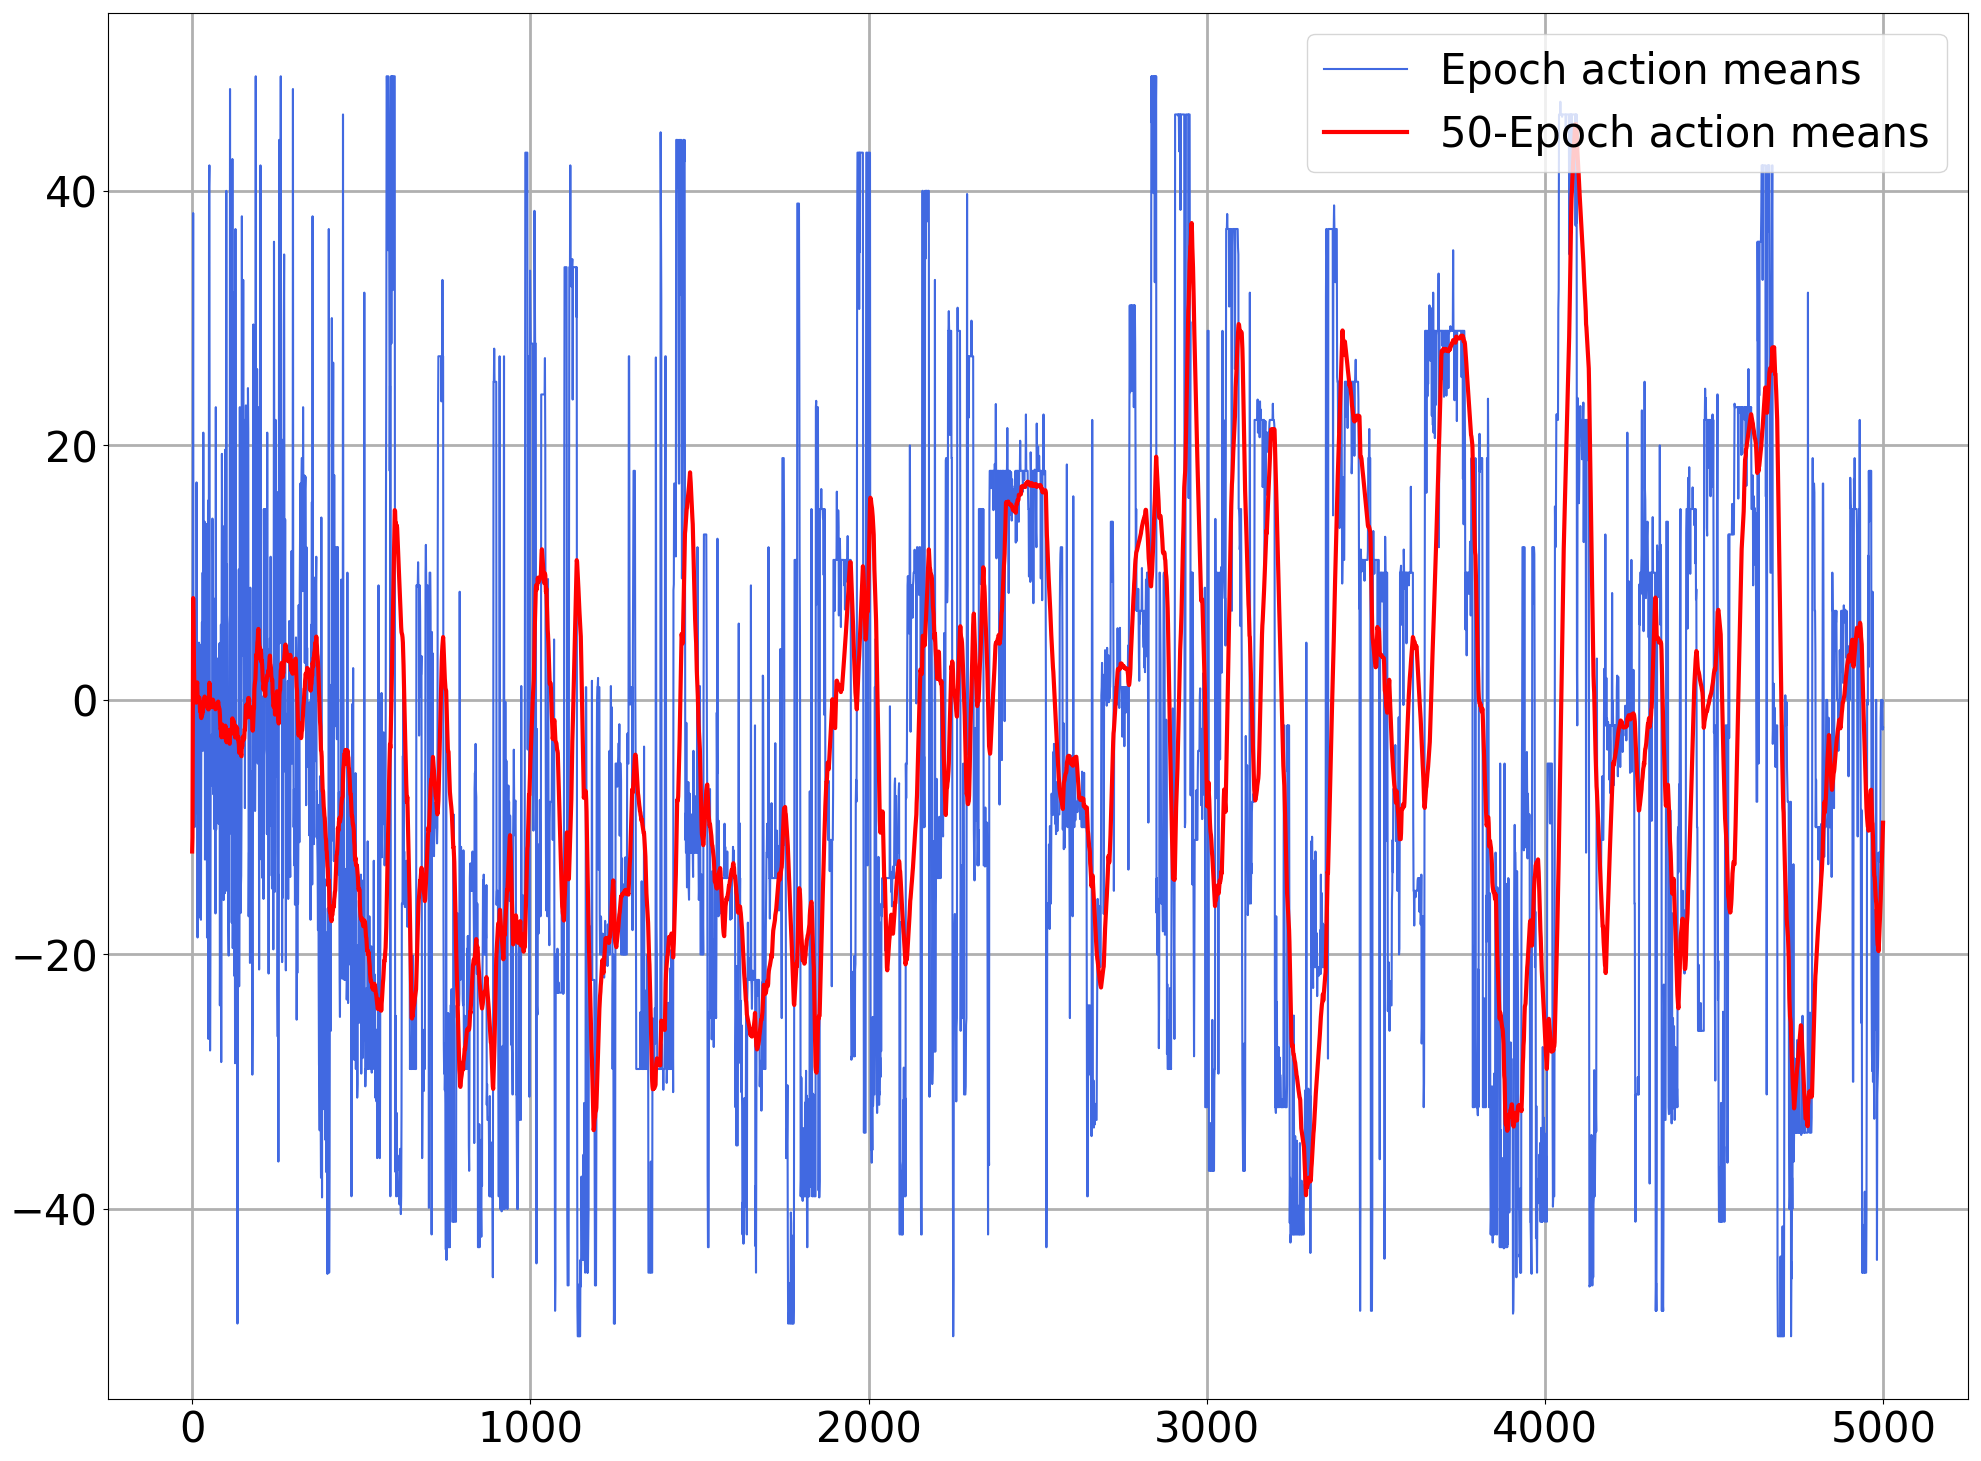
\includegraphics[width=\textwidth]{cnn_1_sell_trades_mean_actions.png}
        \caption{Mean of actions per epoch (sell)}
        \label{fig:analysis-dqn-1-trades-action-sell}
    \end{subfigure}
    \caption{DQN agent rewards and mean of actions for buying and selling on training data set I using feature II.}
    \label{fig:analysis-dqn-1}
\end{figure}

\begin{figure}[H]
    \centering
    \begin{subfigure}[b]{0.45\textwidth}
        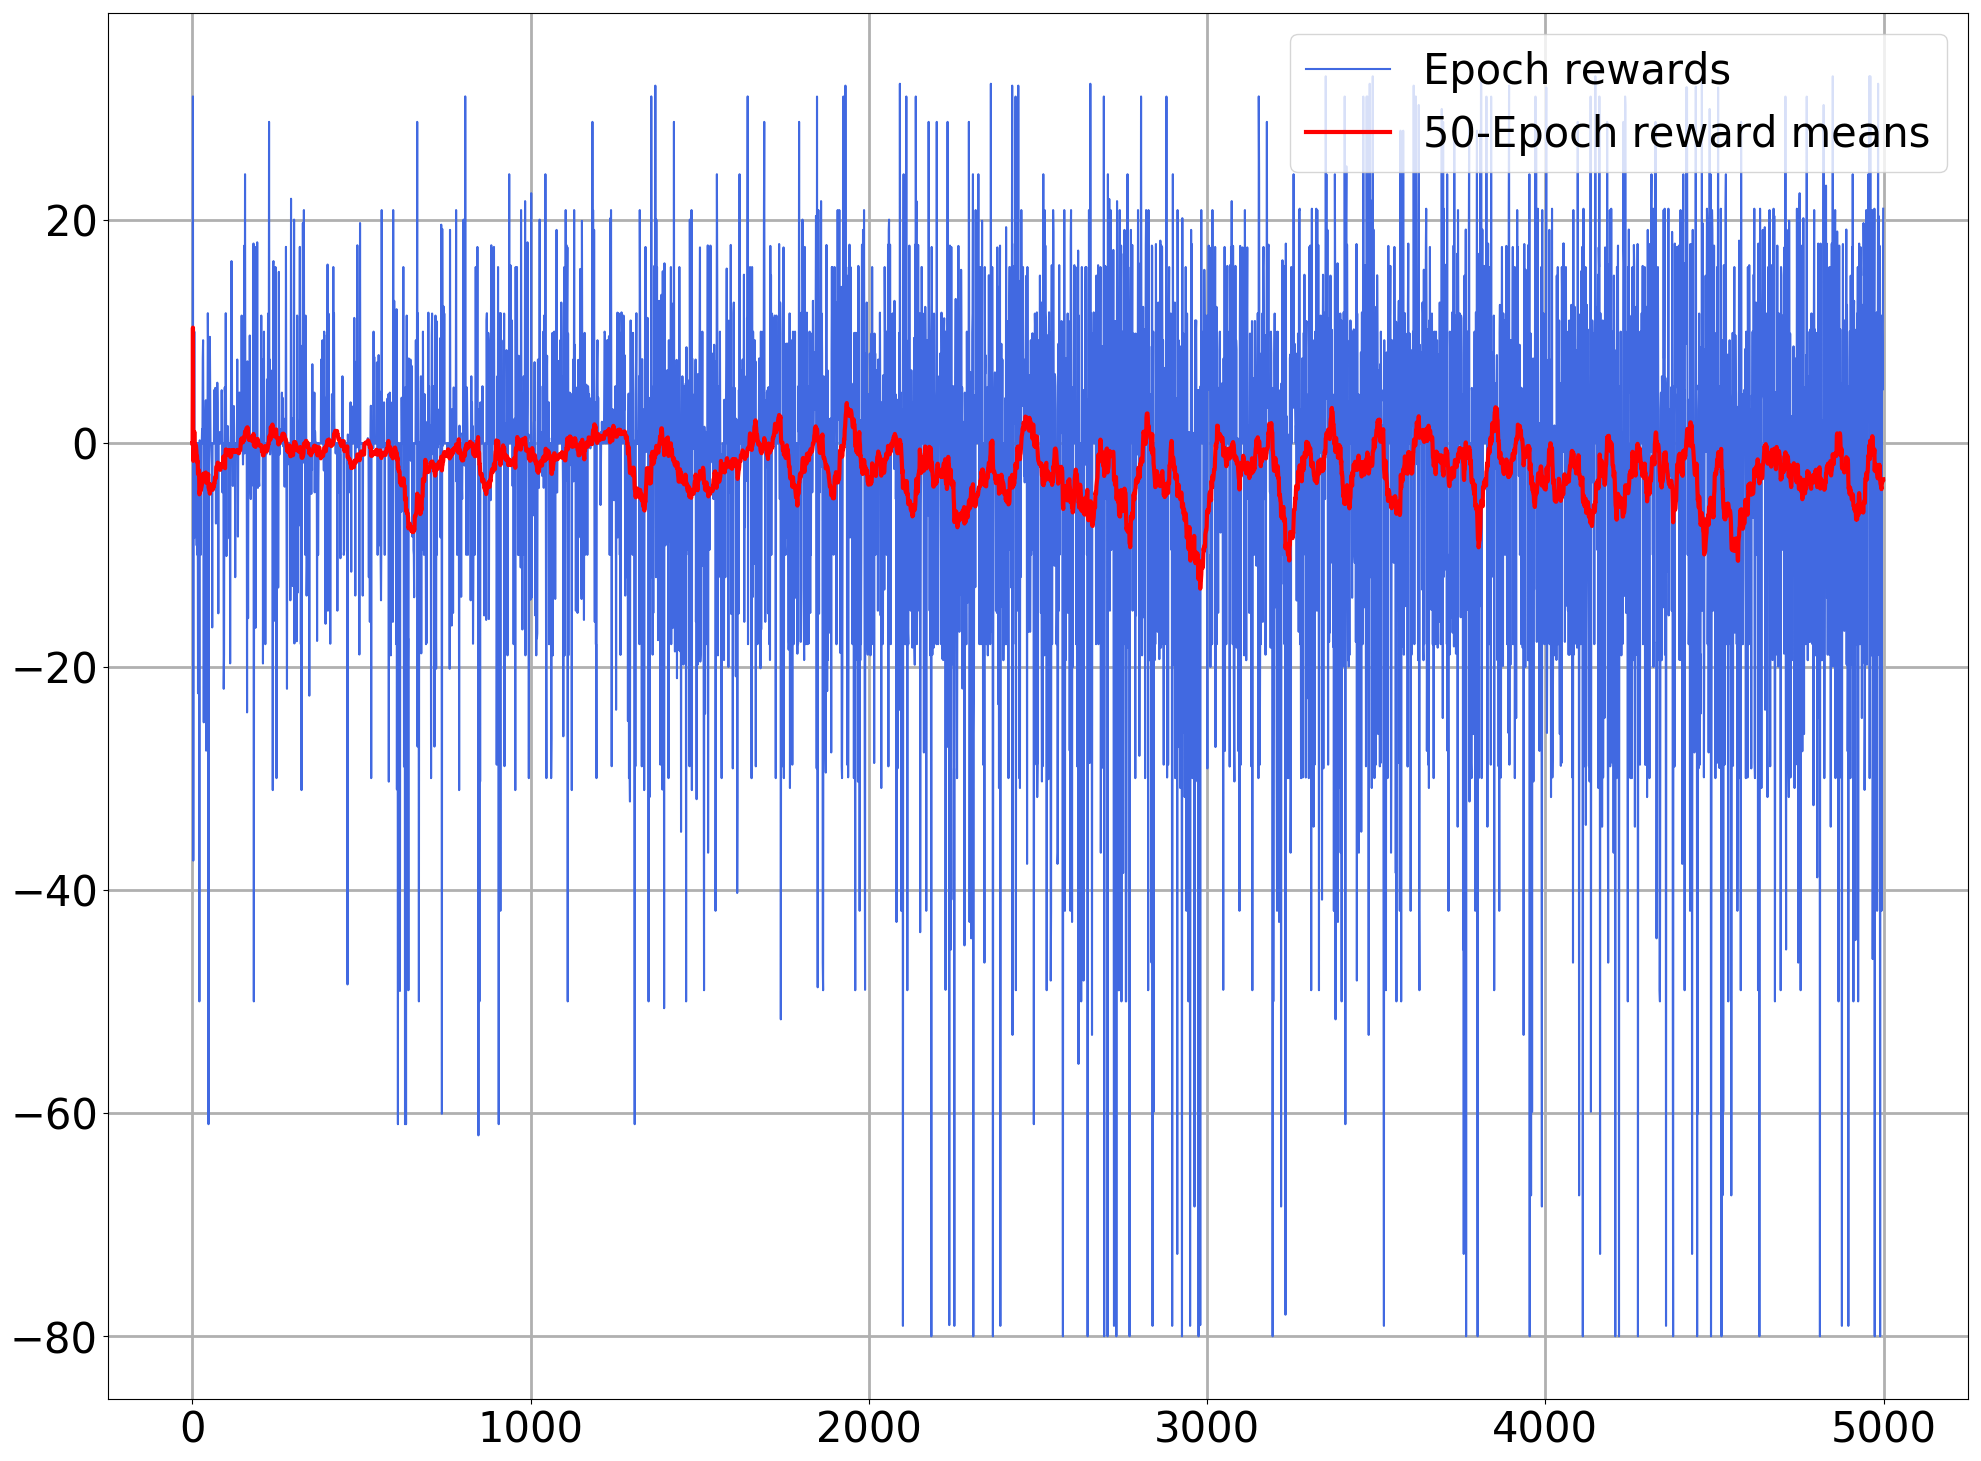
\includegraphics[width=\textwidth]{cnn_2_buy_trades_rewards.png}
        \caption{Reward per epoch (buy)}
        \label{fig:analysis-dqn-1-trades-reward-buy}
    \end{subfigure}
    \begin{subfigure}[b]{0.45\textwidth}
        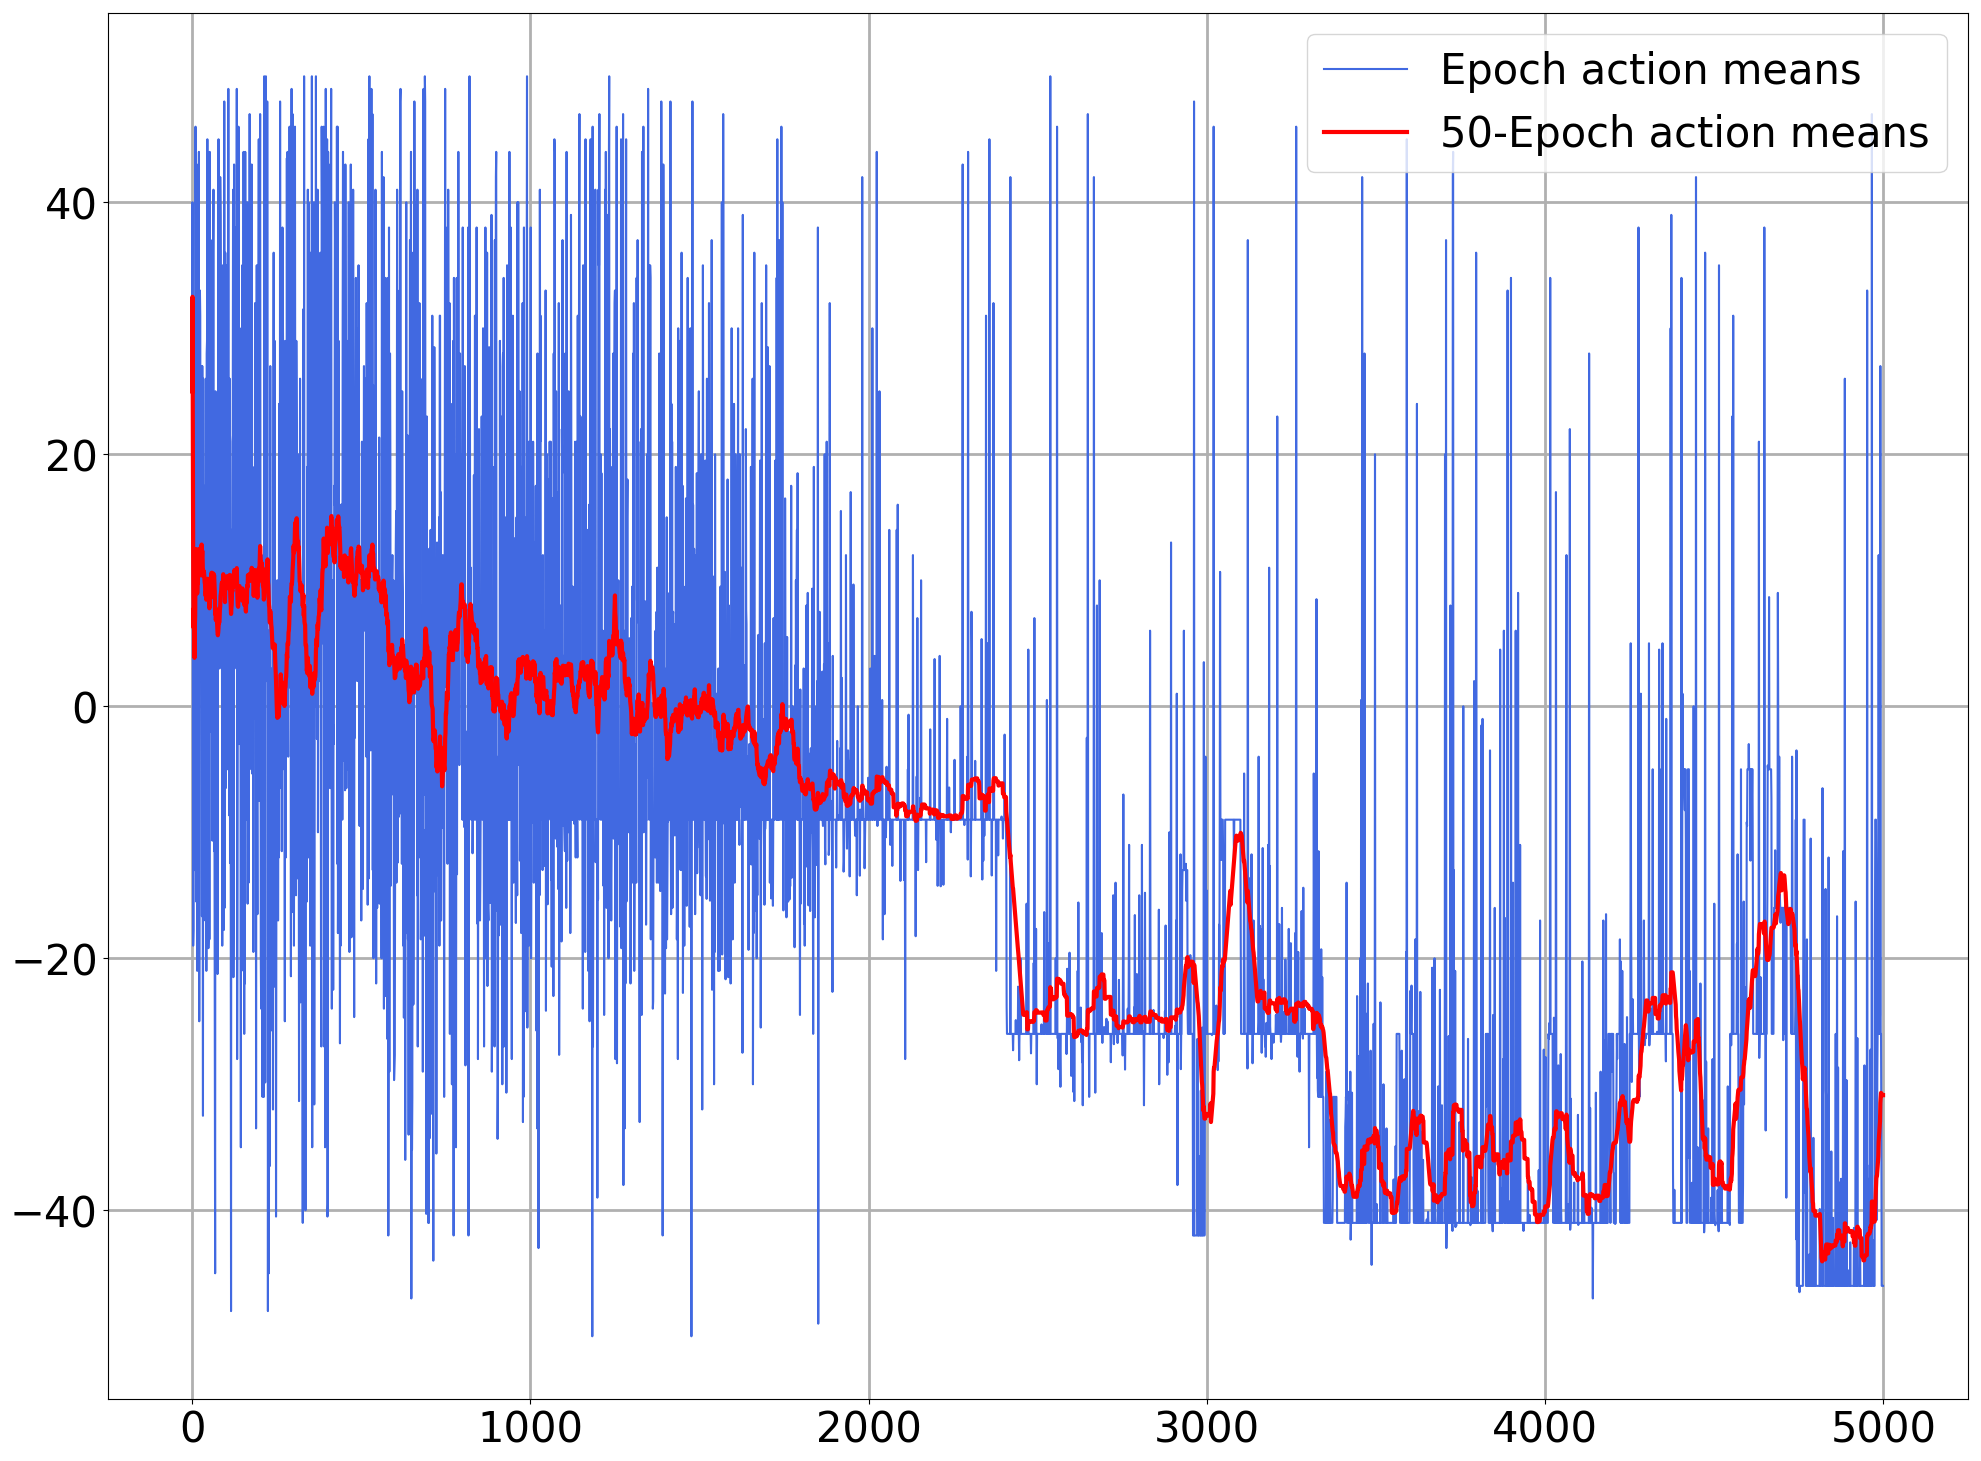
\includegraphics[width=\textwidth]{cnn_2_buy_trades_mean_actions.png}
        \caption{Mean of actions per epoch (buy)}
        \label{fig:analysis-dqn-1-trades-action-buy}
    \end{subfigure}
    \begin{subfigure}[b]{0.45\textwidth}
        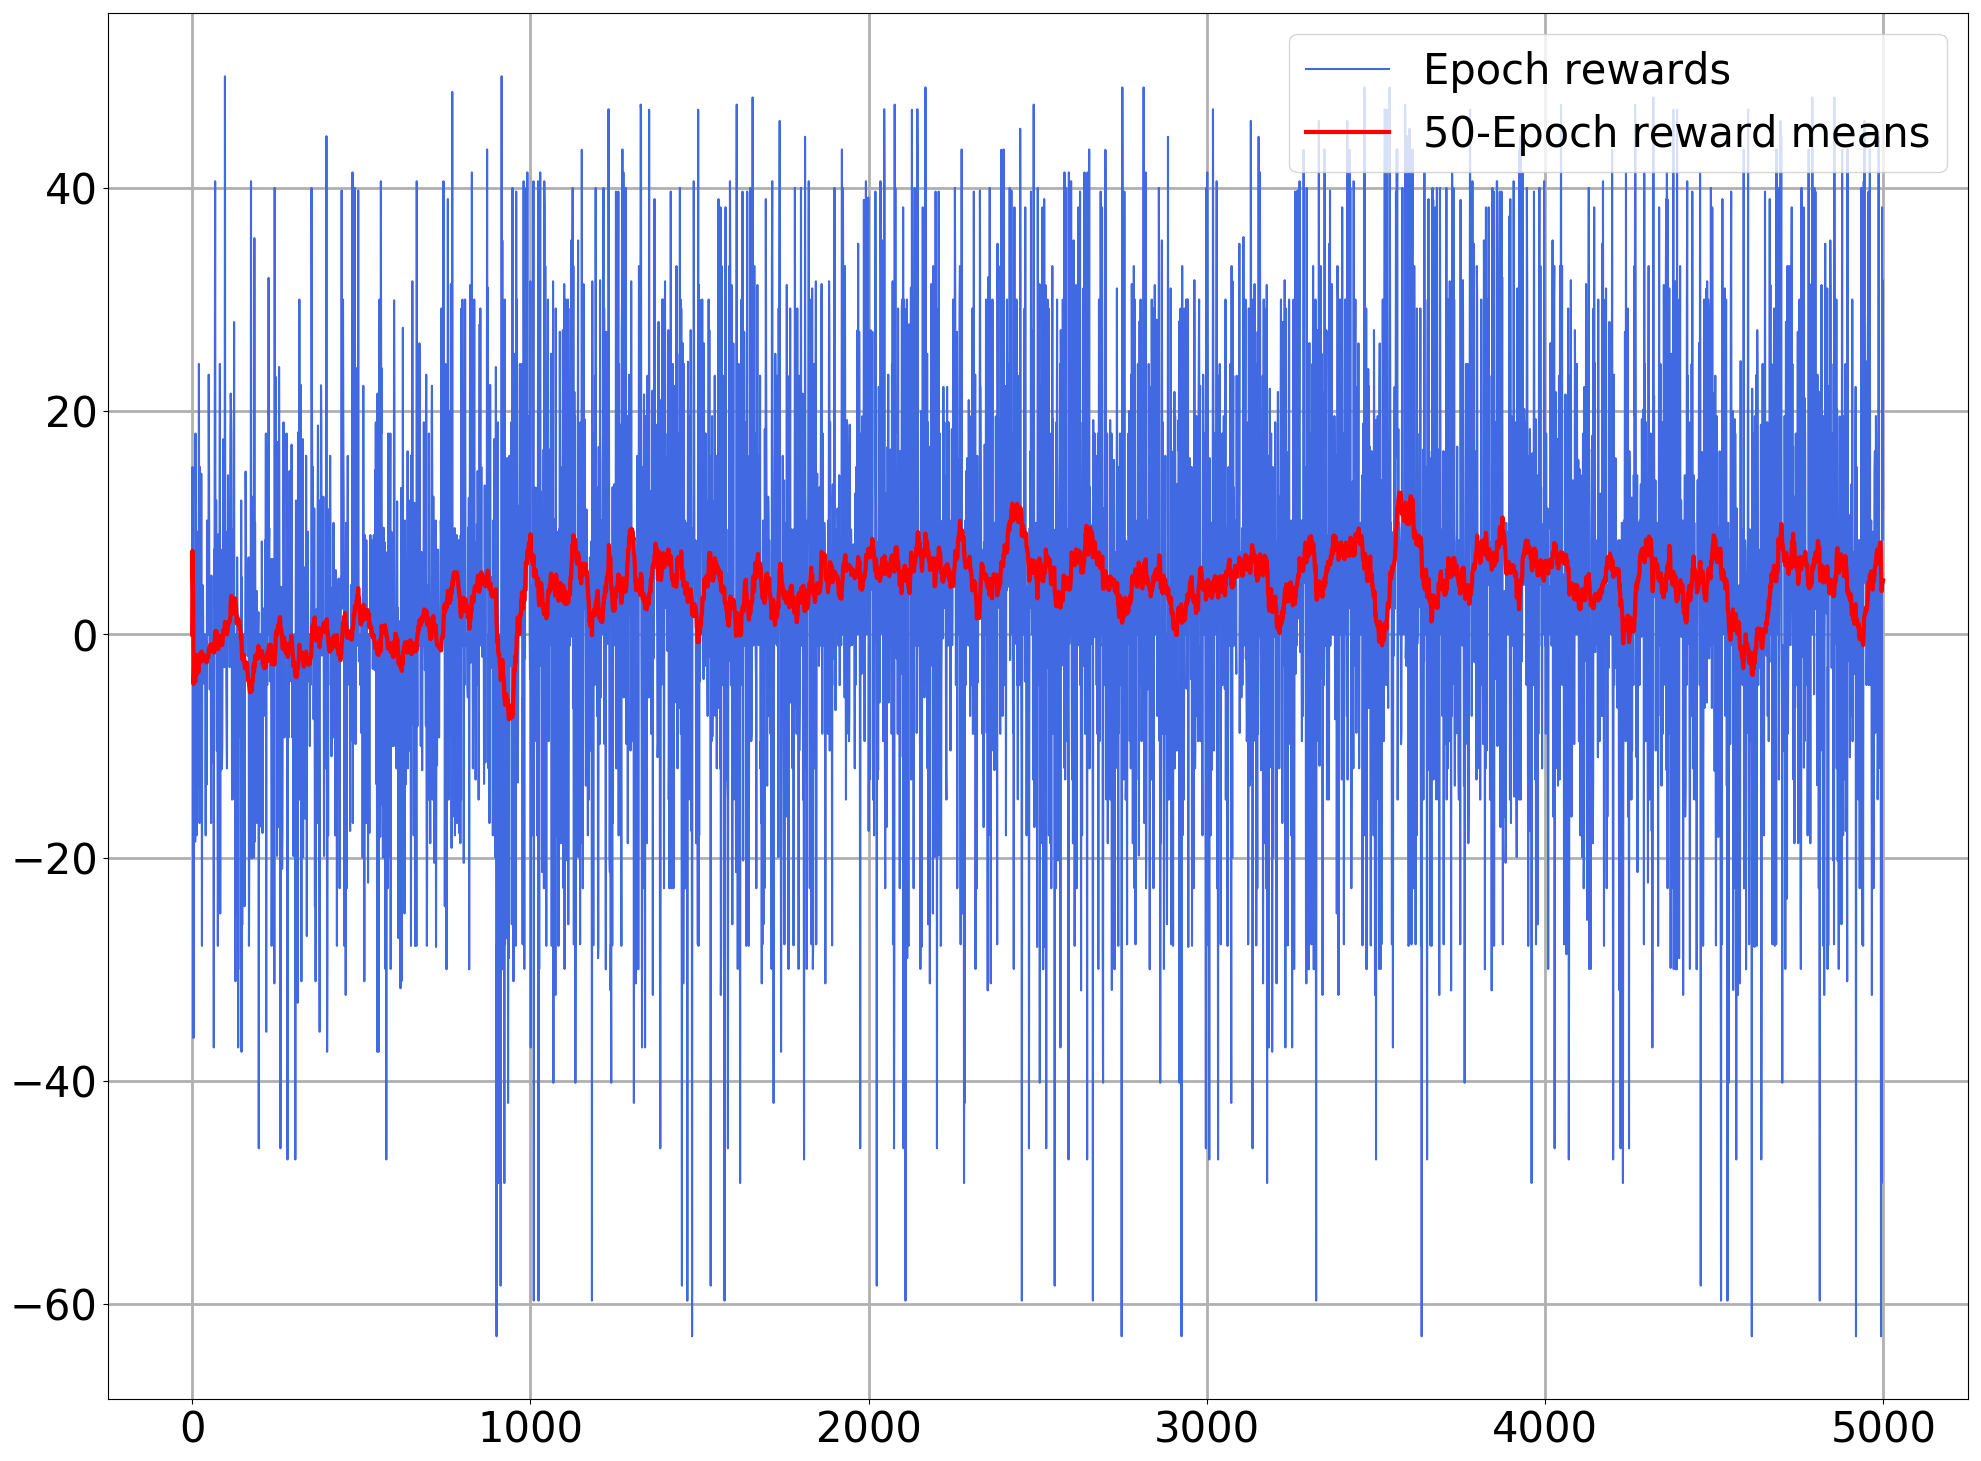
\includegraphics[width=\textwidth]{cnn_2_sell_trades_rewards.png}
        \caption{Mean rewards per epoch (sell)}
        \label{fig:analysis-dqn-1-trades-reward-sell}
    \end{subfigure}
    \begin{subfigure}[b]{0.45\textwidth}
        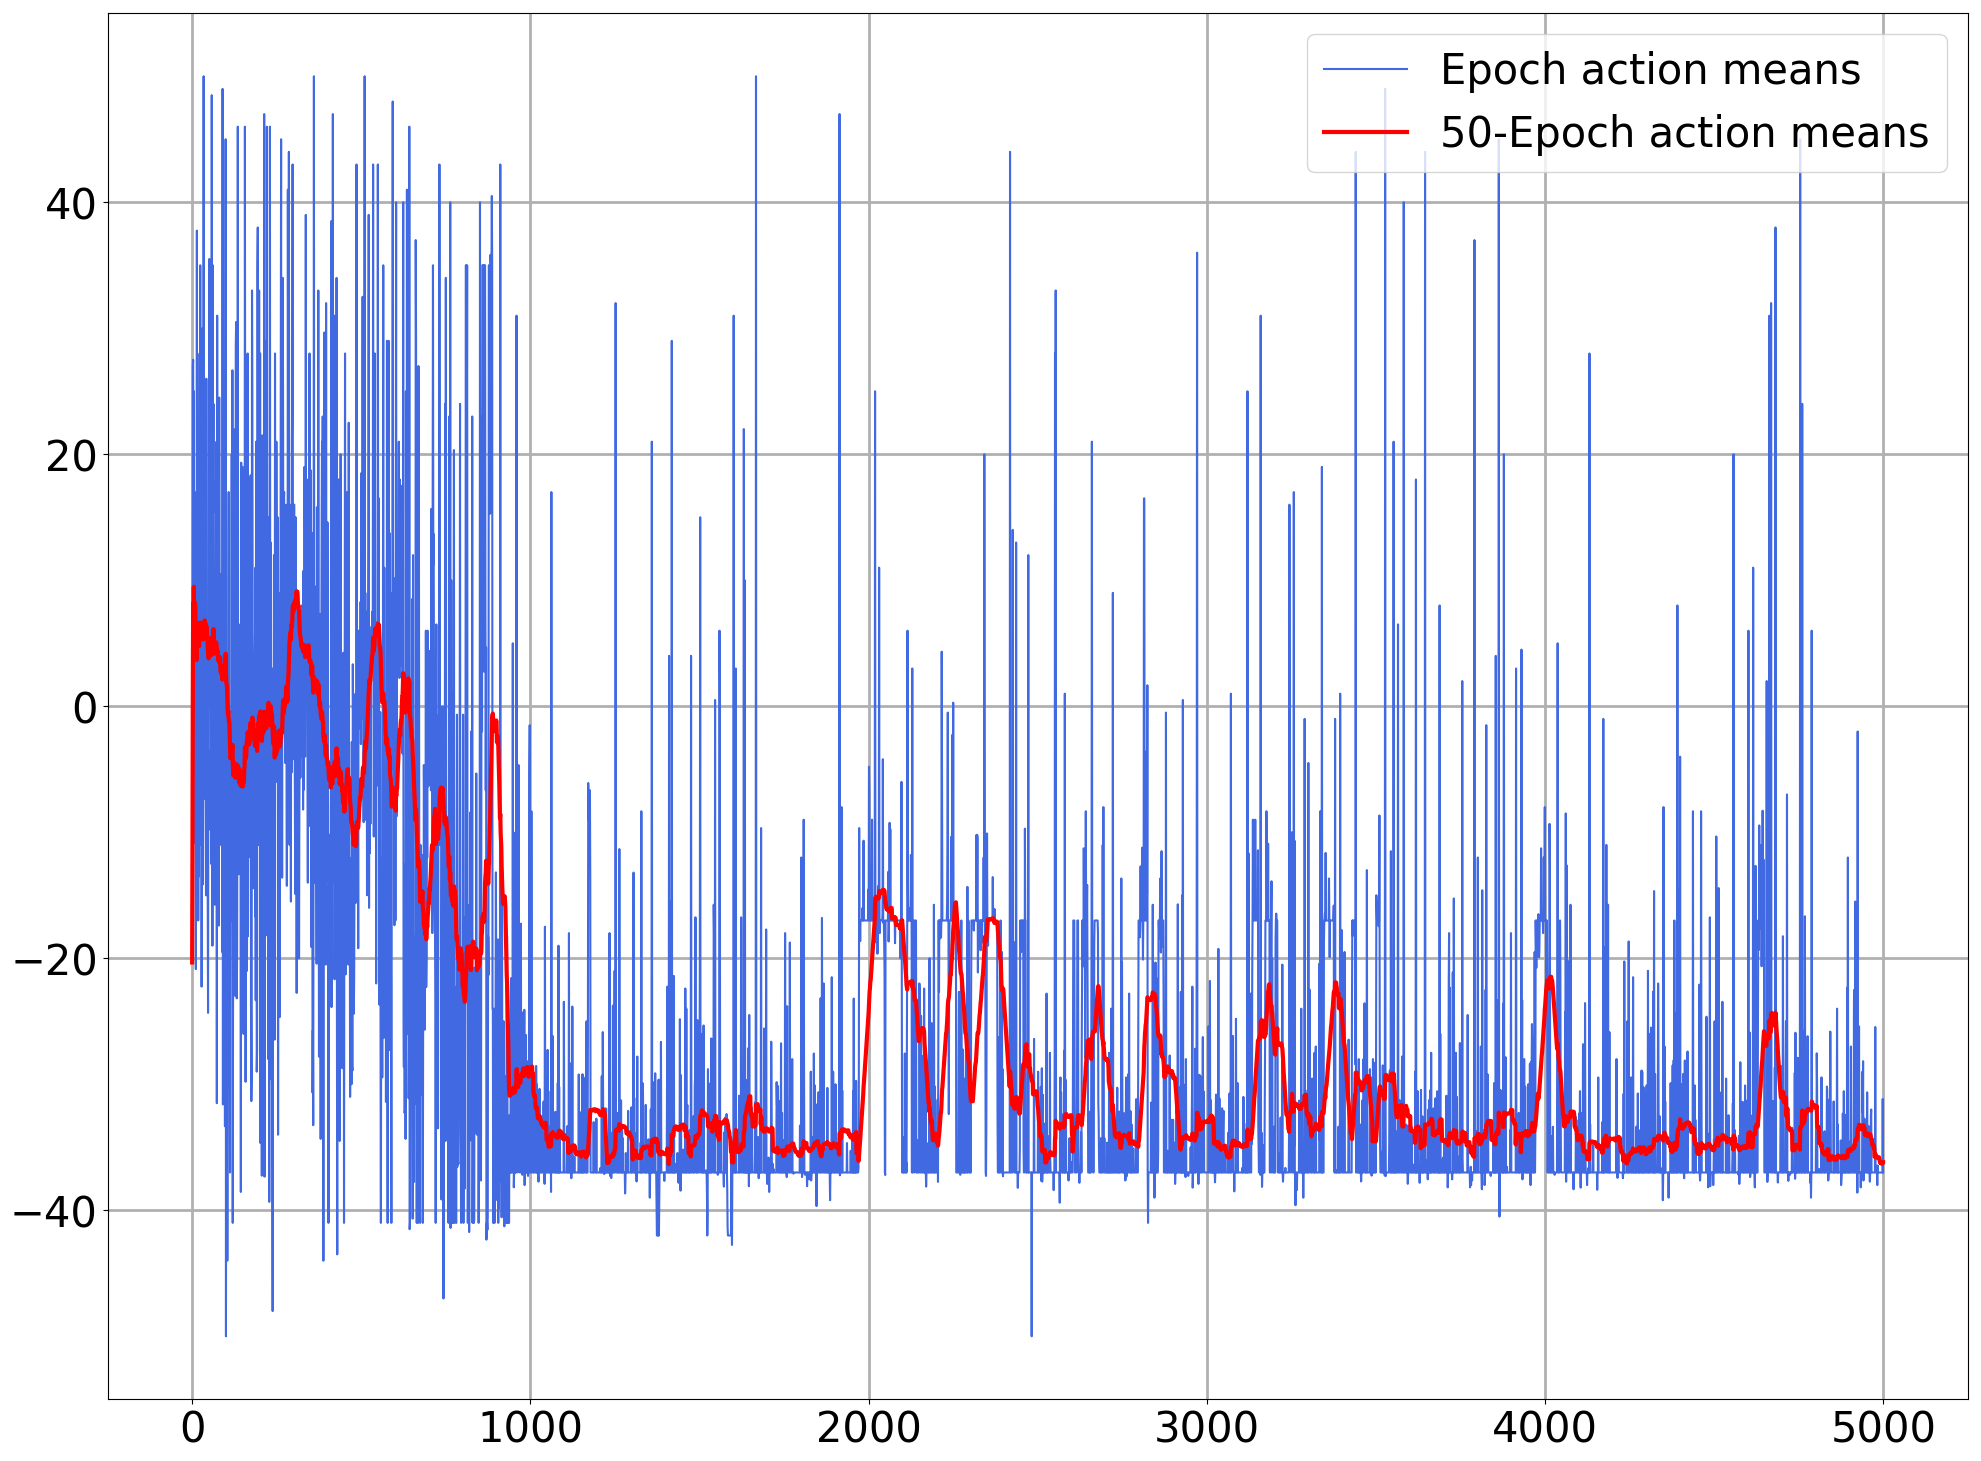
\includegraphics[width=\textwidth]{cnn_2_sell_trades_mean_actions.png}
        \caption{Mean of actions per epoch (sell)}
        \label{fig:analysis-dqn-1-trades-action-sell}
    \end{subfigure}
    \caption{DQN agent rewards and mean of actions for buying and selling on training data set II using feature II.}
    \label{fig:analysis-dqn-2}
\end{figure}

\section{Determining the limitations of the DQN agent}
\label{sec:eval-dqn-limitations}

\subsection{Conclusion of DQN approach}